\chapter{复数与三角函数}

\section{和角公式}

\begin{itemize}[leftmargin=\inteval{\myitemleftmargin}pt,itemsep=
   \inteval{\myitemitempsep}pt,topsep=\inteval{\myitemtopsep}pt]
\item 正余弦和角公式的图形证明。\\
\textbf{方法一}\ 在矩形$ ABCD $中,设$ AE=1,\angle AFE=\dfrac{\pi}{2},
\angle DAF=\alpha,\angle FAE=\beta $,则
\begin{align*}
AD=&\ BC=\cos\beta\cos\alpha=BE+EC=\cos(\alpha+\beta)+\sin\beta\sin\alpha  \\
AB=&\ DC=\sin(\alpha+\beta)=DF+FC=\cos\beta\sin\alpha+\sin\beta\cos\alpha  
\end{align*}
\begin{figure}[h]
\centering
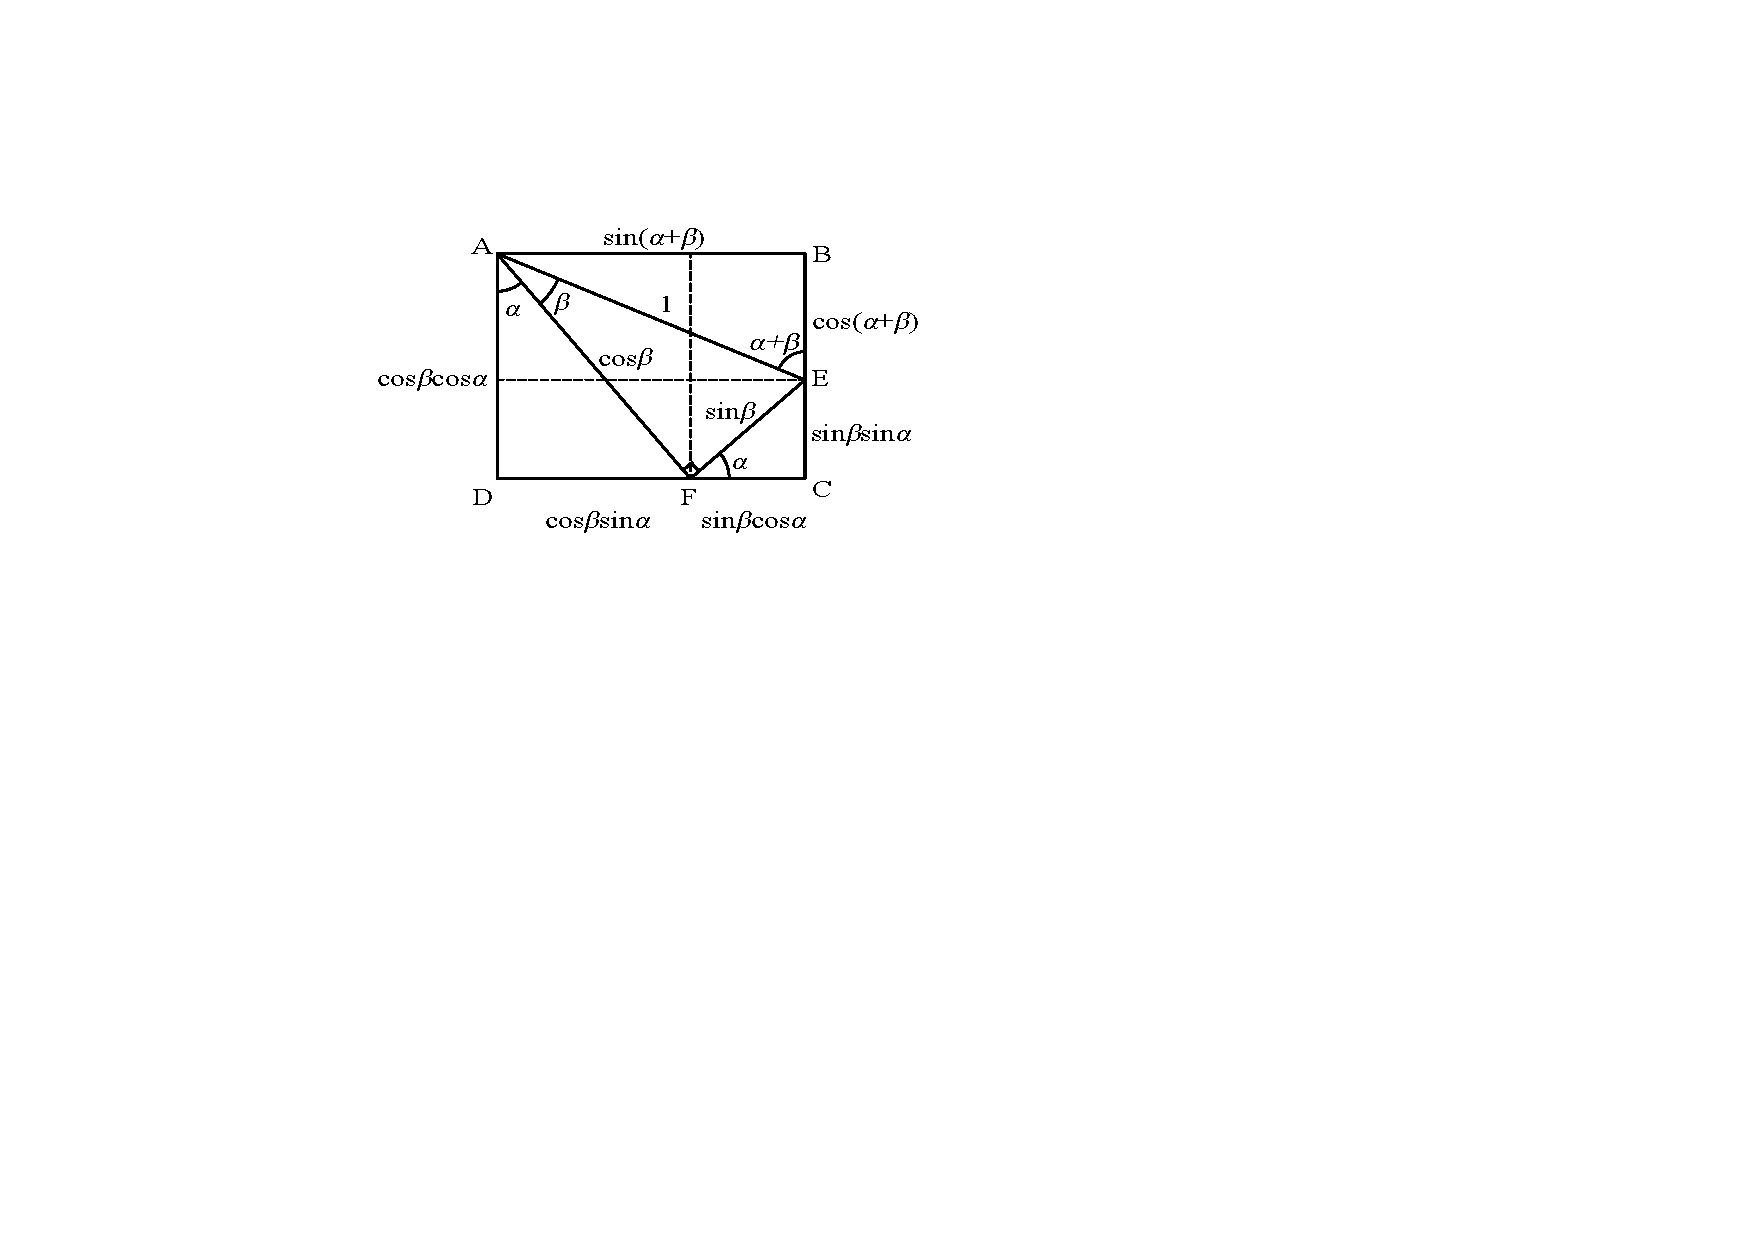
\includegraphics[width=0.4\linewidth]{正余弦和角公式图}
\end{figure}

\noindent \textbf{方法二}\ 利用三角形的外角等于不相邻两内角和的性质,
在$RT \Delta ABC $中,$ \angle C$是直角,延长$ CA $至$ D $点,
连接$ D,B $两点,设$ \angle ABD =\alpha $,$ \angle ADB =\beta $,
则$ \angle CAB =\alpha+\beta $. 
过$ A $点向$ BD $做垂线,垂足为$ E $点,在$ RT \Delta BCD $中使用勾股定理:
\begin{figure}[h]
\centering
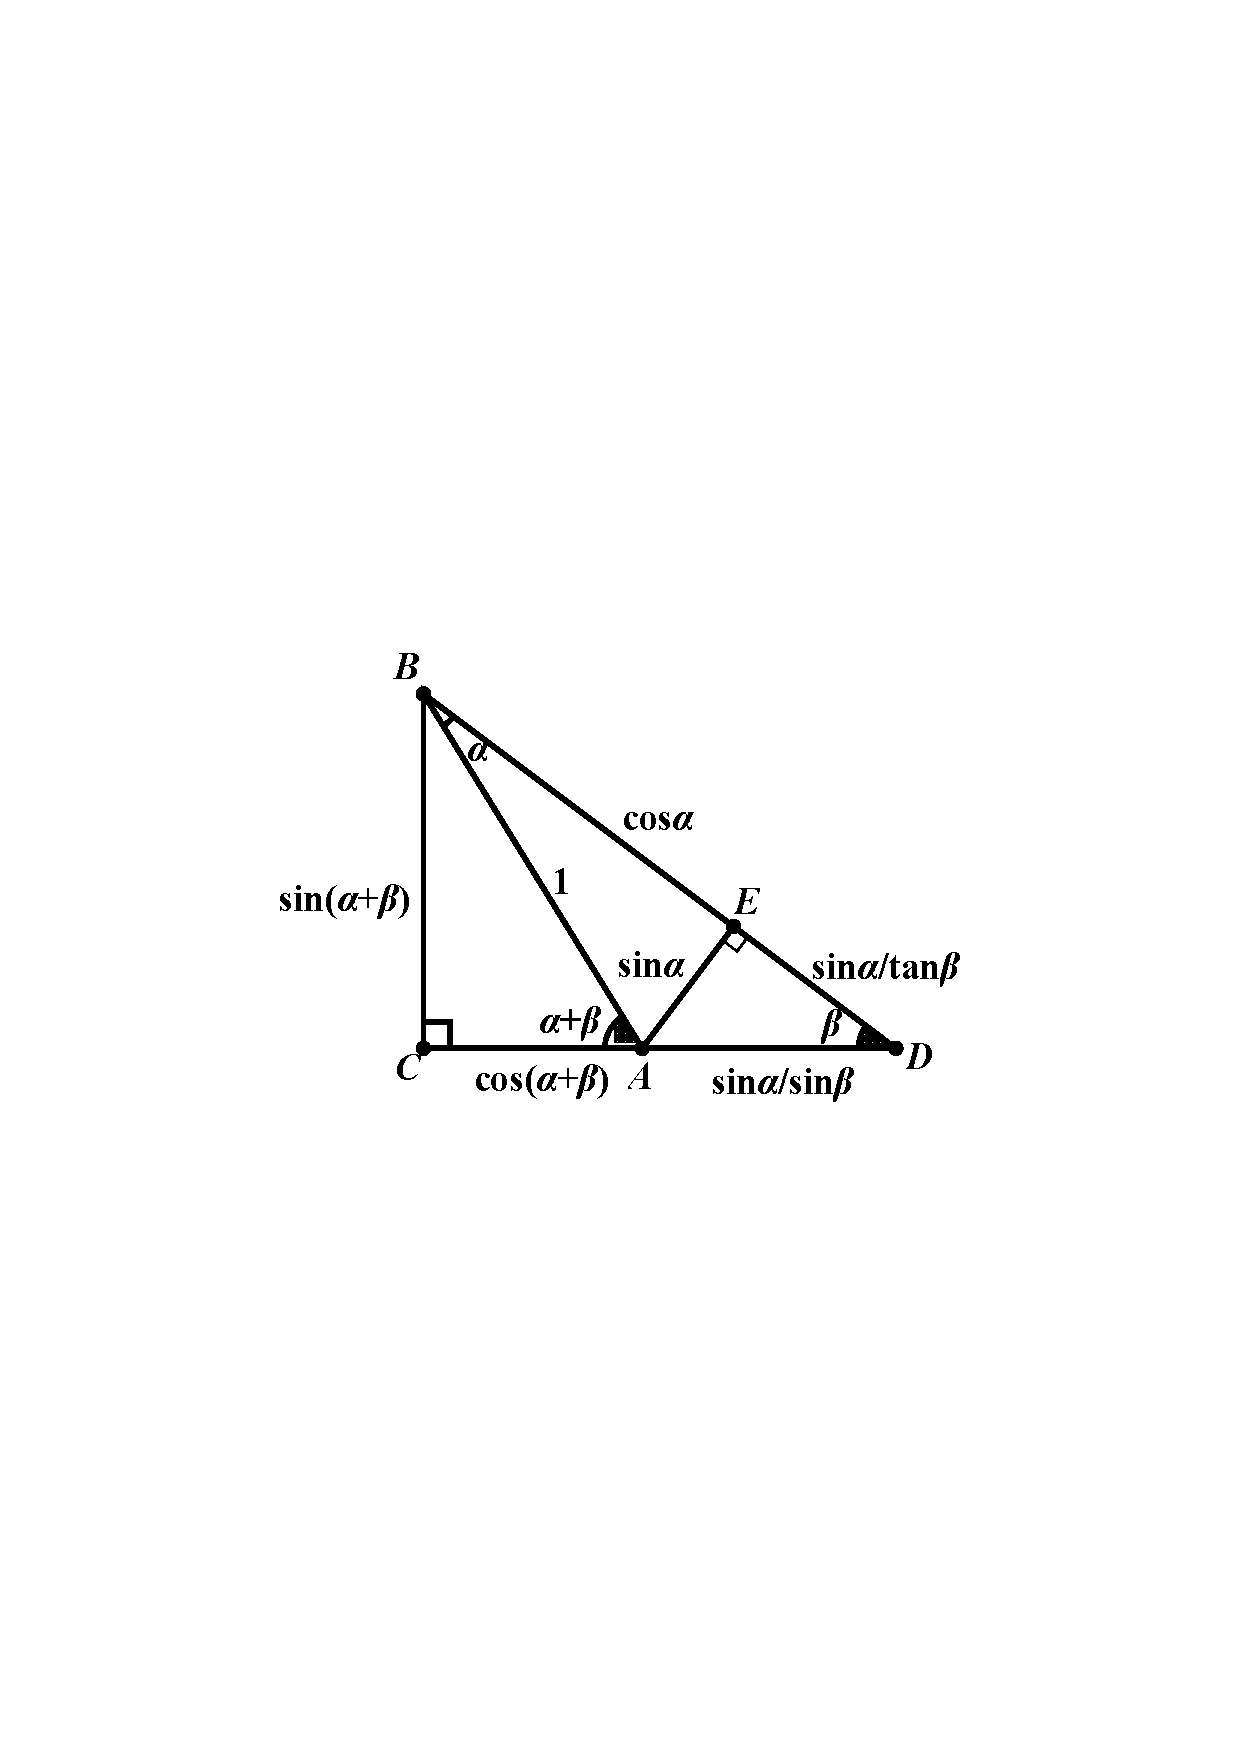
\includegraphics[width=0.3\linewidth]{余弦和角公式作图证明}
%    \caption{}
%    \label{fig:}
\end{figure}
% ~\newpage
\begin{align*}
\sin^2(\alpha +\beta )+\left[ \cos(\alpha +\beta )+\dfrac{\sin\alpha}{\sin\beta} \right] ^2 
=&\ \left( \cos\alpha +\dfrac{\sin\alpha}{\tan\beta }\right) ^2 \\
1+2\cos(\alpha +\beta )\dfrac{\sin\alpha}{\sin\beta}+\dfrac{\sin^2\alpha}{\sin^2\beta}=&\ 
\cos^2\alpha+2\dfrac{\sin\alpha \cos\alpha }{\tan\beta }+\dfrac{\sin^2\alpha}{\tan^2\beta }
\end{align*}
两边同乘$ \sin^2\beta $,移项,左侧只保留$ 2\cos(\alpha +\beta)\sin \alpha \sin\beta $,
然后约去$ 2\sin \alpha \sin\beta $,可得:
\begin{align*}
\cos(\alpha +\beta )=\cos \alpha \cos\beta - \sin \alpha \sin\beta 
\end{align*}

\item  正切半角公式的图形化证明。
\begin{figure}[H]
    \centering
    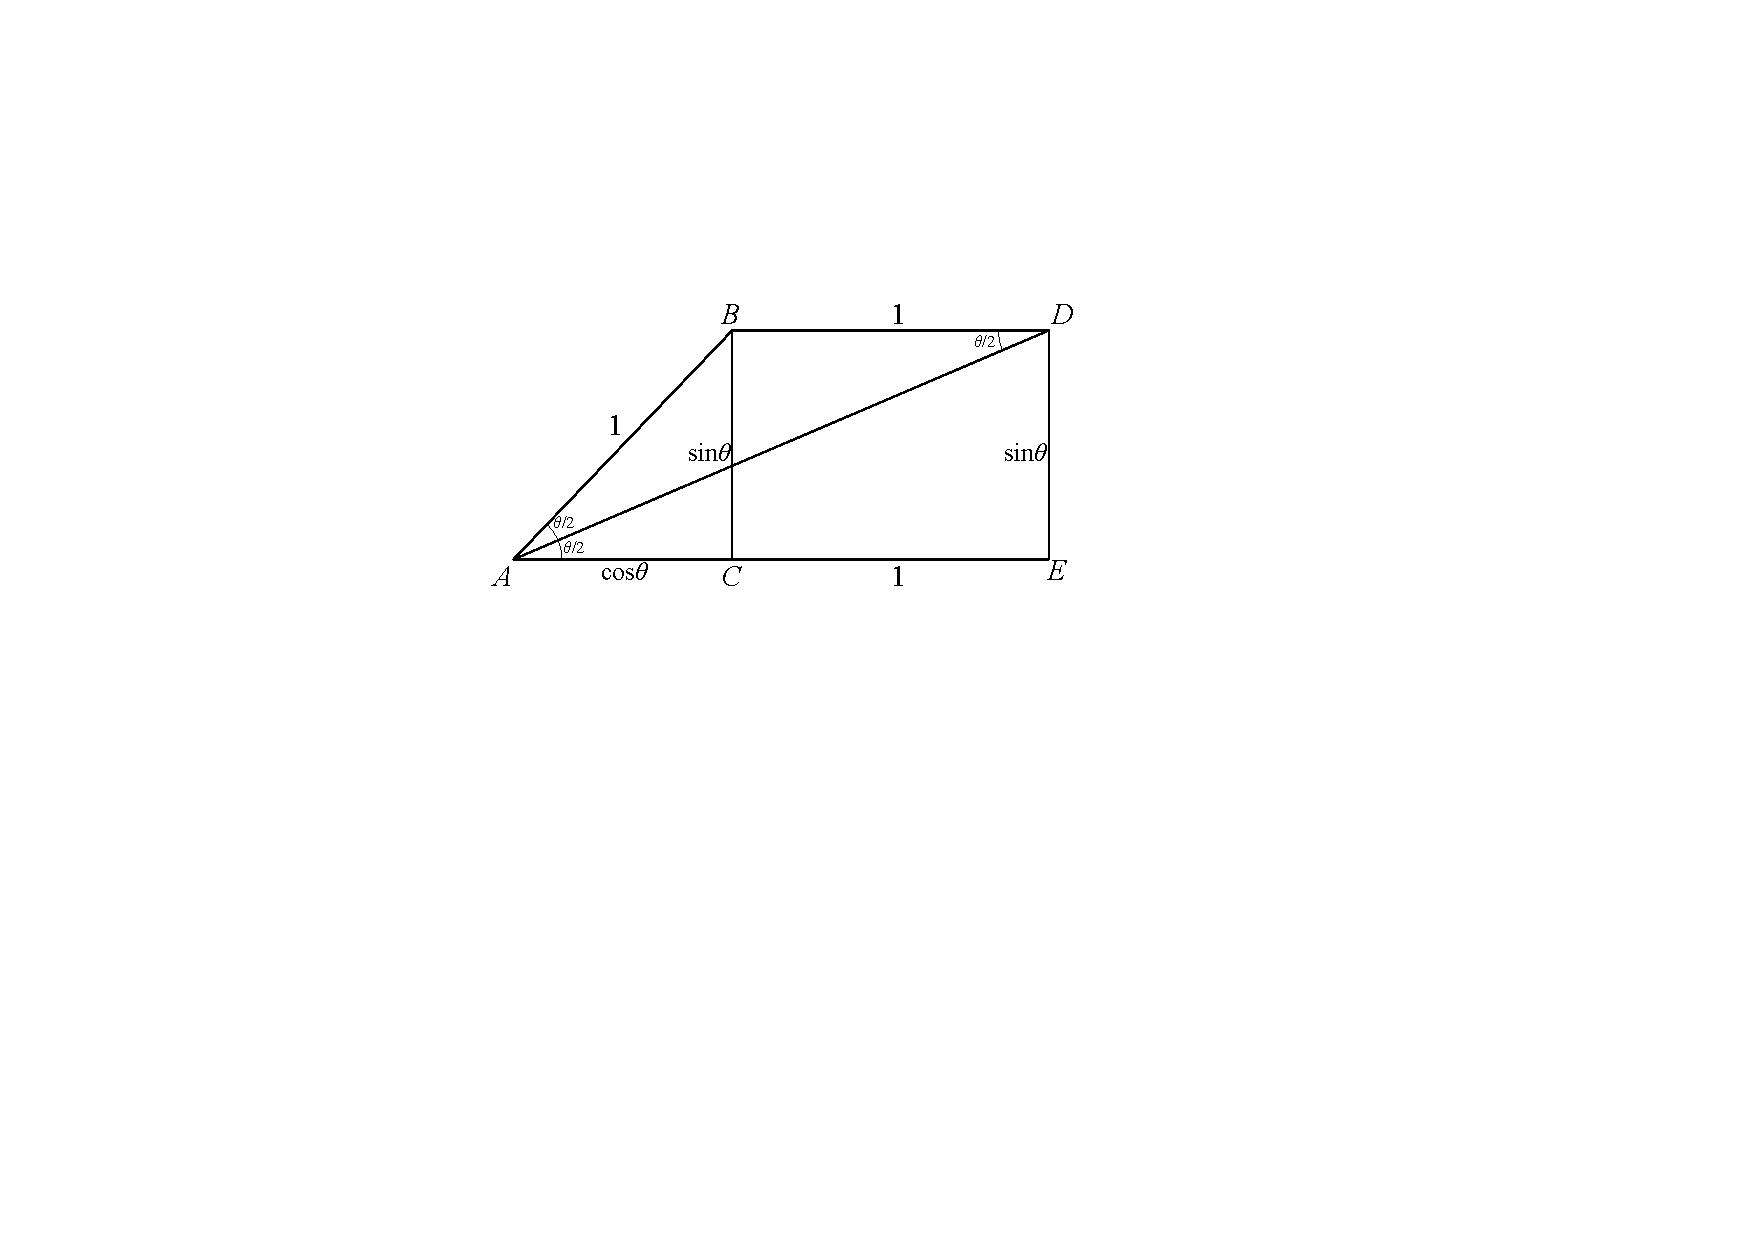
\includegraphics[width=0.5\linewidth]{PDF_Picture/正切半角公式的图形化证明}
\end{figure}
设$|BA|=|BD|=|CE|=1$,$\angle BAC=\theta$,
$\angle BCA $为直角,则
\begin{gather*}
    \tan\dfrac{\theta}{2}=\dfrac{|DE|}{|AE|}=
    \dfrac{|DE|}{|AC|+|CE|}=\dfrac{\sin\theta}{\cos\theta+1}
\end{gather*}

\item 两个角正弦、余弦、正切的和角、差角公式:
\begin{align*} 
\sin(\alpha\pm\beta)=&\ \sin\alpha\cos\beta \pm
 \cos\alpha\sin\beta \\
\cos(\alpha\pm\beta)=&\ \cos\alpha\cos\beta \mp
 \sin\alpha\sin\beta \\
\tan(\alpha\pm\beta)=&\ \dfrac{\tan \alpha\pm\tan \beta}
 {1\mp \tan \alpha \tan \beta} 
\end{align*}

\item 和差化积:
\begin{align*}
\sin x+\sin y=&\  \sin \left(\dfrac{x+y}{2} +\dfrac{x-y}{2} \right) +\sin \left(\dfrac{x+y}{2}-\dfrac{x-y}{2} \right)\\
=&\  2\sin \left(\dfrac{x+y}{2}\right) \cos\left(\dfrac{x-y}{2}\right) \\ 
\cos x+\cos y=&\  \cos \left(\dfrac{x+y}{2} +\dfrac{x-y}{2} \right) +\cos \left(\dfrac{x+y}{2}-\dfrac{x-y}{2} \right)\\
=&\  2\cos \left(\dfrac{x+y}{2}\right) \cos  \left(\dfrac{x-y}{2}\right)	
\end{align*}
\item 积化和差:
\begin{align*}
\sin x\sin y=&\ \dfrac{1}{2}[\cos(x-y)-\cos(x+y)] \\
\cos x\cos y=&\ \dfrac{1}{2}[\cos(x-y)+\cos(x+y)] \\	
\sin x\cos y=&\ \dfrac{1}{2}[\sin(x+y)+\sin(x-y)] 
\end{align*}
\begin{align*}
\sin(x-y)\sin(x+y) =&\ \sin^2 x-\sin^2y=\cos^2 y-\cos^2 x \\
=&\ (\sin x-\sin y)(\sin x+\sin y)=(\cos y-\cos x)(\cos y+\cos x) \\
\cos(x-y)\cos(x+y) =&\ \cos^2 x+\cos^2 y-1=1-\sin^2 x-\sin^2 y \\
=&\ \cos^2 x-\sin^2 y=\cos^2 y-\sin^2 x \\
=&\ (\cos x-\sin y)(\cos x+\sin y)=(\cos y-\sin x)(\cos y+\sin x)
\end{align*}

\item 辅助角公式:
\begin{align*}
a\sin x+b\cos x 
=&\  \sqrt{a^2+b^2}\left(\dfrac{a}{\sqrt{a^2+b^2}}\sin x+\dfrac{b}{\sqrt{a^2+b^2}}\cos x \right) \\
=&\  \sqrt{a^2+b^2}\left(\cos\varphi\sin x+\sin\varphi\cos x \right) \\
=&\  \sqrt{a^2+b^2}\sin(x+\varphi) \quad\quad 
\left(\tan \varphi=\dfrac{b}{a}\right)
\end{align*}
变体一:
\begin{align*}
a\sin x+b\cos (x+x_0) 
=&\  a\sin x+b\cos x\cos x_0-b\sin x\sin x_0 \\
=&\  (a-b\sin x_0)\sin x+(b\cos x_0)\cos x \\
=&\  \sqrt{a^2+b^2-2ab\sin x_0}\sin(x+\varphi) 
\end{align*}
变体二:
\begin{align*}
&a\cos^2x+b\sin^2x+c\sin x\cos x \\
=&\  a\dfrac{\cos2x+1}{2} +b\dfrac{-\cos2x+1}{2}+\dfrac{c}{2}\sin2x \\
=&\  \dfrac{a-b}{2}\cos2x+\dfrac{c}{2}\sin2x+\dfrac{a+b}{2} \\
=&\  \dfrac{1}{2}\sqrt{(a-b)^2+c^2}\sin(2x+\varphi)+\dfrac{a+b}{2}
\end{align*}
变体三:
\begin{align*}
a\sin^2x+b\cos x=a(1-\cos^2x)+b\cos x=
-a\left( \cos x-\dfrac{b}{2a}\right) ^2+\dfrac{b^2}{4a}
\end{align*}

\item $ ^* $ 三个角之和的正、余弦公式
\footnote{这几个公式在笔者的工作中经常遇到,在多轴机械臂的运动控制中,
    如果5轴或6轴的机械臂存在连续3根轴是平行的,那么其正向运动学计算就需要
    用到三个角的和与差的正余弦公式,而逆向运动学存在解析解。
    5轴码垛机械臂就是典型的存在连续3根平行轴的机械臂,其2、3、4号轴是平行的,
    且都与1、5号轴垂直。挖掘机也存在连续3根平行轴。}:
\begin{align*}
    &\sin(\alpha+\beta+\gamma)\\
    =&-\sin\alpha\sin\beta\sin\gamma
    +\sin \alpha \cos \beta \cos \gamma  + \cos \alpha \sin \beta 
    \cos \gamma + \cos \alpha \cos \beta \sin \gamma  \\
    &\cos(\alpha+\beta+\gamma)\\ 
    =& \cos \alpha \cos \beta \cos\gamma
    -\cos\alpha  \sin \beta \sin \gamma - \sin \alpha \sin \beta 
    \cos \gamma - \sin \alpha \cos \beta \sin \gamma
\end{align*}
$ \sin(\alpha+\beta+\gamma) $展开式的特点是会含有三个$ \sin $
的乘积的项,其余三项都是两个$ \cos $,一个$ \sin $,
$ \sin $的总数等于$ \cos $的总数(都是6个)。
$ \cos(\alpha+\beta+\gamma) $展开式有类似性质,会含有三个
$ \cos $的乘积的项,其余三项都是两个$ \sin $,一个$ \cos $,
$ \sin $的总数等于$ \cos $的总数(都是6个)。

因为两个角的正、余弦的和(差)角公式,$ \sin $的数量等于$ \cos $
的数量,多个角的和与差展开,就是反复运用两个角的和与差展开,
所以$ \sin $的数量会始终等于等于$ \cos $的数量。
手工计算时可以利用这一性质进行快速检查,若发现数量不相等,
则肯定存在错误。

\item $^*$ 双曲正弦函数 $ \sinh x=\dfrac{\e^x-\e^{-x}}{2} $, 双曲余弦函数
$\cosh x=\dfrac{\e^x+\e^{-x}}{2} $,这两个函数存在与$ \sin x,\cos x $
类似的和角、差角、二倍角、积化和差、和差化积公式。
\begin{align*}
& (\sinh x)'=\cosh x\\
& (\cosh x)'=\sinh x \\
& \cosh^2 x-\sinh^2 x=1 \\
& \sinh(x\pm y)=\sinh x\cosh y\pm \cosh x\sinh y \\
& \cosh(x\pm y)=\cosh x\cosh y\pm \sinh x\sinh y \\
& \sinh(2x)=2\sinh x\cosh x \\
& \cosh(2x)=\cosh^2 x+\sinh^2 x \\
& \sinh x\pm \sinh y=2\sinh\left(\dfrac{x\pm y}{2}\right)
\cosh\left(\dfrac{x\mp y}{2}\right) \\
& \cosh x+\cosh y   =2\cosh\left(\dfrac{x+y}{2}\right)
\cosh\left(\dfrac{x-y}{2}\right) 
\end{align*}

双曲正弦$ y=\sinh x $的反函数为$ y=\ln(x+\sqrt{x^2+1})\ (x\in\textbf{R}) $;\\
双曲余弦$ y=\cosh x\ (x\geq 0) $的反函数为$ y=\ln(x+\sqrt{x^2-1})\ (x\geq 1) $.

\end{itemize}

\section{三次方程求根公式}
\begin{itemize}[leftmargin=\inteval{\myitemleftmargin}pt,itemsep=
   \inteval{\myitemitempsep}pt,topsep=\inteval{\myitemtopsep}pt]
\item 奇数次多项式至少存在一个实零点,实零点的数量也一定是奇数。
偶数次多项式可能没有实零点,实零点的数量一定是偶数(包括0个),
一定存在极大值或极小值。

\item 对于任意三次方程$ ax^3+bx^2+cx+d=0 $,可先除以非零的$ a $,把三次项系数化为1,
再通过平移变换$ x=t-\dfrac{b}{3a} $,消去三次方程的二次项,故只需考虑形如$ x^3+px+q=0 $的三次方程。
引入新的未知数$ u,v $,并假设$ x=u+v $,则
\begin{gather*}
    x^3=u^3+v^3+3uv(u+v)=u^3+v^3+3uvx  \\
     x^3-3uvx-(u^3+v^3)=0
\end{gather*}
比较系数可得:
$ \begin{cases}
-3uv = p \ \left(u^3v^3=-\dfrac{p^3}{27} \right) \\
-(u^3+v^3) = q
\end{cases} \vspace{-4mm} $,于是,$ u^3,v^3 $是二次方程$ y^2+qy-\dfrac{p^3}{27}=0 $的根,二次方程的判别式除以4以后仍用
$ \Delta $表示,$ \Delta=\dfrac{q^2}{4}+\dfrac{p^3}{27} $. 解二次方程可得:
$ u^3=-\dfrac{q}{2} + \sqrt{\Delta},\ v^3=-\dfrac{q}{2} - \sqrt{\Delta}$.
再令$ \omega=-\dfrac{1}{2}+\dfrac{\sqrt{3}}{2}\i =
\cos(\dfrac{2\pi}{3})+\i\sin(\dfrac{2\pi}{3})=\e^{\i\frac{2\pi}{3}}$,则$ \omega^3=1 $, 那么三次方程$ x^3+px+q=0 $的求根公式可表达如下:
\begin{align*}
\begin{cases}
    x_1= \sqrt[3]{-\dfrac{q}{2} + \sqrt{\Delta}}+
    \sqrt[3]{-\dfrac{q}{2} - \sqrt{\Delta}} \\
    x_2= \omega\sqrt[3]{-\dfrac{q}{2} + \sqrt{\Delta}}+
    \omega^2\sqrt[3]{-\dfrac{q}{2} - \sqrt{\Delta}} \\
    x_3= \omega^2\sqrt[3]{-\dfrac{q}{2} + \sqrt{\Delta}}+
    \omega\sqrt[3]{-\dfrac{q}{2} - \sqrt{\Delta}} 
\end{cases} 
\end{align*}
大家可能觉得$ \Delta=\dfrac{q^2}{4}+\dfrac{p^3}{27} $难以记忆,
其实,只要使用量纲分析,就不算困难。对于三次方程$ x^3+px+q=0 $,
如果认为$ x $代表长度,那么$ p $就是面积(长度的2次方),
$ q $就是体积(长度的3次方),
$ p^3 $和$ q^2 $具有相同的单位(都是长度的6次方),
否则两者不能进行加法运算,再把$ \Delta $写成
$ \Delta=\dfrac{q^2}{2^2}+\dfrac{p^3}{3^3} $就好记了。

\item 对于一般的四次函数$ ax^4+bx^3+cx^2+dx+e $,
做平移$ x=t-\dfrac{b}{4a} $,可以消去三次项。
四次方程也有求根公式,而五次及更高次的一般方程,没有求根公式。

\item 形如$ ax^4+bx^3+cx^2\pm bx+a=0 $的特殊四次方程,可以通过将方程
整体除以$ x^2 $,再作换元$ u=x\pm \dfrac{1}{x} $进行求解。
比如$ bx $前面取“+”时,
\begin{gather*}
    ax^4+bx^3+cx^2+bx+a=0 \\
    ax^2+bx+c+\dfrac{b}{x}+\dfrac{a}{x^2}=0 \\
    a\left(x^2+\dfrac{1}{x^2}\right)+b\left(x+\dfrac{1}{x}\right)+c=0 \\
    a\left[\left(x+\dfrac{1}{x}\right)^2-2\right]+b
    \left(x+\dfrac{1}{x}\right)+c=0 \\
    au^2+bu+(c-2a)=0
\end{gather*}

\item 三次函数$ y =ax^3+cx+d $上的点$ (x_0,y_0) $
处的切线斜率计算:
\begin{align*}
\begin{cases}
    y =&\ k(x-x_0)+y_0  \\
    y =&\ ax^3+cx+d
\end{cases}
\end{align*}
其中,$ y_0=ax_0^3+cx_0+d $,消去$ y $可得:
\begin{gather*}
ax^3+(c-k)x+(kx_0-ax_0^3-cx_0)=0 \\
\Delta=\dfrac{(c-k)^3}{27a^3}+\dfrac{(kx_0-ax_0^3-cx_0)^2}{4a^2}=0 \\
k=3ax_0^2+c
\end{gather*}

\end{itemize}

\section{复数的一些性质}
\begin{itemize}[leftmargin=\inteval{\myitemleftmargin}pt,itemsep=
   \inteval{\myitemitempsep}pt,topsep=\inteval{\myitemtopsep}pt]
\item 虚数单位$ \i $的整数次幂的周期性:
$ \i^{4n}=1,\ \i^{4n+1}=\i,\ \i^{4n+2}=-1,\ \i^{4n+3}=-\i $.  

\item 共轭复数的性质:$ \overline{\overline{z}}=z,\ 
\overline{z_1\pm z_2}=\overline{z_1}\pm \overline{z_2},\ 
\overline{z_1\cdot z_2}=\overline{z_1}\cdot \overline{z_2},\ 
\overline{\dfrac{z_1}{z_2}}=\dfrac{\overline{z_1}}
{\overline{z_2}} $.  

\item 复数的模的性质:$ |z|=|\overline{z}|,\ z\overline{z}=
|z|^2=|\overline{z}|^2,\ |z_1z_2|=|z_1||z_2|,\ \left|\dfrac{z_1}{z_2}\right|=
\dfrac{|z_1|}{|z_2|} $. \\
对于向量$ \vec{a} $,有$ \vec{a}^2=
|\vec{a}|^2 $,而对于不是实数的复数$ z=a+b\i $,有
$ z^2=a^2-b^2+2ab\i \neq |z|^2=a^2+b^2 $. 

\item $ \left||z_1|-|z_2|\right|\leq |z_1\pm z_2|
\leq|z_1|+|z_2| $. \quad
$ |z_1+z_2|^2+|z_1-z_2|^2=2\left( |z_1|^2+|z_2|^2 \right) $. 

\item 没有实根的偶数次多项式,总能写成两个更低次数的多项式的平方和,
而且写法不唯一。比如:
\begin{align*}
 &\ x^4+2x^3+11x^2+18x+18 \\
=&\  (x^2+2x+2)(x^2+9)  \\
=&\  [(x+1-\i)(x+1+\i)][(x-3\i)(x+3\i)] \\
=&\  [(x+1-\i)(x-3\i)][(x+1+\i)(x+3\i)] \\
=&\  [(x^2+x-3)-(4x+3)\i][(x^2+x-3)+(4x+3)\i] \\
=&\  (x^2+x-3)^2+(4x+3)^2  \\
=&\  [(x+1-\i)(x+3\i)][(x+1+\i)(x-3\i)] \\
=&\  (x^2+x+3)^2+(2x+3)^2
\end{align*}

\item 考虑$ x^n+1 $,如果$ n $含有一个大于2的质因子,比如$ n=ps $,其中$ p $
是大于2的质因子(当然也是一个奇数),
那么
\begin{gather*}
    x^n+1=1-(-x^s)^p=[1-(-x^s)][1+(-x^s)+(-x^s)^2-\cdots +(-x^s)^{p-1}]
\end{gather*}
如果$ n=2^r $,那么$ x^n+1 $在实数范围内无法分解出一次的因式。比如
\begin{align*}
x^4+1 =&\  (x^2-\sqrt{2}x+1)(x^2+\sqrt{2}x+1)   \\
=&\  \left[x-\left(\dfrac{\sqrt{2}}{2}+\dfrac{\sqrt{2}}{2}\i \right)\right] 
\left[x-\left( \dfrac{\sqrt{2}}{2}-\dfrac{\sqrt{2}}{2}\i \right)\right]
\cdot \\
&\ \left[x-\left(-\dfrac{\sqrt{2}}{2}+\dfrac{\sqrt{2}}{2}\i \right)\right]
\left[x-\left(-\dfrac{\sqrt{2}}{2}-\dfrac{\sqrt{2}}{2}\i \right)\right]  \\
x^8+1 =&\  \left( x^2+\sqrt{2+\sqrt{2}}\ x+1\right) \cdot
\left( x^2-\sqrt{2+\sqrt{2}}\ x+1\right) \cdot \\
&\ \left( x^2+\sqrt{2-\sqrt{2}}\ x+1\right) \cdot
\left( x^2-\sqrt{2-\sqrt{2}}\ x+1\right)
\end{align*}

\item 考虑$ x^{n}+a^n=0\ (a>0) $,它的$ n $个复数根为
$ x=a\e^{\i\frac{1+2k}{n}\pi} ,\ k=0,1,2\cdots ,(n-1) $. 
取其中两个互为共轭的根,作如下乘法:
\begin{gather*}
    \left(x-a\e^{\i\frac{1+2k}{n}\pi}\right)
    \left(x-a\e^{-\i\frac{1+2k}{n}\pi}\right)=
    x^2-2ax\cos\left(\dfrac{1+2k}{n}\pi\right) +a^2    
\end{gather*}
上式右侧便是$ x^n+a^n $的一个二次因式。比如$ n=5 $时,
\begin{align*}
    x^5+a^5 &=(x+a)\left(x^2-2ax\cos\dfrac{\pi}{5}+a^2 \right)
    \left(x^2-2ax\cos\dfrac{3\pi}{5}+a^2 \right) \\
    &=(x+a)\left(x^2-\dfrac{\sqrt{5}-1}{2} ax+a^2 \right)
    \left(x^2+\dfrac{\sqrt{5}-1}{2} ax+a^2 \right)
\end{align*}

%\item 考虑两个复数的除法,$ \dfrac{A+B\i}{C+D\i}=P+Q\i\ (CD\neq 0) $,那么
%\begin{align}\label{复数除法比较性能}
%    P=\dfrac{AC+BD}{C^2+D^2},\q Q=\dfrac{BC-AD}{C^2+D^2}  
%\end{align}
%现在要编一段计算机程序,在已知$ A, B, C, D $的情况下求$ P,Q $.
%如果直接按上面的计算公式编程,至少需要进行6次浮点数乘法运算
%2次浮点数除法运算,2次浮点数加法和1次浮点数减法。至少6次乘法是
%因为$ C^2+D^2 $算过以后可以用一个变量$ E $来保存,
%省掉了2次乘法和1次加法,即
%\begin{align*}
%    E &=C^2+D^2\\
%    P &=\dfrac{AC+BD}{E},\q Q=\dfrac{BC-AD}{E}
%\end{align*}
%将以上算法暂时命名为“直接算法”。请读者思考,是否有办法减少乘法的次数?
%在知名的开源线性代数库LAPACK中,有一个名叫dladiv.f的
%Fortran语言代码文件,里面提供的函数就是来计算$ P,Q $的,
%这种十分在意性能的数学库采取了什么方法来计算
%$ P,Q $呢?实际上就是对(\ref{复数除法比较性能})式进行了等价的变形,
%分子分母同时除以$ C $,得
%\begin{align*}
%    P=\frac{A+B\cdot\frac{D}{C}}{C+D\cdot\frac{D}{C}},\q
%    Q=\frac{B-A\cdot\frac{D}{C}}{C+D\cdot\frac{D}{C}}
%\end{align*}
%引入两个新的变量$ E=\dfrac{D}{C},\ F=C+DE $,那么
%\begin{gather*}
%    P=\dfrac{A+BE}{F},\q Q=\dfrac{B-AE}{F}
%\end{gather*}
%在这种算法中,共有3次乘法,3次除法,2次加法和1次减法。以增加1次除法
%为代价,减少了3次乘法。假如乘法和除法的耗时几乎一样,那么LAPACK
%中的算法效率更高。假如除法的耗时明显比乘法长,那么直接算法可以修改为
%\begin{align*}
%    E &=\dfrac{1}{C^2+D^2} \\
%    P &=(AC+BD)E,\q Q=(BC-AD)E
%\end{align*}
%总共8次乘法,1次除法,加减法次数不变。LAPCAK中的方法可以修改为
%\begin{align*}
%    E &=\dfrac{D}{C},\q F=\dfrac{1}{C+DE} \\
%    P &=(A+BE)F,\q Q=(B-AE)F
%\end{align*}
%总共5次乘法,2次除法,加减法次数不变。与“6乘2除”的直接算法相比肯定更快。
%但与“8乘1除”相比哪个更快,结论并不确定,与执行计算的硬件有关。
%感兴趣的读者可以用C++写程序,在Visual Studio中或者去网站
%https://quick-bench.com上对比一下上面4种写法的速度差异。


\end{itemize}

%\section{反三角函数}

%\end{itemize}

\section{欧拉公式$ \e^{\i x}=\cos x+\i\sin x $}
\begin{itemize}[leftmargin=\inteval{\myitemleftmargin}pt,itemsep=
   \inteval{\myitemitempsep}pt,topsep=\inteval{\myitemtopsep}pt]
\item $^*$ 自然对数的底数$ \e $的定义如下\footnote{人教版2019版高中数学必修第一册,第四章“指数函数与对数函数”习题(110页)中出现了这一知识点。}:
\begin{align}\label{e的定义}
\e=\lim_{n\to \infty}\left( 1+\dfrac{1}{n}\right)^n
=\sum_{k=0}^{\infty}\dfrac{1}{k!}= 2.718281828 \cdots
\end{align}
\begin{align}
\e^x=&\ \lim_{n\to\infty}\left(1+ \dfrac{1}{n}\right)^{nx}\xlongequal{nx=m}
\lim_{m\to\infty}\left(1+\dfrac{x}{m}\right)^{m}=\lim_{m\to\infty}
\left[\sum_{k=0}^{m}C_m^k\left(\dfrac{x}{m}\right)^k\right]\\
=&\ \sum_{k=0}^{\infty}\dfrac{x^k}{k!}=1+x+\dfrac{x^2}{2!}+\dfrac{x^3}{3!}+\cdots
\label{ex泰勒展开}
\end{align}
在上式中将$ x $换成$\i x$,并利用欧拉公式$ \e^{\i x}=\cos x+\i\sin x $,
可得到$ \sin x, \cos x $的泰勒展开:
\begin{gather*}
\e^{\i x} = \sum_{k=0}^{\infty}\dfrac{(\i x)^k}{k!}= \sum_{k=0}^{\infty}\dfrac{(-1)^k x^{2k}}{(2k)!}+
\i\sum_{k=0}^{\infty}\dfrac{(-1)^k x^{2k+1}}{(2k+1)!}=\cos x+\i\sin x 
\end{gather*}  
\begin{gather}  
\cos x=1-\dfrac{x^2}{2!}+\dfrac{x^4}{4!}-\dfrac{x^6}{6!}+\cdots 
\label{余弦泰勒展开} \\
\sin x=x-\dfrac{x^3}{3!}+\dfrac{x^5}{5!}-\dfrac{x^7}{7!}+\cdots 
\label{正弦泰勒展开}
\end{gather}
由$ \e^x,\sin x $的泰勒展开,可得两个重要极限:
\begin{align}
\lim_{x\to 0}\dfrac{\e^x-1}{x}=1  \label{(e^x-1)/x极限} \\
\lim_{x\to 0}\dfrac{\sin x}{x}=1  \label{sinx/x极限}
\end{align}

\noindent$\left( 1+\dfrac{1}{x}\right)^x,\dfrac{\e^x-1}{x},\dfrac{\sin x}{x} $
三者的图像如下:
\begin{figure}[h]  % TwoImportLimit.m
\centering
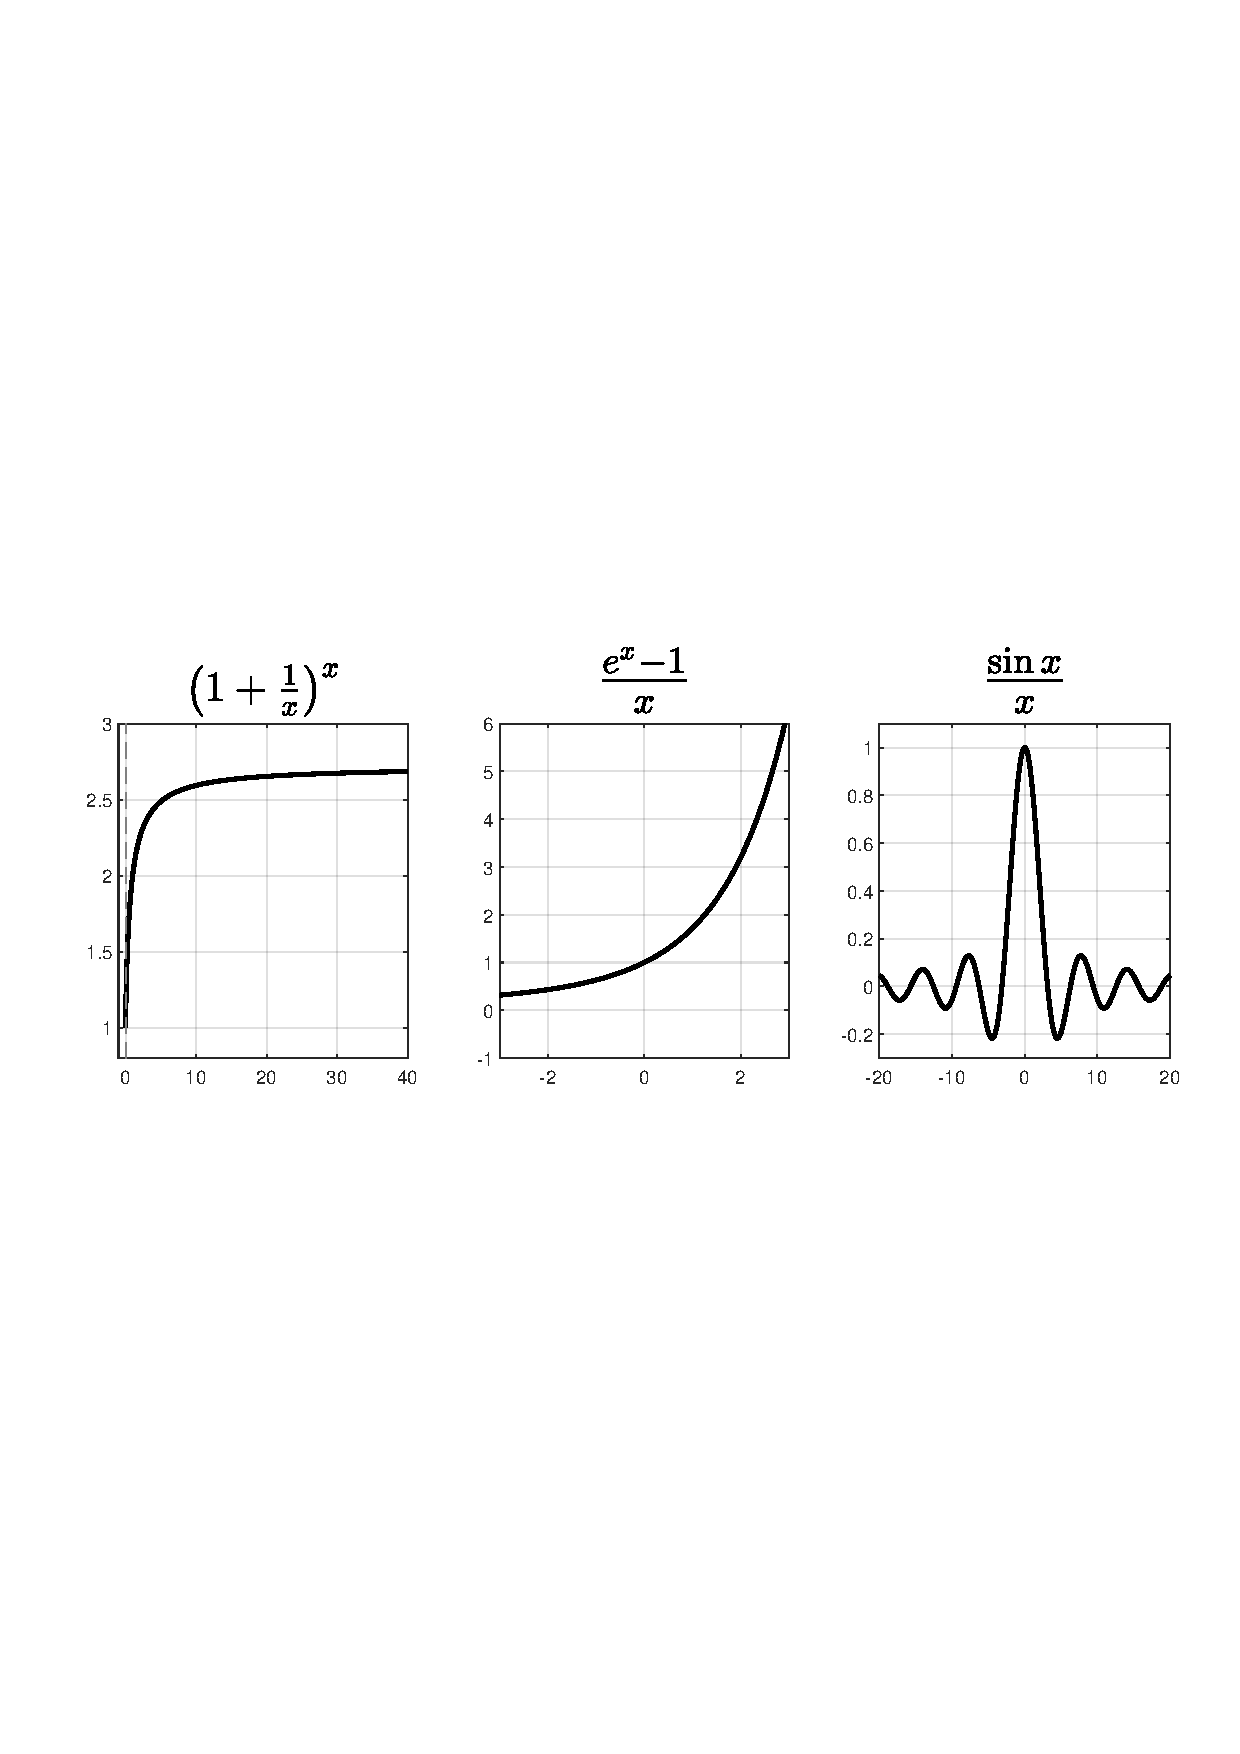
\includegraphics[width=0.8\linewidth]{两个重要极限图像.pdf}
\end{figure}\\

\item 设$ z_1=r_1(\cos\alpha_1 +\i\sin\alpha_1),\ 
z_2=r_2(\cos\alpha_2 +\i\sin\alpha_2) $,那么
\begin{align*}
z_1z_2=\ & r_1(\cos\alpha_1+\i\sin\alpha_1)\cdot r_2(\cos
\alpha_2+\i\sin\alpha_2)\\=\ & (r_1r_2)[(\cos\alpha_1\cos\alpha_2-
\sin\alpha_1\sin\alpha_2)+\i(\sin\alpha_1\cos\alpha_2+
\cos\alpha_1\sin\alpha_2)]\\=\ & (r_1r_2)[\cos(\alpha_1+
\alpha_2)+\i\sin(\alpha_1+\alpha_2)]
\end{align*}
所以,复数乘法的效果是:模相乘,幅角相加。

\item 设$ z=x+\i y=r\cos \alpha+\i r\sin \alpha $,现将$ z $绕原点逆时针旋转$ \theta $角,得到新的复数$ z'=x'+\i y' $,$ z' $的模仍然是$ r $,但幅角变成$ \alpha+\theta $,所以
\begin{gather}\label{坐标旋转公式}
\begin{cases}
    x'=r\cos (\alpha+\theta)=\underbrace{r\cos\alpha}_{x}
    \cos\theta-	\underbrace{r\sin\alpha}_{y}\sin\theta	
    =x\cos\theta-y\sin\theta  \\
    y'=r\sin (\alpha+\theta)=\underbrace{r\sin\alpha}_{y}
    \cos\theta+\underbrace{r\cos\alpha}_{x}\sin\theta
    =x\sin\theta+y\cos\theta
\end{cases} 
\end{gather}
以上两式可实现坐标的旋转。可使用下面的复数乘法辅助记忆坐标旋转公式。
\begin{gather*}
x'+\i y'=(x+\i y)(\cos\theta +\i\sin\theta)
=(x\cos\theta-y\sin\theta)+\i(x\sin\theta+y\cos\theta)
\end{gather*} 
%$ \begin{aligned}
%   \cos\dfrac{\pi}{9}=\dfrac{1}{2}\left(e^{i\dfrac{\pi}{9}}+
%    e^{-i\dfrac{\pi}{9}}\right)=&\ \dfrac{1}{2}\left(\sqrt[3]{e^{i\dfrac{\pi}{3}}}+
%    \sqrt[3]{e^{-i\dfrac{\pi}{3}}}\right)\\
%    =&\ \dfrac{1}{2}\left(\sqrt[3]{\dfrac{1}{2}+
    %    \dfrac{\sqrt{3}}{2}i}+ \sqrt[3]{\dfrac{1}{2}-\dfrac{\sqrt{3}}{2}i}\right)
%    =0.939692\cdots 
%\end{aligned} $
\item 两个单位复数的加减法:(注意使用和差化积公式)
\begin{align*}
    \e^{\i\theta_1}+\e^{\i\theta_2}=&\ (\cos\theta_1+\cos\theta_2)+\i(\sin\theta_1+\sin\theta_2)\\
    =&\ 2\cos\dfrac{\theta_1+\theta_2}{2}\cos\dfrac{\theta_1-\theta_2}{2}+
    2\i\sin\dfrac{\theta_1+\theta_2}{2}\cos\dfrac{\theta_1-\theta_2}{2} \\
    =&\ 2\cos\dfrac{\theta_1-\theta_2}{2}\e^{\i\frac{\theta_1+\theta_2}{2}}  \\
    \e^{\i\theta_1}-\e^{\i\theta_2}=&\ (\cos\theta_1-\cos\theta_2)+\i(\sin\theta_1-\sin\theta_2)\\
    =&\ -2\sin\dfrac{\theta_1+\theta_2}{2}\sin\dfrac{\theta_1-\theta_2}{2}+
    2\i\cos\dfrac{\theta_1+\theta_2}{2}\sin\dfrac{\theta_1-\theta_2}{2} \\
    =&\ 2\sin\dfrac{\theta_1-\theta_2}{2}\e^{\i\frac{\theta_1+\theta_2+\pi}{2}}  
\end{align*}

\end{itemize}

\section{$ n $ 倍角公式}
\begin{itemize}[leftmargin=\inteval{\myitemleftmargin}pt,itemsep=
   \inteval{\myitemitempsep}pt,topsep=\inteval{\myitemtopsep}pt]
\item 利用
\begin{gather}\label{欧拉公式n倍角情形}
    \e^{\i nx}=\cos nx +\i\sin nx=\left(
    \e^{\i x} \right)^n =(\cos x+\i\sin x)^n
\end{gather}
可得$ n $倍角公式。 $ 2\sim 6 $倍角公式如下:
\begin{align*}
    & \sin 2x=2\sin x\cos x \\    
    & \sin 3x=-4 \sin^3 x+ 3\sin x 	  \\
    & \sin 4x=4\cos^3x\sin x-4\cos x\sin^3 x  \\
    & \sin 5x=16\sin^5 x-20\sin^3 x+5 \sin x  \\
    & \sin 6x=6\cos^5 x\sin x-20\cos^3 x\sin^3 x+6\cos x \sin^5 x \\
    \\
    & \cos 2x=2\cos^2 x-1=1-2\sin^2 x=\cos^2 x- \sin^2 x  \\		
    & \cos 3x=4 \cos^3 x- 3\cos x  \\		
    & \cos 4x=8 \cos^4 x- 8\cos^2 x+1  \\		
    & \cos 5x=16\cos^5 x- 20\cos^3 x+5\cos x  \\
    & \cos 6x=32\cos^6 x-48\cos^4 x+ 18\cos^2 x-1 
\end{align*}
$ -4 \sin^3 x+ 3\sin x $(或$ 4 \cos^3 x- 3\cos x $)是关于$ \sin x $(或$ \cos x $)
的三次函数,而且正好没有二次项,这一特性也可以用来求解缺二次项的三次方程。

\item 将余弦的$ n $倍角公式看成关于$ \cos x $的多项式
(被称为第一类切比雪夫多项式),记为$ T_n(u) $,
则$ T_n(\cos x)=\cos nx $,
$ T_0(u)=1,\ T_1(u)=u,\ T_2(u)=2u^2-1,\ T_3(u)=4u^3-3u,\ T_4(u)=8u^4-8u^2+1,\cdots $,
其递推公式为:
\begin{align}\label{车比雪夫多项式递推关系}
    T_{n+1}(u)=2uT_n(u)-T_{n-1}(u)
\end{align}
该递推公式实际上就是:$ \cos(n+1)\theta=2\cos\theta\cos n\theta-
\cos(n-1)\theta $,这是容易验证的。 

% 这个方法把方程的次数弄得太高,放弃。
%\item 在$ n $倍角公式中,令$ x=\dfrac{2\pi}{n} $,可得到
%$\sin(\dfrac{2\pi}{n}),\cos(\dfrac{2\pi}{n}) $所满足的代数方程(被称为分圆方程)。
%考虑五等分圆,$ \cos(5\cdot \dfrac{2\pi}{5})=16\cos^5(\dfrac{2\pi}{5})- 20\cos^3 (\dfrac{2\pi}{5})+
%5\cos \dfrac{2\pi}{5}=1 $,令$ u=\cos \dfrac{2\pi}{5} $,则
%\begin{align*}
%    16u^5-20u^3+5u-1=(u-1)(4u^2+2u-1)^2=0
%\end{align*}
%所以,$ \cos \dfrac{2\pi}{5} $是方程$ 4u^2+2u-1=0 $的一个根。
%
%另外,根据$ T_3(u)-T_2(u)=4u^3-3u-(2u^2-1)=(u-1)(4u^2+2u-1) $,有
%\begin{align*}
%    \cos3x-\cos2x=(\cos x-1)(4\cos^2x+2\cos x-1)=0
%\end{align*}
%显然,$ \dfrac{2\pi}{5} $是方程$ \cos3x-\cos2x=0 $的一个根。解二次方程
%$ 4u^2+2u-1=0 $可得:$ \cos\dfrac{2\pi}{5}=u=\dfrac{\sqrt{5}-1}{4} $. 

\item 考虑5次单位根:
\begin{align*}
    x^5-1=&\ (x-1)(x^4+x^3+x^2+x+1)=(x-1) x^2 \left(x^2+x+1+\frac{1}{x}+\frac{1}{x^2} \right)  \\
    =&\  (x-1) x^2 \left[\left( x+\dfrac{1}{x} \right)^2+ \left( x+\frac{1}{x} \right)-1  \right] \\
    =&\ (x-1) x^2\left[ \left(x+\dfrac{1}{x} \right)-\dfrac{\sqrt{5}-1}{2}  \right] 
    \left[ \left(x+\dfrac{1}{x} \right)+\dfrac{\sqrt{5}+1}{2} \right]   \\
    =&\  (x-1)\left( x^2-\dfrac{\sqrt{5}-1}{2}x+1\right) \left( x^2+\dfrac{\sqrt{5}+1}{2}x+1\right) 
\end{align*}
解方程$  x^2-\dfrac{\sqrt{5}-1}{2}x+1=0 $,可得$ x_{1,2}=\dfrac{\sqrt{5}-1}{4}
\pm \i\dfrac{\sqrt{10+2\sqrt{5}}}{4}=\cos\dfrac{2\pi}{5}\pm \i \sin \dfrac{2\pi}{5} $. 

\item 利用特殊的等腰三角形计算$ \cos\dfrac{2\pi}{5} $:
在三个内角分别为$ 36^{\circ},72^{\circ},72^{\circ}$
的等腰三角形中,连接$ 72^{\circ} $角的顶点和对边中点,
可得一对相似三角形,根据对应边成比例的性质可以得到一个二次方程,
从而求得$ 36^{\circ},72^{\circ},18^{\circ} $的正、余弦值。
\begin{figure}[h]
    \centering
    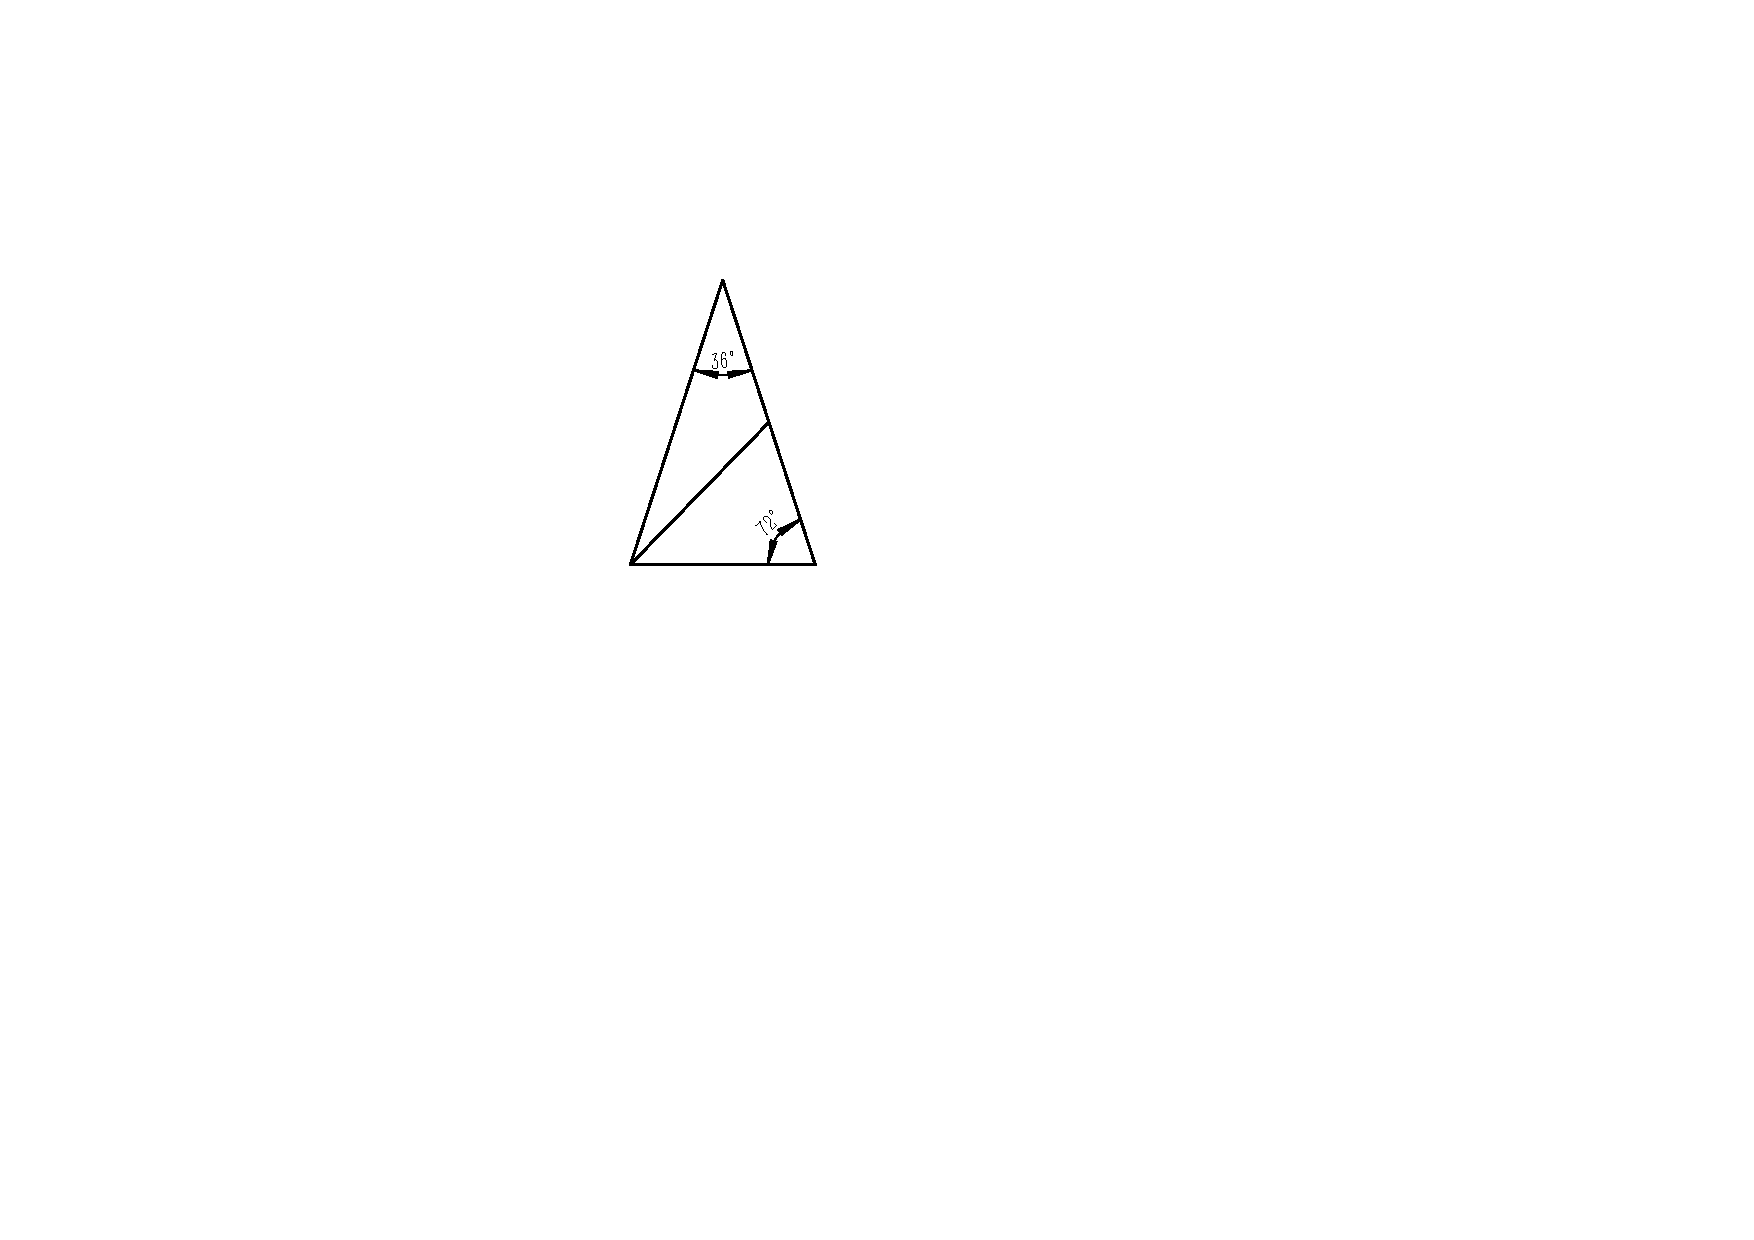
\includegraphics[width=0.2\linewidth]{36度72度三角形}
\end{figure} \\
因为$ 36=3\times 3 \times 2\times 2 $,所以,只要利用二倍角和三倍角公式,
并利用二次方程和三次方程的求根公式,就能得到$ 1^{\circ} $角的
正余弦值的根式表达式。

\item 当$ n $是奇数时有
\begin{gather}\label{两个互补的角的余弦之和为零}
    \cos\dfrac{(n+1)\pi}{2n}+\cos\dfrac{(n-1)\pi}{2n}=0
\end{gather}
上式中令$ n=5 $,有
\begin{gather*}
    \cos\dfrac{3\pi}{5}+\cos\dfrac{2\pi}{5}=0
\end{gather*}
设$ \cos\dfrac{\pi}{5}=x $,利用三倍角和二倍角公式,有
\begin{gather*}
    (4x^3-3x)+(2x^2-1)=0
\end{gather*}
观察到$ x=-1 $是以上3次方程的一个根,故可以因式分解:
\begin{gather*}
    (x+1)(4x^2-2x-1)=0
\end{gather*}
$ \cos\dfrac{\pi}{5}=\dfrac{1+\sqrt{5}}{4} $就是方程
$ 4 x^2-2x-1=0 $的正根。因为$ \cos\dfrac{\pi}{5} $的表达式
只含有二次根式,所以尺规作图可以作出正五边形。\\
类似地,在\eqref{两个互补的角的余弦之和为零}中令$ n=7 $,
设$ \cos\dfrac{\pi}{7}=x $,利用四倍角和三倍角公式,有
\begin{gather*}
    (8x^4-8x^2+1)+(4x^3-3x)=0 \\
    (x+1)(8x^3-4x^2-4x+1)=0
\end{gather*}
利用三次方程的求根公式,就能写出$ \cos\dfrac{\pi}{7} $
的根式表达式\footnote{我经常拿“$ \sin\frac{\pi}{7} $的精确值如何用根式表达?”去测试各个AI聊天机器人,比如ChatGPT、Claude、DeepSeek、文心一言等,几乎没有AI能够(一次性)答对,做得最好的AI,也犯了拿$ \cos\frac{\pi}{7} $的表达式当成$ \sin\frac{\pi}{7} $的表达式的错误。做得差的AI,直接说无法用根式表达,或者给一些错得离谱的等式,连同一个角的正余弦值的平方和为1这种简单公式都用不对。目前没有AI会对它自己给出的根式表达式进行数值计算,再判断是否与直接用某种编程语言的库函数计算$ \sin\frac{\pi}{7} $的值(在浮点误差范围内)相等,很容易出现自信满满地胡说八道的现象。}。该表达式含有三次根式,所以尺规作图无法作出正七边形。\\
在\eqref{两个互补的角的余弦之和为零}中令$ n=17 $,
并记$ \cos\dfrac{\pi}{17}=x $,则
\begin{gather*}
    (256x^9-576x^7+432x^5-120x^3+9x)+(128x^8-256x^6+160x^4-32x^2+1)=0\\
    (x+1)(256x^8-128x^7-448x^6+192x^5+240x^4-80x^3-40x^2+8x+1)=0
\end{gather*}
只要能解出上面的8次方程,就能写出$ \cos\dfrac{\pi}{17} $
的根式表达式。高斯找出了尺寸作图画正17边形的方法\footnote{参见
    https://www.zhihu.com/question/26096850},本质上就是
找到了这个8次方程的根式解,而且这些解都只含有二次根式,
但高斯的解法的出发点并不是
$ \cos\dfrac{9\pi}{17}+\cos\dfrac{8\pi}{17}=0 $,
而是利用了17次单位根的乘法的周期性。

\item 利用$ \cos x=\dfrac{\e^{\i x}+\e^{-\i x}}{2},
\sin x=\dfrac{\e^{\i x}-\e^{-\i x}}{2\i} $可得:$
\cos^n x=\left( \dfrac{\e^{\i x}+\e^{-\i x}}{2}\right)^n,\ 
\sin^n x=\left(\dfrac{\e^{\i x}-\e^{-\i x}}{2\i}\right)^n $,
% 请写出$ \cos^3 x,\cos^4 x,\cdots \sin^3 x,\sin^4 x,\cdots $ 的表达式并总结规律。\\
\begin{align*}
    &  \sin^3 x=\dfrac{1}{4}(-\sin3x+3\sin x)  \\
    &  \cos^3 x=\dfrac{1}{4}( \cos3x+3\cos x)	\\
    &  \sin^4 x=\dfrac{1}{8}(\cos 4x-4\cos 2x+3)  \\
    &  \cos^4 x=\dfrac{1}{8}(\cos 4x+4\cos 2x+3) 
\end{align*}
这种变形的用途之一就是计算积分:$ \int \cos^n x \d x $和$ \int \sin^n x \d x $. 

\end{itemize}

\section{一些连加与连乘公式}
\begin{itemize}[leftmargin=\inteval{\myitemleftmargin}pt,itemsep=
   \inteval{\myitemitempsep}pt,topsep=\inteval{\myitemtopsep}pt]
\item 利用如下两个恒等式可计算$ \sum\limits_{k=1}^{n}\cos kx $
和$ \sum\limits_{k=1}^{n}\sin kx $. 
\begin{align*}
    &\sin\left( n+\dfrac{1}{2}\right) x-\sin\left( n-\dfrac{1}{2}\right) x=2\cos nx\sin \dfrac{x}{2} \\
    &\cos\left( n-\dfrac{1}{2}\right) x-\cos\left( n+\dfrac{1}{2}\right) x=2\sin nx\sin \dfrac{x}{2} 	 		
\end{align*}
将$ n $个这样的式子相加可得:
\begin{align}
    \sum_{k=1}^{n}\cos kx=\dfrac{\sin\left( n+\dfrac{1}{2}\right) x-\sin 
        \dfrac{x}{2}}{2\sin \dfrac{x}{2}} \label{余弦等差连加} \\
    \sum_{k=1}^{n}\sin kx=\dfrac{-\cos\left( n+\dfrac{1}{2}\right) x+\cos 
        \dfrac{x}{2}}{2\sin \dfrac{x}{2}}	\label{正弦等差连加}
\end{align}
这两个求和常被作为数学归纳法的例题。对这两个公式两边同时求导,可以衍生出很多结果。
还可利用欧拉公式计算求和结果,$ \sum\limits_{k=1}^{n}\e^{\i kx}=\dfrac{\e^{\i x}-\e^{\i(n+1)x}}{1-\e^{\i x}} $,
实部就是$ \sum\limits_{k=1}^{n}\cos kx $,虚部就是$ \sum\limits_{k=1}^{n}\sin kx $. 
令$ x=\dfrac{2\pi}{n} $,两个和式均为0,此时$ \cos kx+\i\sin kx $就是1的$ n $次单位根,
它们等间距分布在单位圆上。如果把它们看作一个个的质点,那么它们的重心肯定在原点。

\item 反复使用正弦二倍角公式:
\begin{align*}
    \sin x =&\ 2\sin\dfrac{x}{2} \cos\dfrac{x}{2} \\
    =&\ 2^2 \sin\dfrac{x}{4} \cos\dfrac{x}{4}  \cos\dfrac{x}{2} \\
    =&\  \cdots \\
    =&\  2^n \sin\dfrac{x}{2^n}\cos\dfrac{x}{2^n} \cdots \cos\dfrac{x}{4}\cos\dfrac{x}{2}     
\end{align*}
所以
\begin{align}\label{余弦等比连乘}
    \cos\dfrac{x}{2} \cos\dfrac{x}{4}\cdots  \cos\dfrac{x}{2^n}
    =\dfrac{\sin x}{2^n \sin\dfrac{x}{2^n}}
\end{align}
例如,令$ n=3,x=\dfrac{8\pi}{9} $,则
\begin{align*}
    \cos\dfrac{\pi}{9}\cos\dfrac{2\pi}{9}\cos\dfrac{4\pi}{9}
    =\dfrac{\sin\dfrac{8\pi}{9}}{8\sin\dfrac{\pi}{9}}=\dfrac{1}{8}
\end{align*}

\item 根据等式$ \cos\left(2\cdot \dfrac{\theta}{2^{n+1}}\right)=
2\cos^2\left(\dfrac{\theta}{2^{n+1}}\right)-1 $,
如果记$ a_n=\cos\left(\dfrac{\theta}{2^n}\right) $,那么
\begin{gather*}
    a_{n+1}^2=\dfrac{1}{2}a_n+\dfrac{1}{2},\q a_{n+1}=\sqrt{\dfrac{a_n+1}{2}}
\end{gather*}
以后面对这一递推关系,就知道了其通项公式。再做代换$ a_{n}=\dfrac{1}{2}b_n $,
就能得到另一种常见变体:
\begin{gather*}
    \dfrac{1}{4}b_{n+1}^2=\dfrac{1}{4}b_n+\dfrac{1}{2},\q 
    b_{n+1}^2=b_n+2,\q b_{n+1}=\sqrt{b_n+2}
\end{gather*}

\item $ (1-z)(1+z+z^2+\cdots +z^{n-1})=1-z^{n} $,令$ z_k=\e^{\i\frac{2k\pi}{n}},
\ k=1,2,\cdots,n-1 $,则$ z_k^n=\e^{\i\cdot 2k\pi}=1 $,$ z_k $是方程
$ 1+z+z^2+\cdots +z^{n-1}=0 $的$ n-1 $个根,所以,
\begin{gather*}
    (z-z_1)(z-z_2)\cdots(z-z_{n-1})=1+z+z^2+\cdots +z^{n-1}
\end{gather*}
令$ z=1 $可得:
\begin{gather*}
    (1-z_1)(1-z_2)\cdots(1-z_{n-1})=1+1+1+\cdots +1=n
\end{gather*}
两边同时取模:
\begin{gather}\label{1-zk取模}
    |1-z_1||1-z_2|\cdots|1-z_{n-1}|=n
\end{gather}
另外,
\begin{gather*}
    1-z_k=1-\cos\left(\dfrac{2k\pi}{n} \right)-
            \i\sin\left(\dfrac{2k\pi}{n} \right) \\ 
    |1-z_k|=\sqrt{\left[1-\cos\left(\dfrac{2k\pi}{n} \right) \right]^2+
   \sin^2 \left(\dfrac{2k\pi}{n} \right) }=2\sin\left(\dfrac{k\pi}{n}\right)
\end{gather*}
于是(\ref{1-zk取模})式成为:
\begin{align}\label{正弦等差连乘}
    2^{n-1}\sin\left(\dfrac{\pi}{n} \right)\sin\left(\dfrac{2\pi}{n} \right)\cdots
    \sin\left(\dfrac{(n-1)\pi}{n} \right)=n
\end{align}
更一般的结果为:
\begin{align}\label{一般正弦等差连乘}
    2^{n-1}\sin(x)\sin\left(x+\dfrac{\pi}{n} \right)\sin\left(x+\dfrac{2\pi}{n} \right)\cdots
    \sin\left(x+\dfrac{(n-1)\pi}{n} \right)=\sin(nx)
\end{align}
在(\ref{一般正弦等差连乘})式中令$ x \to 0 $,并利用极限$ \lim\limits_{x\to 0}\dfrac{\sin nx}{\sin x}=n $,就能得到
(\ref{正弦等差连乘})式。把(\ref{一般正弦等差连乘})式中的$ x $换成$ x+\dfrac{\pi}{2} $,有:
\begin{align}\label{余弦等差连乘}
    2^{n-1}\cos(x)\cos\left(x+\dfrac{\pi}{n} \right)\cos\left(x+\dfrac{2\pi}{n}
    \right)\cdots \cos\left(x+\dfrac{(n-1)\pi}{n} \right) 
    = \sin\left( nx+\dfrac{n\pi}{2}\right) 
\end{align}

\item 因为$ \tan(x_1-x_2)=\dfrac{\tan x_1-\tan x_2}{
    1+\tan x_1 \tan x_2} $,所以$ \tan x_1 \tan x_2=\dfrac{
    \tan x_1-\tan x_2}{\tan(x_1-x_2)}-1 $,进一步地,
\begin{align*}
    & \tan x\tan 2x+\tan 2x\tan 3x+\cdots +
    \tan (n-1)x\tan nx \\
    =&\ \dfrac{1}{\tan x}\left[(\tan 2x-\tan x)+
    (\tan 3x-\tan 2x)+\cdots +(\tan nx-\tan (n-1)x)\right]
    -(n-1)	\\ =&\  \dfrac{1}{\tan x}\left( \tan nx-
    \tan x\right)-(n-1) \\ =&\  \dfrac{\tan nx}{\tan x}-n
\end{align*}

\end{itemize}

\section{三角形中的等式与不等式}
\begin{itemize}[leftmargin=\inteval{\myitemleftmargin}pt,itemsep=
   \inteval{\myitemitempsep}pt,topsep=\inteval{\myitemtopsep}pt]
\item $ \Delta ABC $中的恒等式($ A+B+C=\pi $)
\begin{align} 
    &\sin A +\sin B +\sin C =4\cos\Big(\dfrac{A}{2}\Big)
    \cos\Big(\dfrac{B}{2}\Big)\cos\Big(\dfrac{C}{2}\Big) \label{三角恒等式1} \\
    &\sin2A +\sin2B +\sin2C =4\sin A  \sin B \sin C \label{三角恒等式2}\\
    &\cos A +\cos B +\cos C =1+4\sin\Big(\dfrac{A}{2}\Big)
    \sin\Big(\dfrac{B}{2}\Big)\sin\Big(\dfrac{C}{2}\Big) \label{三角恒等式3} \\
    &\cos2A +\cos2B +\cos2C =-1-4\cos A\cos B \cos C \label{三角恒等式4} \\	
    &\cos^2A+\cos^2B+\cos^2C =1-2\cos A\cos B\cos C \label{三角恒等式5} \\ 
    &\sin^2A+\sin^2B+\sin^2C =2+2\cos A\cos B\cos C \label{三角恒等式6} \\
    &\tan A+\tan B +\tan C =\tan A \tan B\tan C \label{三角恒等式7}\\
    &\cot A\cot B+\cot B \cot C+\cot A\cot C=1 \label{三角恒等式8}\\
    &\tan\Big(\dfrac{A}{2}\Big)\tan\Big(\dfrac{B}{2}\Big)+
    \tan\Big(\dfrac{B}{2}\Big)\tan\Big(\dfrac{C}{2}\Big)+
    \tan\Big(\dfrac{A}{2}\Big)\tan\Big(\dfrac{C}{2}\Big)=1 \label{三角恒等式-最后}
\end{align}

\item 从左到右证明(\ref{三角恒等式1})式,使用和差化积公式:
\begin{align*}
    & (\sin A +\sin B) +\sin C  \\
    =&\  2\sin\left(\dfrac{A+B}{2}\right)\cos\left(\dfrac{A-B}{2}\right)+\sin(A+B) \\    
    =&\  2\sin\left(\dfrac{A+B}{2}\right)\cos\left(\dfrac{A-B}{2}\right)+
    2\sin\left(\dfrac{A+B}{2}\right)\cos\left(\dfrac{A+B}{2}\right) \\
    =&\  2\sin\left(\dfrac{A+B}{2}\right)\cdot 2\cos\left(\dfrac{A}{2}\right)\cos\left(\dfrac{B}{2}\right) \\
    =&\  4\cos\left(\dfrac{C}{2}\right)\cos\left(\dfrac{A}{2}\right)\cos\left(\dfrac{B}{2}\right)
\end{align*}
\item 从右到左证明(\ref{三角恒等式1})式,
\begin{align*}
    & 4\cos\left(\dfrac{A}{2}\right)\cos\left(\dfrac{B}{2}\right)\sin\left(\dfrac{A+B}{2}\right) \\
    =&\  4\cos\left(\dfrac{A}{2}\right)\cos\left(\dfrac{B}{2}\right) \left[\sin\left(\dfrac{A}{2}\right) \cos\left(\dfrac{B}{2}\right)+\cos\left(\dfrac{A}{2}\right) \sin\left(\dfrac{B}{2}\right) \right] \\
    =&\  4\cos\left(\dfrac{A}{2}\right)\sin\left(\dfrac{A}{2}\right)\cos^2\left(\dfrac{B}{2}\right)+
    4\cos\left(\dfrac{B}{2}\right)\sin\left(\dfrac{B}{2}\right)\cos^2\left(\dfrac{A}{2}\right)\\
    =&\  \sin A (\cos B+1)+\sin B(\cos A +1) \\
    =&\  \sin A +\sin B + \sin(A+B)
\end{align*}
以上方法同样适用于(\ref{三角恒等式2}),(\ref{三角恒等式3}),(\ref{三角恒等式4}).
由(\ref{三角恒等式4})式可以导出(\ref{三角恒等式5})式,
由(\ref{三角恒等式5})式可以导出(\ref{三角恒等式6})式。
由(\ref{三角恒等式6})式可知$ \cos A\cos B\cos C >-1 $,
由(\ref{三角恒等式3})式可知$ \cos A+\cos B+\cos C >1 $.  

\item 由$ \tan(A+B)=\dfrac{\tan A+\tan B}{1-\tan A\tan B}=
\tan(\pi-C)=-\tan C $可得到(\ref{三角恒等式7})式,
(\ref{三角恒等式7})式两边同除$ \tan A \tan B\tan C $可得到(\ref{三角恒等式8})式。
由$ \tan\Big(\dfrac{A}{2}+\dfrac{B}{2}\Big)=\dfrac{\tan \dfrac{A}{2}+
    \tan \dfrac{B}{2}}{1-\tan \dfrac{A}{2}\tan \dfrac{B}{2}}
=\tan\Big(\dfrac{\pi}{2}-\dfrac{C}{2}\Big)=\dfrac{1}{\tan \dfrac{C}{2}} $
可得到(\ref{三角恒等式-最后})式。

\item 对任意$ \Delta ABC $,有如下不等式成立:
\begin{gather}
    0<\sin A +\sin B +\sin C \leq \frac{3\sqrt{3}}{2} \label{sinA+sinB+sinC}\\    
    0<\sin A \sin B \sin C \leq \frac{3\sqrt{3}}{8} \label{sinAsinBsinC}\\
    1<\cos A +\cos B +\cos C \leq \frac{3}{2} \label{cosA+cosB+cosC}\\
    -1<\cos A\cos B\cos C \leq \frac{1}{8} \label{cosAcosBcosC}
\end{gather}
右侧不等号中的等号均在$ A=B=C=\dfrac{\pi}{3} $时取得,左侧则是至少一个角趋于0时的极限
(剩余两个角可能趋于$ 0 $和$ \pi $,也可能都趋于$ \dfrac{\pi}{2} $).

\item (\ref{sinA+sinB+sinC})式左侧不等式显然成立,现证明右侧。\\
\textbf{方法一}\ 利用正弦函数$ y=\sin x $在$ [0,\pi] $上的凹凸性
(不等式(\ref{琴森不等式})):
\begin{gather*}
    \sin A +\sin B +\sin C \leq 3\sin \dfrac{A+B+C}{3}=\dfrac{3\sqrt{3}}{2}
\end{gather*}
\textbf{方法二}\ 考虑$ y=\sin x $在$ \Big(\dfrac{\pi}{3},\dfrac{\sqrt{3}}{2}
\Big) $处的切线$ y=\dfrac{1}{2}\Big(x-\dfrac{\pi}{3}\Big)+\dfrac{\sqrt{3}}{2} $,
$ \forall x\in [0,\pi] $,有$ \sin x\leq \dfrac{1}{2}\Big(x-\dfrac{\pi}{3}\Big)
+\dfrac{\sqrt{3}}{2} $,所以,
\begin{gather*}
    \sin A +\sin B +\sin C \leq \dfrac{1}{2}\Big(A+B+C-3\cdot\dfrac{\pi}{3}\Big)
    +3\cdot\dfrac{\sqrt{3}}{2}=\dfrac{3\sqrt{3}}{2}
\end{gather*}
\textbf{方法三}\ 利用均值不等式(\ref{完整的均值不等式})、(\ref{三角恒等式6})式、
(\ref{cosAcosBcosC})式:
\begin{align*}
    \sin A +\sin B +\sin C \leq &\ \sqrt{3(\sin^2A+\sin^2B+\sin^2C)} \\
    =&\ \sqrt{3(2+2\cos A\cos B\cos C)}\leq \sqrt{3\left(2+2\cdot 
        \dfrac{1}{8}\right)}=\dfrac{3\sqrt{3}}{2}
\end{align*}

\item (\ref{sinAsinBsinC})式左侧不等式显然成立,现证明右侧。利用均值不等式
(\ref{完整的均值不等式}):
\begin{gather}
    \sin A \sin B \sin C \leq \left(\dfrac{\sin A +\sin B +\sin C}{3} \right)^3
    \leq \left(\dfrac{\sqrt{3}}{2}\right)^3=\dfrac{3\sqrt{3}}{8}
    \label{三个正弦和不等式-小于}
\end{gather}

\item 证明(\ref{cosA+cosB+cosC})式。\\
\textbf{方法一}\ 利用(\ref{三角恒等式3})式、均值不等式和正弦函数的凹凸性:
\begin{align}
    \cos A +\cos B +\cos C =&\ 1+4\sin\Big(\dfrac{A}{2}\Big)
    \sin\Big(\dfrac{B}{2}\Big)\sin\Big(\dfrac{C}{2}\Big)\qquad (>1) \nonumber \\
    \leq &\ 1+4\left[\dfrac{\sin(\frac{A}{2})+
        \sin(\frac{B}{2})+\sin(\frac{C}{2})}{3}\right]^3 \nonumber \\
    \leq &\ 1+ 4\left(\sin \dfrac{\frac{A}{2}+\frac{B}{2}+\frac{C}{2}}{3}\right)^3=
    1+4\left(\dfrac{1}{2}\right)^3=\dfrac{3}{2} \label{三个余弦和不等式-小于}
\end{align}
\textbf{方法二}\ 考虑$ y=\cos x $在$ \Big(\dfrac{\pi}{3},\dfrac{1}{2}
\Big) $处的切线$ y=-\dfrac{\sqrt{3}}{2}\Big(x-\dfrac{\pi}{3}\Big)+\dfrac{1}{2} $,
$ \forall x\in [0,\pi] $,有$ \cos x\leq -\dfrac{\sqrt{3}}{2}\Big(x-
\dfrac{\pi}{3}\Big)+\dfrac{1}{2} $,所以,
\begin{gather*}
    \cos A +\cos B +\cos C \leq -\dfrac{\sqrt{3}}{2}\Big(A+B+C-3\cdot
    \dfrac{\pi}{3}\Big)+3\cdot\dfrac{1}{2}=\dfrac{3}{2}
\end{gather*}

\item 对于(\ref{cosAcosBcosC})式,因为$ |\cos A\cos B\cos C|<1 $,
所以$ \cos A\cos B\cos C>-1 $,左侧成立。现证明(\ref{cosAcosBcosC})式右侧成立。\\
\textbf{方法一}\ 利用均值不等式:
\begin{gather*}
    \cos A \cos B \cos C \leq \left(\dfrac{\cos A +\cos B +\cos C}{3} \right)^3
    \leq \left(\dfrac{1}{2}\right)^3=\dfrac{1}{8}
\end{gather*}
\textbf{方法二}\ 利用(\ref{三角恒等式5})式和均值不等式,
\begin{align*}
    1-2\cos A\cos B\cos C=\cos^2A+\cos^2B+\cos^2C \geq 3(\cos A\cos B\cos C)^{2/3}
\end{align*}
记$ t=(\cos A\cos B\cos C)^{1/3} $,那么 $ 2t^3+3t^2-1= (2t-1)(t+1)^2 \leq 0 $,
于是$ t\leq \dfrac{1}{2} $,$ \cos A\cos B \cos C=t^3\leq \dfrac{1}{8} $.  

\item 当$ x\in\Big(0,\dfrac{\pi}{2}\Big) $时,
$ \sin x>\dfrac{2}{\pi}x $,$ \cos x>1-\dfrac{2}{\pi}x $.
\begin{figure}[!h]  % sinx_Great_2x_pi.m
    \centering
    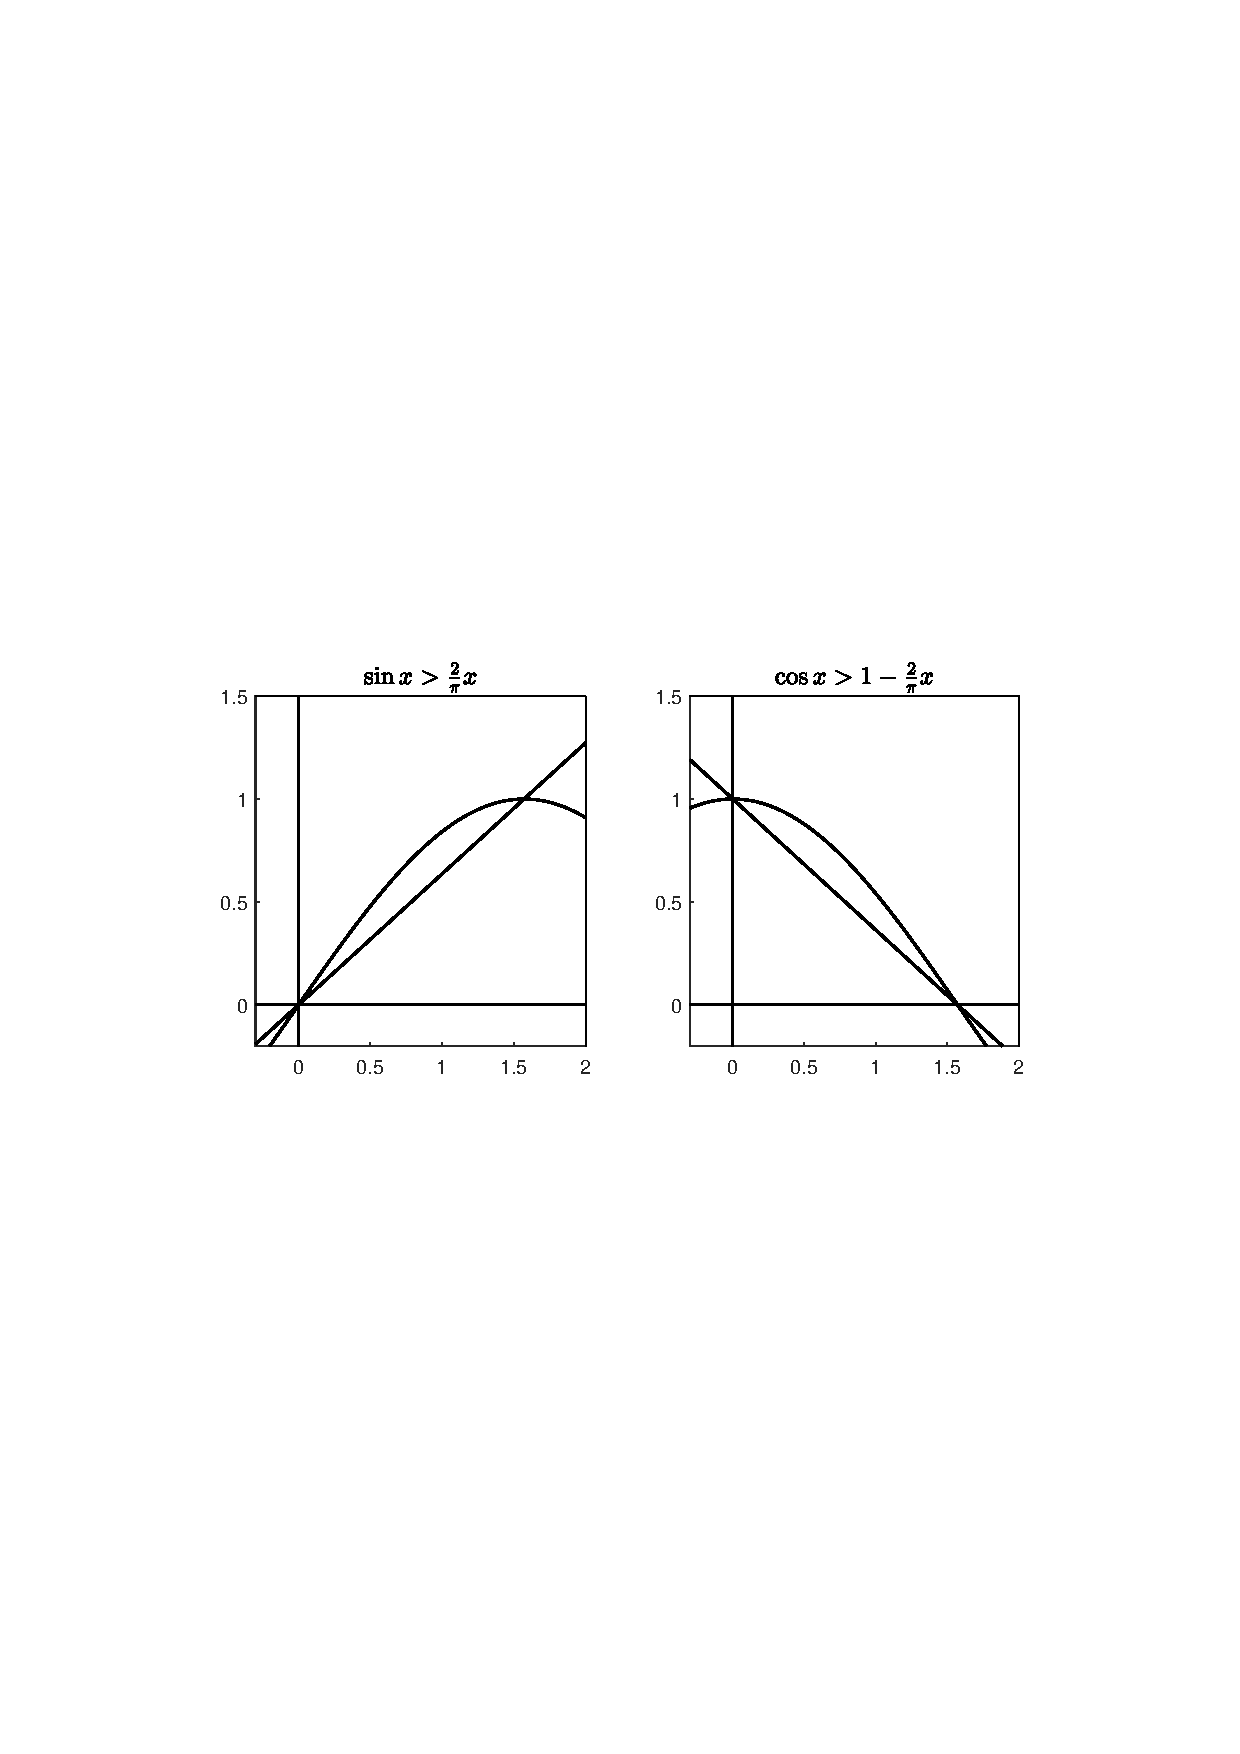
\includegraphics[width=0.7\linewidth]{sinx大于2x_pi}
\end{figure} \\
对于锐角三角形$ ABC $,有
\begin{align*}
    \sin A +\sin B +\sin C &>\dfrac{2}{\pi}(A+B+C)=2 \\
    \cos A +\cos B +\cos C &>3-\dfrac{2}{\pi}(A+B+C)=1
\end{align*}

\item 若$ \Delta ABC $是钝角三角形,那么$ \tan A+\tan B +\tan C =
\tan A \tan B\tan C <0 $.\\
若$ \Delta ABC $是锐角三角形,那么
\begin{gather*}
    \tan A+\tan B +\tan C =\tan A \tan B\tan C \leq \left(
    \dfrac{\tan A+\tan B +\tan C}{3}\right)^3
\end{gather*}
于是
\begin{gather*}
    \tan A+\tan B +\tan C\geq 3\sqrt{3}
\end{gather*}
也可以从正切函数的凹凸性来理解上式,
\begin{gather*}
    \tan A+\tan B +\tan C\geq 3\tan\dfrac{A+B+C}{3}=3\sqrt{3}
\end{gather*}
或者考虑$ y=\tan x $在$ \Big(\dfrac{\pi}{3},\sqrt{3}\Big) $
处的切线$ y=4\Big(x-\dfrac{\pi}{3}\Big)+\sqrt{3} $,
$ \forall x\in \Big[0,\dfrac{\pi}{2}\Big) $,有$ \tan x\geq 
4\Big(x-\dfrac{\pi}{3}\Big)+\sqrt{3} $,所以,
\begin{gather*}
    \tan A +\tan B +\tan C \geq 4\Big(A+B+C-3\cdot\dfrac{\pi}{3}\Big)
    +3\sqrt{3}=3\sqrt{3}
\end{gather*}


\end{itemize}

\section{例题}
\begin{enumerate}[label={【\textbf{例\thechapter.\arabic*}】},
 leftmargin=\inteval{\myenumleftmargin}pt,
 itemsep=\inteval{\myenumitempsep}pt,
 itemindent=\inteval{\myenumitemindent}pt]
\item (2021,上海春季高考)已知$ \theta>0 $,存在实数$ \varphi $,
使得对任意 $ n\in \mathbf{N}^{+} $,$ \cos(n\theta+\varphi)
<\dfrac{\sqrt{3}}{2} $,求$ \theta $的最小值。
\begin{figure}[!ht]
    \centering
    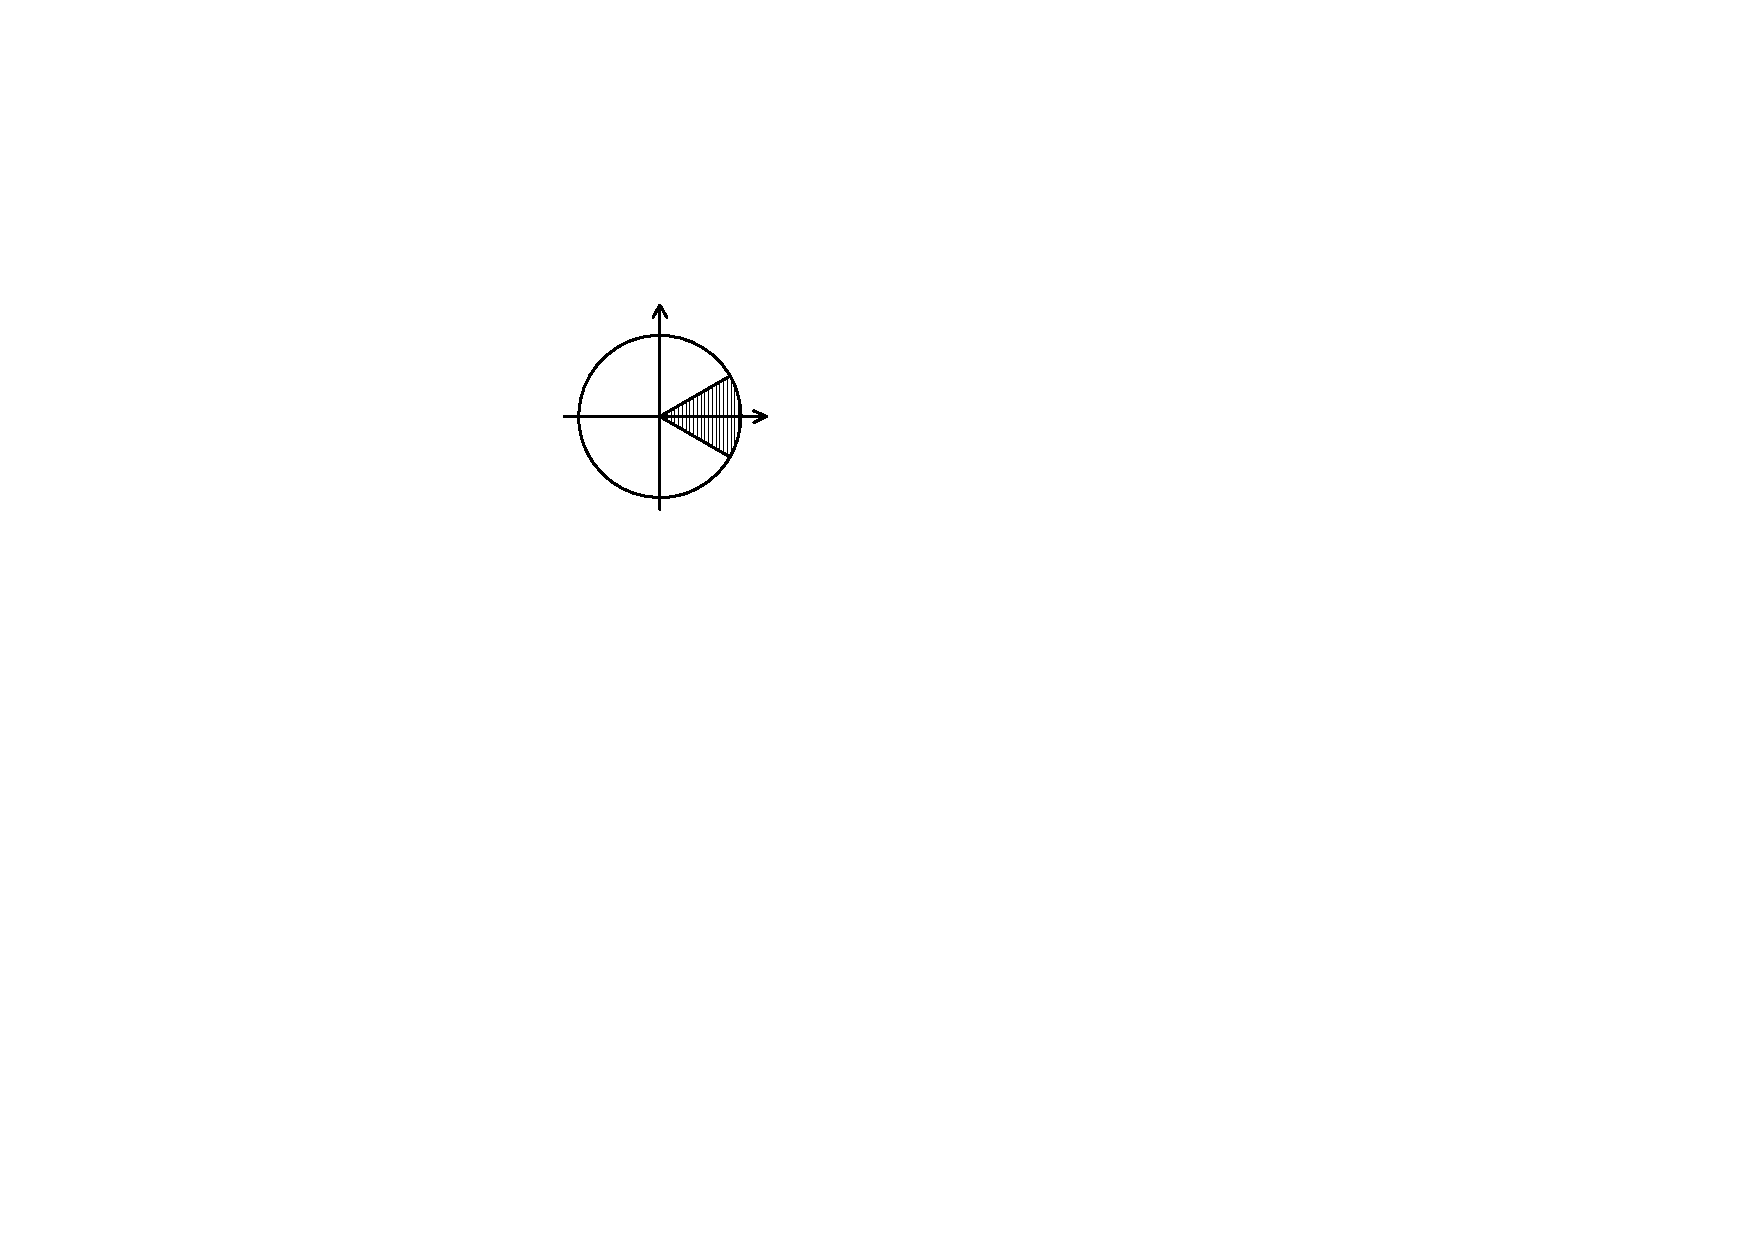
\includegraphics[width=0.3\linewidth]{2021上海春季高考-角度问题}
\end{figure} \\
\textbf{解}\ 题目的意思是,可以选择一个合适的$ \varphi $作为初始值,
然后每次逆时针旋转$ \theta $角(步长为$ \theta $),无论转多少次,
始终不会落在圆心角为$ \dfrac{\pi}{3} $的阴影区域中,
那么必有$ \theta>\dfrac{\pi}{3} $. 
这是因为,当$ n $足够大时,总会需要跨过阴影区域,步长太小,当然跨不过去。
另外,$ \theta $必须是$ 2\pi $的$ N $分之一,$ N\in \textbf{N}^+ $.
否则,转有限次后始终无法恰好回到初始位置,总会错开一些,最终必然会进入
阴影区域。举个例子,取$ \theta=1.1>\dfrac{\pi}{3},\ \varphi=-0.55 $,
当$ n=6 $时,$ n\theta+\varphi=6.05\in\left(\dfrac{11\pi}{6},
2\pi\right) $,进入了阴影区域。

综上所述,$ \dfrac{2\pi}{N}>\dfrac{\pi}{3},\ N=5 $,
$ \theta $的最小值是$ \dfrac{2\pi}{5} $. 

\item 求$ \arctan \dfrac{1}{2}+\arctan \dfrac{1}{3} $和$ \arctan 1+
\arctan 2+\arctan 3 $. \\
\textbf{方法一}\ $ \arctan x+\arctan y=\arctan\dfrac{x+y}{1-xy} $,
\begin{gather*}
    \arctan \dfrac{1}{2}+ \arctan\dfrac{1}{3}=\arctan\dfrac{\dfrac{1}{2}
        +\dfrac{1}{3}}{1-\dfrac{1}{2}\times \dfrac{1}{3}}=\arctan 1=\dfrac{\pi}{4}
\end{gather*}
更一般地,当$ x\in [0,1] $时,$ \arctan x+\arctan \dfrac{1-x}{1+x}=\dfrac{\pi}{4} $. 
\begin{align*}
    (\arctan 1+\arctan 2)+\arctan 3 &=\arctan\dfrac{1+2}{1-1\times 2}
    +\arctan3 \\ &= (\pi-\arctan 3)+\arctan 3=\pi
\end{align*}
\textbf{方法二}\ 复数相乘的效果是:模相乘,角相加。\\
取$ a=2+\i,\ b=3+\i $,$ a,b $的幅角分别为$ \arctan 
\dfrac{1}{2},\arctan \dfrac{1}{3} $. \\ $ ab=(2+\i)(3+\i)=5+5\i $,
它的幅角为$ \dfrac{\pi}{4} $. \\
$ z_1=1+\i,\ z_2=1+2\i,\ z_3=1+3\i,\ z_1z_2z_3=-10 $,所以$ z_1,z_2,z_3 $
的幅角之和为$ \pi $. 

\item (2020,清华强基计划) 求$ \sum\limits_{k=1}^{\infty}\arctan\dfrac{2}{k^2} $. 
\\ \textbf{解}\ $ \arctan x-\arctan y=\arctan\dfrac{x-y}{1+xy} $,
\begin{align*}
    \sum_{k=1}^{\infty}\arctan\dfrac{2}{k^2} 
    =&\ \sum_{k=1}^{\infty}\arctan\dfrac{(k+1)-(k-1)}{1+(k+1)(k-1)} \\
    =&\ \sum_{k=1}^{\infty}\left[
    \arctan(k+1)-\arctan(k-1) \right]\\
    =&\ 2\arctan(+\infty)-\arctan1-\arctan0=
    \dfrac{3\pi}{4}
\end{align*}
类似地,$ \arctan\dfrac{1}{2k^2}=\arctan\dfrac{1}{2k-1}-
\arctan\dfrac{1}{2k+1} $. 

\item 求$ \dfrac{2\cos7.5^{\circ}-\sin22.5^{\circ}}{\cos 22.5^{\circ}} $的值。\\
\textbf{解}\ 
\begin{align*}
    \dfrac{2\cos7.5^{\circ}-\sin22.5^{\circ}}{\cos 22.5^{\circ}}=&\ 
    \dfrac{2\cos(30^{\circ}-22.5^{\circ})-\sin22.5^{\circ}}{\cos 22.5^{\circ}}\\ 
    =&\ \dfrac{2(\dfrac{\sqrt{3}}{2}\cos22.5^{\circ}+\dfrac{1}{2}\sin22.5^{\circ})
        -\sin22.5^{\circ}}{\cos 22.5^{\circ}} = \sqrt{3}
\end{align*} 

\item $ \sin(\sin x),\ \sin(\cos x),\ \cos(\cos x),\ \cos(\sin x) $
的周期都是\underline{$\quad 2\pi \quad $}. $ \sin(\sin x),\ 
\sin(\cos x) $的值域是\underline{$\quad [-\sin 1,\sin 1] \quad$}. 
$ \cos(\cos x),\ \cos(\sin x) $的值域是\underline{$\quad
    [\cos 1,1] \quad $}. 

\item 用反证法证明:$ \tan 1^{\circ} $不是有理数。\\
\textbf{证}\ 假设$ \tan 1^{\circ} $是有理数,那么
\begin{align*}
    \tan 2^{\circ}&=\dfrac{2\tan 1^{\circ}}{1-\tan^2 1^{\circ}} \in \textbf{Q}\\
    \tan 3^{\circ}&=\tan (1^{\circ}+2^{\circ})=\dfrac{\tan 1^{\circ}
        +\tan 2^{\circ}}{1-\tan 1^{\circ}\cdot \tan 2^{\circ}} \in \textbf{Q} \\
    &\vdots \\
    \tan 15^{\circ}&=\tan (1^{\circ}+14^{\circ})=\dfrac{\tan 1^{\circ}+
        \tan 14^{\circ}}{1-\tan 1^{\circ}\cdot \tan 14^{\circ}} \in \textbf{Q}
\end{align*}
以上都是有理数,但$ \tan 15^{\circ}=\dfrac{\sqrt{6}-\sqrt{2}}{\sqrt{6}+\sqrt{2}}
=2-\sqrt{3} $是无理数,这就产生了矛盾,所以原命题成立。(若不熟悉$ 15^{\circ} $的正切值,
也可以递推到$ \tan 30^{\circ} $,与$ \tan 30^{\circ}=\dfrac{\sqrt{3}}{3} $是无理数矛盾。)\\
\textbf{注}:$ \tan 75^{\circ}=2+\sqrt{3} $. 

\item 证明:$ \sin\left( \dfrac{1}{x}\right)  $不是周期函数。\\
\textbf{证}\ 用反证法,假设$ \sin\left( \dfrac{1}{x}\right)  $是周期函数,$ T $是它的一个正周期,那么
$ \sin\left( \dfrac{1}{x}\right)= \sin\left( \dfrac{1}{x+T}\right) $对任意$ x\neq 0,-T $成立,
显然,对$ x=1 $成立,即$ \sin\left( \dfrac{1}{1}\right)= \sin\left( \dfrac{1}{1+T}\right) $,
然而,根据正弦函数在区间$ [0,\dfrac{\pi}{2}] $上单调递增的性质,应该有$ \sin\left( \dfrac{1}{1}\right)> 
\sin\left( \dfrac{1}{1+T}\right) $,与前面的等式矛盾,
所以$ \sin\left( \dfrac{1}{x}\right)  $不是周期函数。

\item 证明:$ \sin(\sqrt{x})$不是周期函数。 \\
\textbf{证}\ 用反证法,假设$ \sin(\sqrt{x}) $的最小正周期是$ T $,那么$ \sin(\sqrt{x})=
\sin(\sqrt{x+T})=\sin(\sqrt{x+2T}) $,令$ x=0 $可得:
$ \sin(0)=\sin(\sqrt{T})=\sin(\sqrt{2T})=0 $,
于是存在正整数$ m,n $满足:$ \sqrt{T}=m\pi,\sqrt{2T}=n\pi $,两式相除可得:
$ \sqrt{2}=\dfrac{n}{m} $,这与$ \sqrt{2} $是无理数相矛盾。

\item $ ^* $ 证明:$ \sin(x^2) $不是周期函数。\\
\textbf{证}\ 用反证法,假设$ \sin(x^2) $的最小正周期是$ T $,
那么$ \sin(x^2)=\sin\left[(x+T)^2\right] $,
令$ x=0 $可得:$ \sin(0)=\sin(T^2)=0,\ T^2=m\pi,\ T=\sqrt{m\pi} $. 
再令$ x=\sqrt{2m\pi} $可得:$ \sin(2m\pi)=\sin\left[(
\sqrt{2m\pi}+\sqrt{m\pi})^2\right]=\sin\left[(3+2\sqrt{2})m\pi\right]=0 $,
于是$ (3+2\sqrt{2})m\pi=n\pi,\ 3+2\sqrt{2}=\dfrac{n}{m} $,$ 3+2\sqrt{2} $是无理数,
$ \dfrac{n}{m} $是有理数,这就产生了矛盾。

\item $ \sin\Big(\dfrac{1}{x}\Big),\sin(\sqrt{x}),\sin(x^2)$均不是周期函数,
它们的零点都不是等间距分布的。这3个函数可分别看成$\sin\left(\dfrac{1}{x^2}
\cdot x\right),\sin\left(\dfrac{1}{\sqrt{x}}\cdot x\right), 
\sin\left(x\cdot x\right)$,其中的$ \dfrac{1}{x^2},\dfrac{1}{\sqrt{x}},x $
可看成它们各自的$ \omega $,所以,随着$ |x| $增大,
$\sin\left(\dfrac{1}{x^2} \cdot x\right), 
\sin\left(\dfrac{1}{\sqrt{x}}\cdot x\right)$频率降低,曲线变得更加稀疏。
而$ \sin(x\cdot x) $的频率提高,曲线变得更加密集。
\begin{figure}[h] % SinNonPeriodicTrigonometricFunction.m
    \centering
    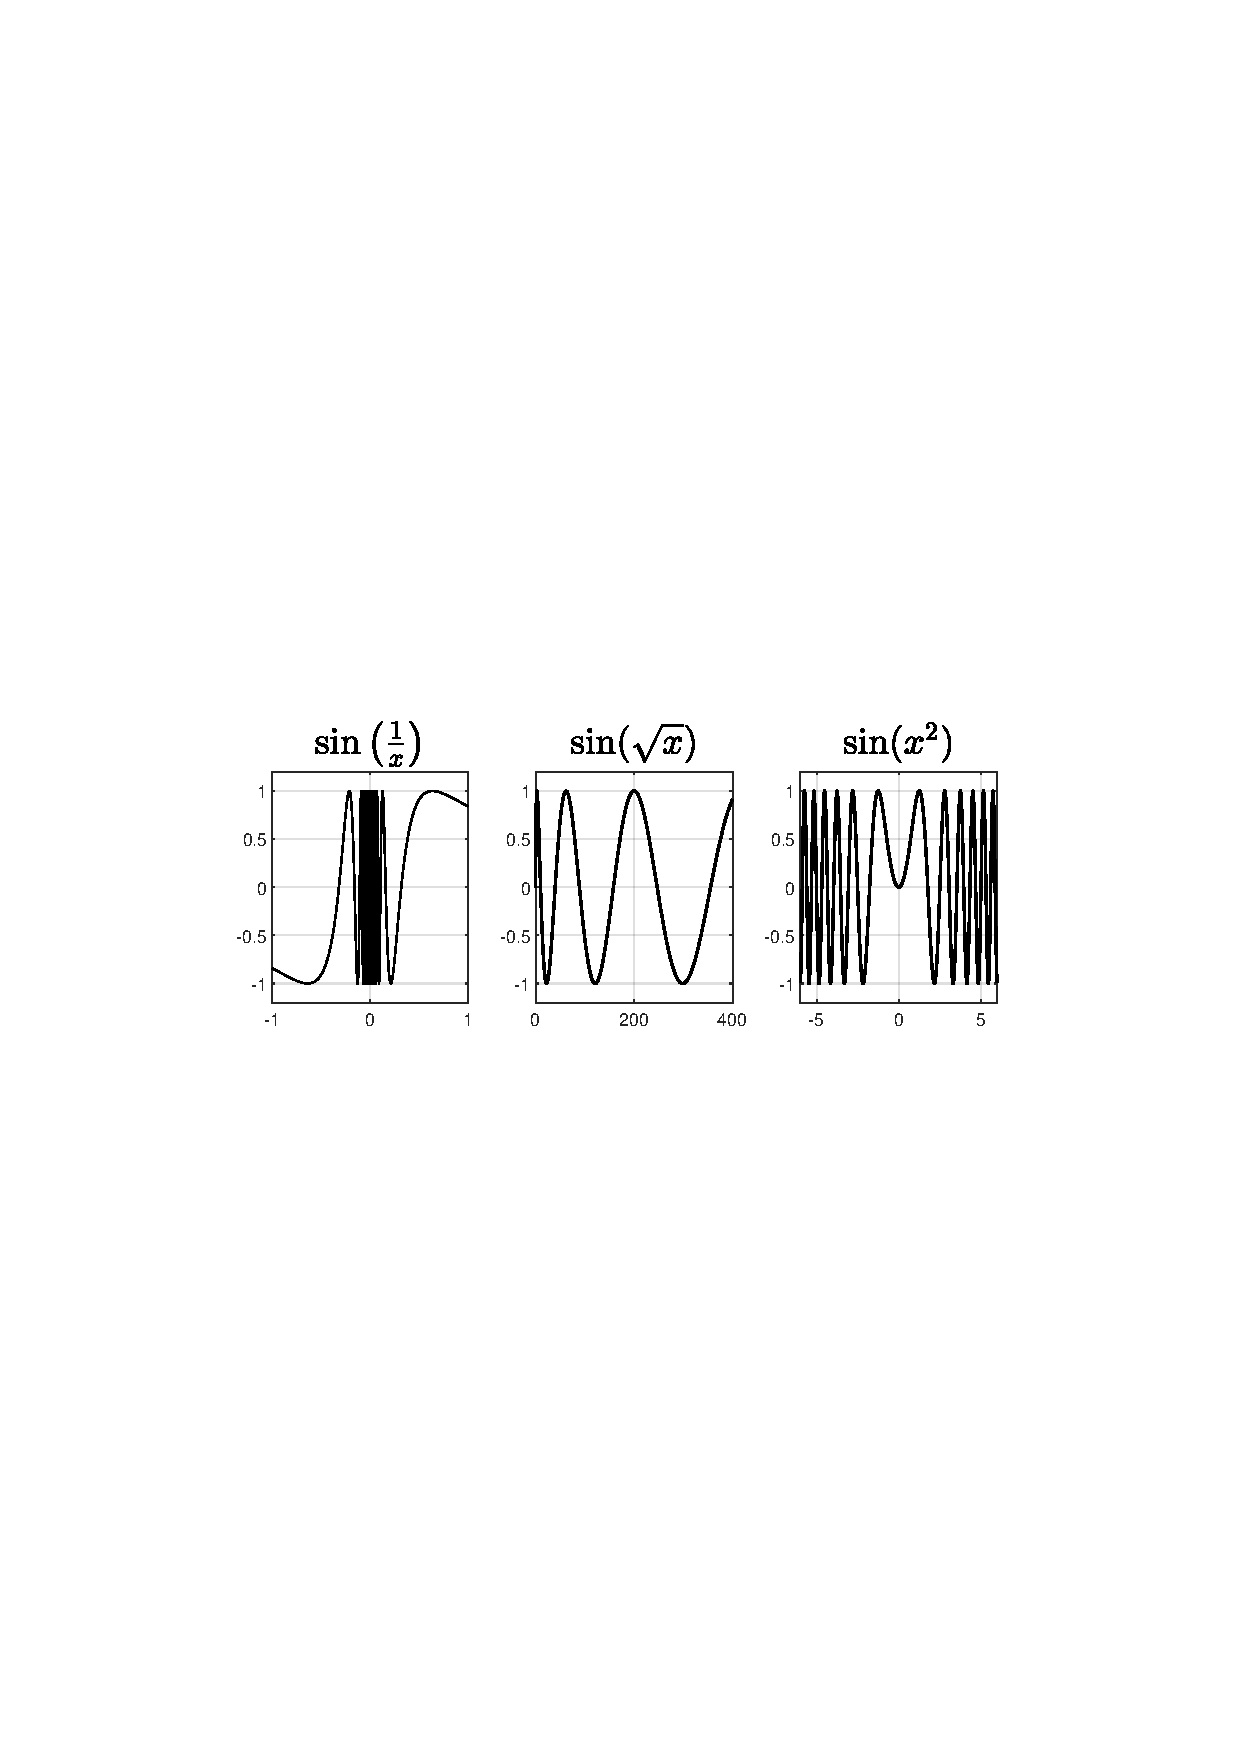
\includegraphics[width=0.7\linewidth]{三个sin括号内变化的非周期函数}
\end{figure} 

\item $ x\sin x,\dfrac{\sin x}{x},\dfrac{x}{\sin x} $均不是周期函数。 \\
\begin{figure}[h] % SinNonPeriodicTrigonometricFunction.m
    \centering
    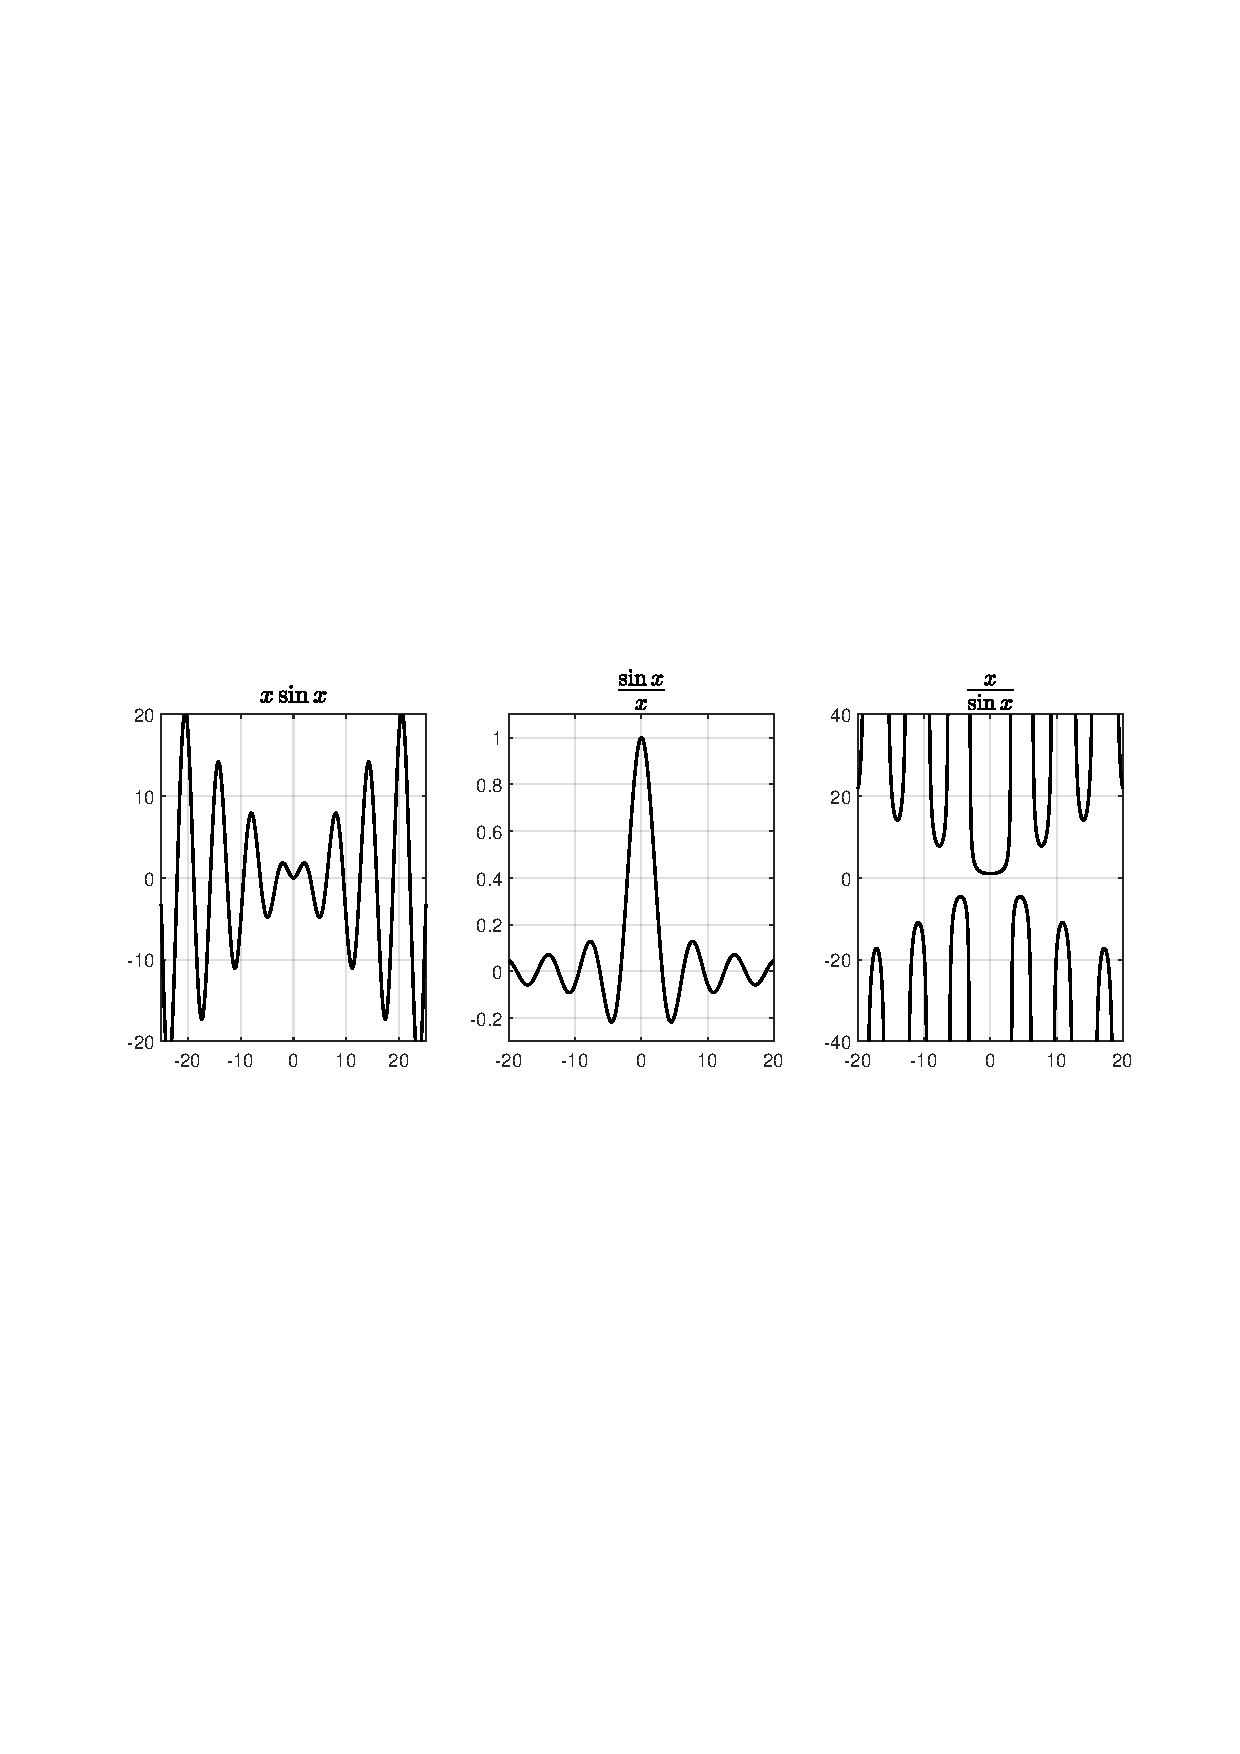
\includegraphics[width=0.7\linewidth]{三个乘除型非周期函数}
\end{figure}

% ShangHai2015.m
\item (2015,上海高考)对于定义域为$ \mathbf{R} $的函数$ g(x) $,
若存在正的常数$ T $,使得$ \cos g(x) $是以$ T $为周期的函数,
则称$ g(x) $为余弦周期函数,且称$ T $为其余弦周期。已知 $ f(x) $
是以 $ T $ 为余弦周期的余弦周期函数,其值域为 $ \mathbf{R} $.
设 $ f(x) $ 单调递增,$ f(0)=0,\ f(T)=4\pi $. \\
(1)验证$ g(x)=x+\sin\dfrac{x}{3} $是以$ 6\pi $为周期的余弦周期函数;\\
(2)设$ a<b $,证明对任意$ c\in[f(a),f(b)] $,存在 $ x_{0}\in[a,b] $,
使得 $ f(x_{0})=c $ ;\\
(3)证明:“$ u_{0} $ 为方程 $ \cos f(x)=1 $在$ [0,T] $上的解”
的充要条件是“ $ u_{0}+T $为方程$ \cos f(x)=1 $在区间$ [T,2T] $
上的解”,并证明:$\forall x\in[0,T] $,都有$ f(x+T)=f(x)+f(T) $ .\\
\textbf{解}\ (1)略 (2)由连续函数的介值定理或零点存在定理可得,略。 \\
(3) 充要条件证明略,重点关注$ f(x+T)=f(x)+f(T) $. \\
%\textbf{方法一}\ 容易验证,当$ x=0 $和$ T $时,结论成立。
%$ \cos f(2T)=\cos f(T)=\cos4\pi=1 $,因$ f(x) $单调递增,
%故$ f(2T)> f(T)=4\pi $,($ f(2T) $不可能等于$ 4\pi $,否则
%$ f(x) $在$ [T,2T] $上恒等于$ 4\pi $,不可能是余弦周期函数。),
%所以,$ f(2T)=2k_1\pi,\ k_1\in \textbf{N},\ k_1\geq 3 $. \\
%\mycircled{1} 若$ k_1=3 $,则$ f(2T)=6\pi $,由(2)知存在$ x_0\in
%(0,T) $,使得$ f(x_0)=2\pi\in(0,4\pi) $,
%\begin{gather*}
%    \cos f(x_{0}+T)=\cos f(x_{0})=\cos2\pi=1\q \Rightarrow\q
%    f(x_{0}+T)=2k_{2}\pi,\ k_{2}\in\mathbf{Z}
%\end{gather*}
%$ f(T)<f(x_{0}+T)<f(2T) $,
%$4\pi<2k_2\pi<6\pi \Rightarrow\ 2<k_{2}<3$,矛盾;\\
%\mycircled{2} 若$k_{1}\geqslant 5,\ f(2T)\geqslant 10\pi$,
%则存在$ T<x_{1}<x_{2}<2T $,使得$ f(x_{1})=6\pi,\ f(x_{2})=8\pi $.
%则$ T,x_{1},x_{2},2T $为$ \cos f(x)=1 $在$[T,2T]$上的4个解,
%由“充要条件”可得,$ \cos f(x)=1 $在$[0,T]$上也有4个解。
%但$\cos f(x)=1$在$[0,T]$上只有$f(x)=0,2\pi,4\pi $这3个解,矛盾;\\
%\mycircled{3} 当$k_{1}=4$时,$f(2T)=8\pi=f(T)+f(T)$ ;
%当$x\in(0,T)$时,$f(x)\in(0,4\pi)$,考查方程$\cos f(x)=c$在$(0,T)$上的解,
%设其解为$f(x_{1}),f(x_{2}),\cdots,f(x_{n}) $,
%$ (x_{1}<x_{2}<\cdots<x_{n},\ 3\leq n\leq 4) $,
%则$f(x_{1}+T),f(x_{2}+T),\cdots,f(x_{n}+T)$为方程$\cos f(x)=c$在$(T,2T)$上的解。
%又$f(x_i+T)\in(4\pi,8\pi)$,而$f(x_{1})+4\pi,f(x_{2})+4\pi,\cdots,f(x_{n})+4\pi\in(4\pi,8\pi)$为方程$\cos f(x)=c$在$(T,2T)$上的解,所以
%\begin{align*}
% f(x_{i}+T)=f(x_{i})+4\pi=f(x_{i})+f(T)
%\end{align*}
%
%综上所述,对任意$x\in[0,T]$,都有$f(x+T)=f(x)+f(T)$.\\
%\textbf{方法二}\ 
因为$ \cos f(x+T)=\cos f(x) $,所以必有
\begin{gather} \label{2015上海解法二1}
    f(x+T)= f(x) +2k\pi,\q k\in \textbf{N}^+ 
\end{gather}
或者
\begin{gather}\label{2015上海解法二2}
    f(x+T)= 2k\pi-f(x),\q k\in \textbf{N}^+
\end{gather}
因为(\ref{2015上海解法二2})式左侧关于$ x $单调递增,
右侧关于$ x $单调递减,矛盾,所以(\ref{2015上海解法二2})式
不可能成立。

在(\ref{2015上海解法二1})式中令$ x=0 $可得:$ f(T)=f(0)+2k\pi $,
所以$ k=2 $,
\begin{gather*}
    f(x+T)=f(x)+4\pi=f(x)+f(T)
\end{gather*}

是否可能出现如下情况呢?比如存在$ t\in(0,T) $,
存在$ x_1\in(0,t),x_2\in (t,T) $,使得
\begin{align}
    f(x_1+T) &= f(x_1) +2k_1\pi,\q k_1\in \textbf{N}^+ \label{2015上海解法二3}  \\
    f(x_2+T) &= f(x_2) +2k_2\pi,\q k_2\in \textbf{N}^+ \label{2015上海解法二4}
\end{align}
其中$ k_1\neq k_2 $. 
回答是不可能。假如(\ref{2015上海解法二3}),(\ref{2015上海解法二4})
两式都成立,那么在$ x=t+T $处,$ f(x) $的左右极限不相等。
又因为$ f(x) $是单调递增的,说明$ f(x) $在$ x=t+T $处出现了一个
向上的跳跃(或称“间断”),此时,$ f(x) $的值域就达不到\textbf{R},
与题意矛盾。证毕。\\
\textbf{注}:$ f(x+T)=f(x)+f(T) $与正比例函数的函数方程
$ f(x+y)=f(x)+f(y) $很相似,但我们并不能得出$ f(x) $
在$ (0,T) $上是正比例函数的结论,因为$ T $是固定的,而
$ y $是任意的。只能得出如下结论:
$ f(x) $在$ (T,2T) $上的图像是由$ f(x) $在$ (0,T) $
上的图像向右平移$ T $,再向上平移$ f(T)=2k\pi $得到的。
其它区间类似。比如$ f(x) $的一种可能的图像如下:
\begin{figure}[!ht]
    \centering
    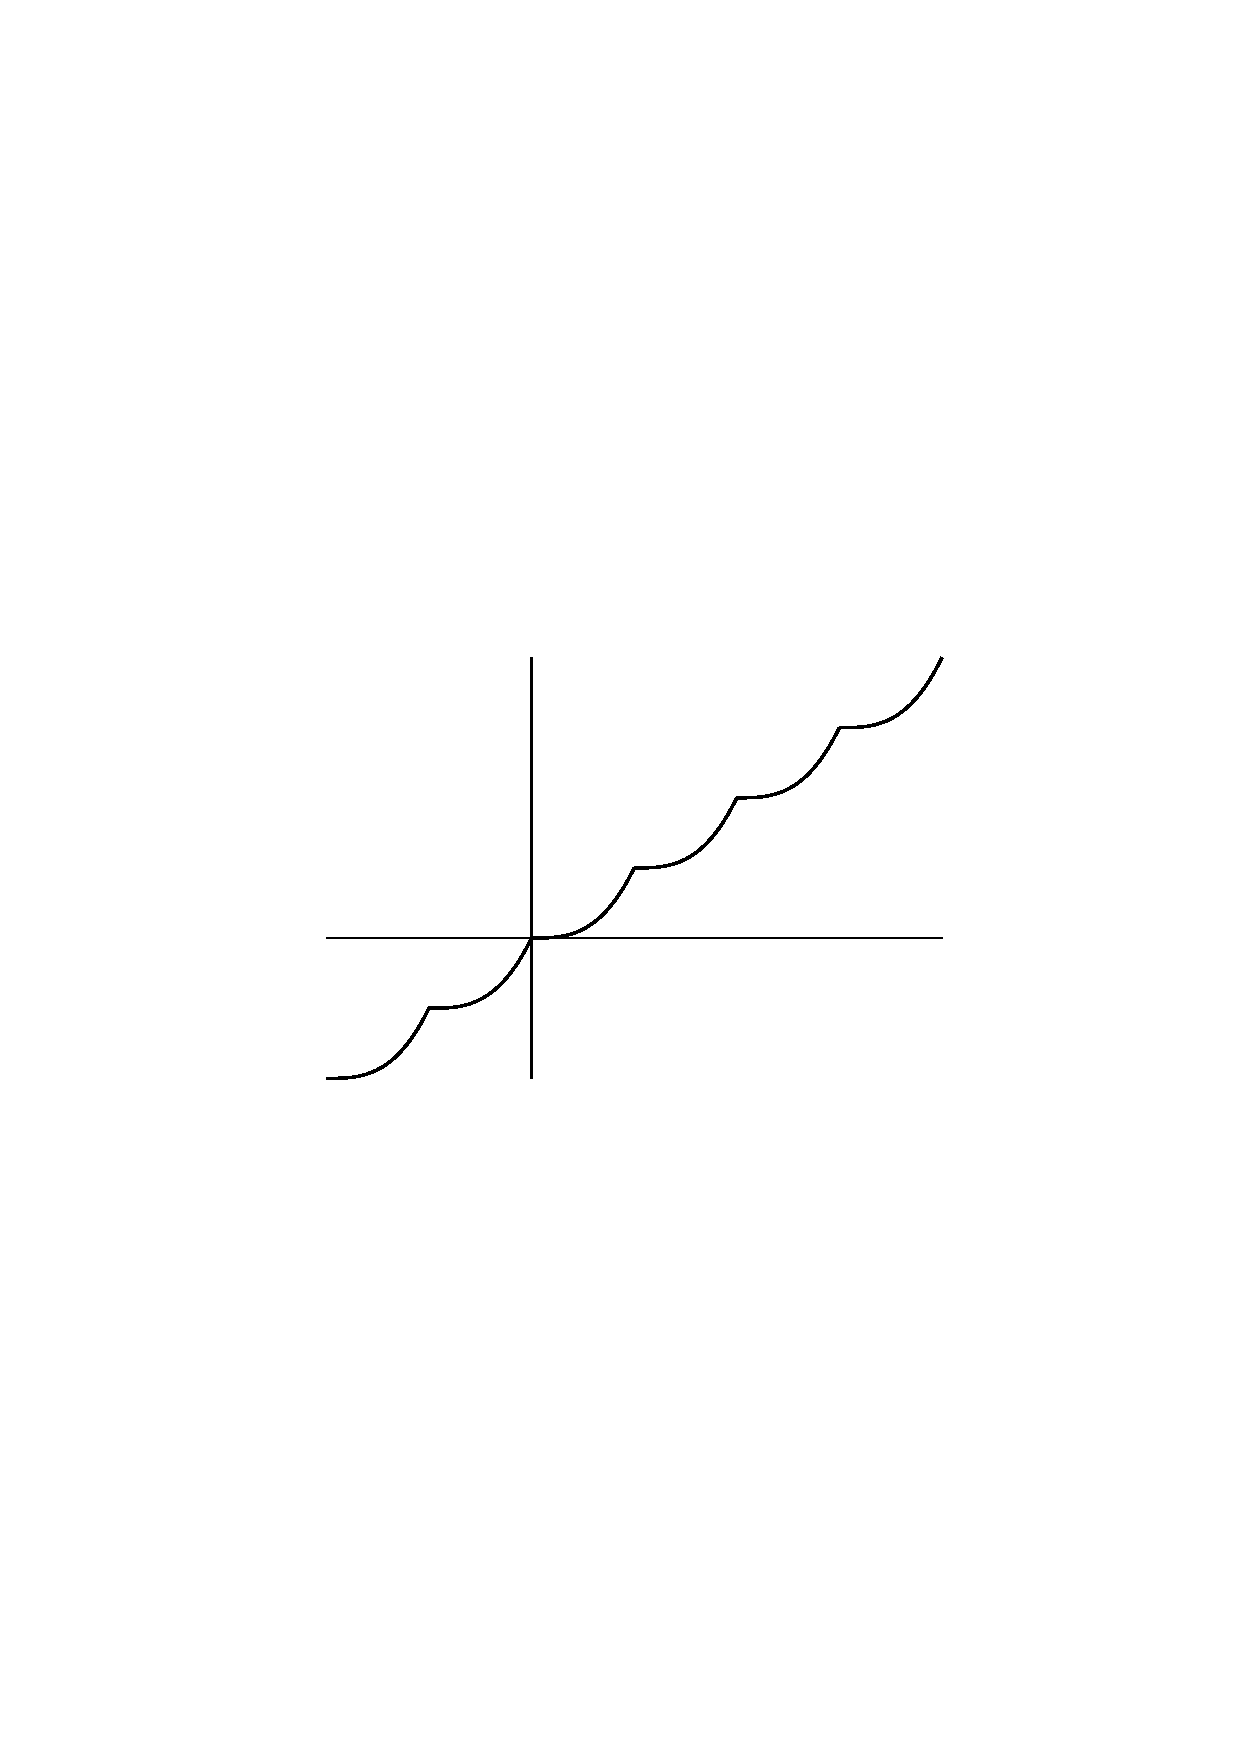
\includegraphics[width=0.4\linewidth]{2015上海高考}
\end{figure}

\item 用求根公式计算$ x^3-3x^2+4x-6=0 $的实根,然后借助计算器用二分法求实根。\\
\textbf{解}\ 作变换$ x=t+1 $,则原方程变为$ t^3+t-4=0,\ p=1,\ q=-4,\ 
\Delta=\dfrac{q^2}{4}+\dfrac{p^3}{27}=\dfrac{109}{27} $,原方程实根为:
\begin{align*}
    x =\sqrt[3]{2+\sqrt{\dfrac{109}{27}}}+\sqrt[3]{2-\sqrt{\dfrac{109}{27}}}+1  
    =&\  \dfrac{\sqrt[3]{54+3\sqrt{327}}}{3}+\dfrac{\sqrt[3]{54-3\sqrt{327}}}{3}+1 \\
    =&\  \dfrac{\sqrt[3]{54+3\sqrt{327}}}{3}-\dfrac{1}{\sqrt[3]{54+3\sqrt{327}}}+1
\end{align*}

\item 求复系数二次方程$ (1+\i)x^2+2\i x+3=0 $的两个根。\\
\textbf{方法一}\ $ \Delta=4\i^2-12(1+\i)=-16-12\i $,设$ \Delta=(a+b\i)^2 $,那么
$ \begin{cases}
    a^2-b^2 =&\ -16 \\
    2ab =&\ -12
\end{cases} $ ,解得
$ \begin{cases}
    a=&\ \sqrt{2} \\
    b=&\ -3\sqrt{2}
\end{cases} $或
$ \begin{cases}
    a=&\ -\sqrt{2} \\
    b=&\ 3\sqrt{2}
\end{cases} $. 
于是
\begin{gather*}
    x_{1,2}=\dfrac{-2\i\pm (\sqrt{2}-3\sqrt{2})\i}{2(1+\i)}=-\dfrac{1}{2}
    -\dfrac{1}{2}\i\pm \Big(\dfrac{\sqrt{2}}{2}+\sqrt{2} \i\Big)
\end{gather*}
注意,此时的两个复数根不是共轭复数,这与实系数二次方程不一样。

\item 去掉$ \sqrt{6+2\sqrt{5}} $ 和 $ \sqrt{2+\sqrt{3}} $ 
的外层根号。\\
\textbf{解}\ 设$ 6+2\sqrt{5}=(a+b\sqrt{5})^2=(a^2+5b^2)+2ab\sqrt{5}$,
那么
$ \begin{cases}
    a^2+5b^2 =&\ 6 \\
    2ab =&\ 2
\end{cases} $ ,解得
$ a=\pm 1,\ b=\pm 1 $,即$ \sqrt{6+2\sqrt{5}}=1+\sqrt{5} $. \\
设 $ 2+\sqrt{3}=(c+d\sqrt{3})^2=(c^2+3d^2)+
2cd\sqrt{3} $,解得$ c=\pm \dfrac{\sqrt{6}}{2},\ d=\pm \dfrac{\sqrt{6}}{6} $,
即$  \sqrt{2+\sqrt{3}} = \dfrac{\sqrt{6}+\sqrt{2}}{2} $.  \\
\\
更一般地,设$ A+B\sqrt{C}=(a+b\sqrt{C})^2=(a^2+b^2C)+2ab\sqrt{C} $,因为
$ A=a^2+b^2C \geq 2\sqrt{a^2b^2C} =2|ab|\sqrt{C}=|B|\sqrt{C}>0 $,所以
$ A\geq |B|\sqrt{C} $是可以去掉外层根号的必要不充分条件。
比如$ \sqrt{1+\sqrt{5}} $,$ \sqrt{-2+\sqrt{5}} $不满足必要条件,
均无法去掉外层根号。即使满足了必要条件,比如$ \sqrt{10+2\sqrt{5}} $,
$ \sqrt{2+\sqrt{2}} $,也无法去掉外层根号,这两者分别等于$ \sqrt{5+2\sqrt{5}}+
\sqrt{5-2\sqrt{5}} $,$ \dfrac{1}{2}\bigl(\sqrt{4+2\sqrt{2}}+
\sqrt{4-2\sqrt{2}}\bigr) $. 

\item 求无理系数二次方程$ \sqrt{3}\, x^2+4x-2=0 $的两个根。\\
\textbf{解}\ $ \Delta=16+8\sqrt{3}=(2+2\sqrt{3})^2 $,
$ x_1=1-\dfrac{\sqrt{3}}{3} $,$ x_2=-1-\sqrt{3} $. \\
\textbf{注}:如果多项式$ f(x) $的所有系数均为实数,当$ a+b\i $是$ f(x)=0 $的根时,
$ a-b\i $也是$ f(x)=0 $的根。如果多项式$ f(x) $的所有系数均为有理数,
当$ a+b\sqrt{C} $是$ f(x)=0 $的根时,$ a-b\sqrt{C} $也是$ f(x)=0 $的根。

\item 定义集合$ S=\{m+n\sqrt{3}|m^2-3n^2=1,m,n\in \textbf{Z}\} $,
求证:若$ x,\ y\in S $,则$ \dfrac{1}{x}\in S,\ xy \in S,\ x+y\notin S $. \\
\textbf{证}\ 设$ x=a+b\sqrt{3},\ y=c+d\sqrt{3},\ a,b,c,d\in \textbf{Z} $,
则$ \dfrac{1}{x}=\dfrac{1}{a+b\sqrt{3}}=a-b\sqrt{3} $,因为$ a^2-3(-b)^2=1 $,
所以$ \dfrac{1}{x}\in S $. 容易看出,$ \pm a \pm b\sqrt{3} $均属于$ S $. 
\begin{align*}
    xy=(a+b\sqrt{3})(c+d\sqrt{3})=&\  (ac+3bd)+(ad+bc)\sqrt{3} \\
    (ac+3bd)^2-3(ad+bc)^2 =&\  a^2c^2+6abcd+9b^2d^2-3a^2d^2-6abcd-3b^2c^2 \\
    =&\  a^2(c^2-3d^2)-3b^2(c^2-3d^2)=a^2-3b^2=1 
\end{align*}
所以,$ xy\in S $.
\begin{align*}
    & x+y=(a+c)+(b+d)\sqrt{3} \\
    & (a+c)^2-3(b+d)^2=(a^2-3b^2)+(c^2-3d^2)+2(ac-3bd)=2(1+ac-3bd)\neq 1
\end{align*}
所以,$ x+y\notin S $. 令$ x=y $,可得$ x^2\in S $,进一步有$ x^k\in S\ 
(k\in \textbf{N}^+) $. \\
\textbf{注1}:满足$ m^2-3n^2=1 $的整数$ m,n $在全体整数中的占比并不大,
首先,$ m $不可能是3的倍数。因为,如果$ m=3K $,
那么$ m^2-3n^2=3(3K^2-n^2)=1 $,这显然是不可能的。
在$ |m|<1000 $的范围内,只有如下五组:
\begin{gather*}
    2^2-3\cdot 1^2=1,\quad  7^2-3\cdot 4^2=1,\quad  26^2-3\cdot 15^2=1, \\
    97^2-3\cdot 56^2=1,\quad 362^2-3\cdot 209^2=1
\end{gather*}
事实上,$ (2\pm\sqrt{3})^2=7\pm 4\sqrt{3} $,
$ (2\pm\sqrt{3})^3=26\pm 15\sqrt{3} $,
$ (2\pm\sqrt{3})^4=97\pm 56\sqrt{3} $,
$ (2\pm \sqrt{3})^5=362\pm 209\sqrt{3} $. 
根据二项式定理,
\begin{gather*}
    \begin{cases}
        m_k &=\dfrac{1}{2}[(2+\sqrt{3})^k+(2-\sqrt{3})^k] \\ 
        n_k &=\dfrac{1}{2\sqrt{3}}[(2+\sqrt{3})^k-(2-\sqrt{3})^k]    
    \end{cases} , \q  k\in \textbf{N}^+
\end{gather*}
便是方程$ m^2-3n^2=1 $的通解
\footnote{形如$ m^2-dn^2=\pm 1 $ 的方程被称为佩尔(Pell)方程
(实际上,此类方程由费马首先进行了深入研究,拉格朗日给出了解决方案,
但被欧拉误记为佩尔提出,并写入他的著作中,然后该称呼沿用至今。),其中,$ d>0 $
且不含平方因子。从上面的例子可以看出,只要找到佩尔方程的一组整数解,就能生成无数组解。
但佩尔方程不一定有整数解,比如$ m^2-34n^2=-1 $无整数解。形如$ Am^2-Bn^2=C $的方程
被称为广义Pell方程,比如$ 3m^2-2n^2=1 $的整数解有$ m=1,n=1;\ m=9,n=11;\ m=89,n=109;\cdots $,(\ref{双曲线的有理参数化-nt})式对此类问题有帮助,一些参考文献如下:\\
$ \diamond $ 史保怀,李小雪. 广义Pell方程Ax2-By2=4的通解公式[J]. 纯粹数学与应用数学, 2014, 30(5):6.\\
$ \diamond $ 杨克仁,徐研. 广义Pell方程及其应用[J]. 数学研究, 1995, 28(3):4.}。
由(\ref{二阶线性递推数列韦达定理})式可知,数列$ m_k $满足递推关系:
\begin{align}\label{佩尔方程4-1递推}
    m_{k+2}=4m_{k+1}-m_k
\end{align}
$ n_k $也满足同样的递推关系。递推关系(\ref{佩尔方程4-1递推})与
(\ref{分式与二阶线性等价递推})式和(\ref{1988IMO递推数列})式一样。
\begin{gather*}
    \dfrac{m_k}{n_k}=\sqrt{3}\cdot \dfrac{(2+\sqrt{3})^k+
        (2-\sqrt{3})^k}{(2+\sqrt{3})^k-(2-\sqrt{3})^k}
\end{gather*}
$ \lim\limits_{k\to\infty} \dfrac{m_k}{n_k}=\sqrt{3} $,数列
$ \left\{\dfrac{m_k}{n_k}\right\} $是一组越来越接近
$ \sqrt{3}=1.732050807568877\cdots $的分数,
{ % \linespread{2} 
\renewcommand{\arraystretch}{1.6}    
\begin{table}[!h]
\centering
\begin{tabular}{|c|c|c|c|c|c|c|}
    \hline
    $ \dfrac{2}{1} $ & $ \dfrac{7}{4} $ & $ \dfrac{26}{15} $ & 
    $ \dfrac{97}{56} $ & $ \dfrac{362}{209} $ & $ \dfrac{1351}{780} $ 
    & $ \dfrac{5042}{2911} $  \\  \hline
    $ 2 $ & $ 1.75 $ & $ 1.733\cdots $ & $ 1.732142\cdots $ 
    & $ 1.732057\cdots $ & $ 1.73205128\cdots $ & $ 1.73205084\cdots $ 
    \\    \hline
\end{tabular}
\end{table}    }

假设$ m>0,n>0 $,那么$ m>\sqrt{3}n $,
\begin{align*}
    \dfrac{m}{n}-\sqrt{3}=\dfrac{m-n\sqrt{3}}{n}=
    \dfrac{m^2-3n^2}{n(m+n\sqrt{3})}& =\dfrac{1}{n(m+n\sqrt{3})} \\
    & <\dfrac{\sqrt{3}}{n(m+n\sqrt{3})}<
    \dfrac{\sqrt{3}}{n\cdot 2n\sqrt{3}}=\dfrac{1}{2n^2}
\end{align*}

此外,数列$ 2,7,26,97,362,1351,5042\cdots $还有一个规律:
$ 3K-1 $和$ 3K+1 $型的数交替出现($ K\in \textbf{N}^+ $).

满足$ m^2-5n^2=1 $的整数$ m,n $更稀少,在$ |m|<1000 $的范围内,
只有如下两组:
\begin{gather*}
    9^2-5\cdot 4^2=1,\quad  161^2-5\cdot 72^2=1
\end{gather*}
\textbf{注2}:敏锐的读者应该能察觉到,上面的$ \sqrt{3},\sqrt{5} $(只要$ \sqrt{C} $
不是有理数)与虚数单位$ \i $存在一些相似之处,消去$ \dfrac{1}{A+B\sqrt{C}} $
分母中的根号,与消去$ \dfrac{1}{A+B\i} $分母中的$ \i $,方法是一样的。对于复数
$ z_1,z_2 $,有$ |z_1z_2|=|z_1||z_2| $,但对于本例中的$ x $,不论是定义
$ |x|=\sqrt{a^2+b^2} $还是定义$ |x|=\sqrt{a^2+3b^2} $,
$ |xy| $与$ |x||y| $都不相等。

\item 定义数列$ \{a_n\}:\ a_1=1,\ a_{n+1}=a_n+\sqrt{2a_n+n} $,求$ a_n $的通项公式。\\
\textbf{解}\ 
\begin{align*}
    & a_1=1+0\sqrt{3} \\
    & a_2=1+\sqrt{3} \\
    & a_3=1+\sqrt{3}+\sqrt{4+2\sqrt{3}}=2+2\sqrt{3} \\
    & a_4=2+2\sqrt{3}+\sqrt{7+4\sqrt{3}}=4+3\sqrt{3} \\
    & a_5=4+3\sqrt{3}+\sqrt{12+6\sqrt{3}}=7+4\sqrt{3} \\
    & a_6=7+4\sqrt{3}+\sqrt{19+8\sqrt{3}}=11+5\sqrt{3} 
\end{align*}
容易看出,$ a_n=\left[\dfrac{1}{2}(n-1)(n-2)+1\right]+(n-1)\sqrt{3} $.

\item 求一个次数最低的整系数多项式,使$ x=\sqrt{2}+\sqrt{3} $是该多项式的零点。\\
\textbf{方法一}\ 
\begin{align*}
    &\left[(x-\sqrt{2}-\sqrt{3})(x-\sqrt{2}+\sqrt{3})\right]
    \left[(x+\sqrt{2}-\sqrt{3})(x+\sqrt{2}+\sqrt{3})\right] \\
    =&\ (x^2-2\sqrt{2}x-1)(x^2+2\sqrt{2}x-1)=x^4 - 10x^2 + 1 
\end{align*}
\textbf{方法二}\ 
\begin{align}
    & x=\sqrt{2}+\sqrt{3} \nonumber \\
    & (x-\sqrt{2})^2=x^2-2\sqrt{2}x+2=(\sqrt{3})^2=3 \nonumber \\
    & (x^2-1)^2=(2\sqrt{2}x)^2=8x^2 \nonumber \\
    & x^4 - 10x^2 + 1= 0  \label{x4-10x2+1}
\end{align}
\textbf{方法三}\ 
\begin{align*}
    & x^2=(\sqrt{2}+\sqrt{3})^2=5+2\sqrt{6} \\
    & (x^2-5)^2=(2\sqrt{6})^2=24 \\
    & x^4 - 10x^2 + 1= 0
\end{align*}

\item 找出以$ x=\sqrt{2}+\sqrt{3}+\sqrt{5} $为零点的、次数最低的整系数多项式。\\
\textbf{方法一}\ 
\begin{gather*}
    x= \sqrt{2}+\sqrt{3}+\sqrt{5} \\
    (x-\sqrt{2})^2=x^2-2\sqrt{2}x+2= (\sqrt{3}+\sqrt{5})^2= 8+2\sqrt{15} \\
    x^2-6=2\sqrt{15}+2\sqrt{2}x
\end{gather*}
剩余步骤同上,最终可得
\begin{align}\label{x8-40x6+352x4}
    x^8-40x^6+352x^4-960x^2+576=0
\end{align}
\textbf{方法二}\ 把(\ref{x4-10x2+1})式中的$ x $换成$ (x-\sqrt{5}) $,即
\begin{gather*}
    (x-\sqrt{5})^4-10(x-\sqrt{5})^2+1=x^4-4\sqrt{5}x^3+20x^2-24=0\\
    (x^4+20x^2-24)^2=(4\sqrt{5}x^3)^2=80x^6
\end{gather*}
化简后同样可得(\ref{x8-40x6+352x4})式。

\item 找出以$ x=\sqrt{2}+\sqrt[3]{2} $为零点的、次数最低的整系数多项式。\\
\textbf{解}\ 
\begin{gather*}
    (x-\sqrt{2})^3=x^3-3x^2\sqrt{2}+3x\cdot 2-2\sqrt{2}=(\sqrt[3]{2})^3=2 \\
    x^6-6x^4-4x^3+12x^2-24x-4=0
\end{gather*}
\\
以上众多和根式有关的内容多数具有“群论”(Group Theory)的背景。

\item 定义集合$ S=\{a|a=m^2-n^2,m,n\in \textbf{Z}\} $,求证:\\
(1)$ \ 2k-1\in S,\ k\in \textbf{Z} $. \\
(2)$ \ 4k-2\notin S,\ k\in \textbf{Z} $. \\
(3)若$ x,\ y\in S $,则$ xy \in S $. \\
\textbf{解}\ (1) $ 2k-1=k^2-(k-1)^2 \in S $. \\
(2) $ m^2-n^2=(m-n)(m+n) $,而$ m-n $与$ m+n $或者同时为奇数,相乘后也是奇数。
或者同时为偶数,相乘后是4的倍数。所以不可能等于$ 4k-2 $. \\
(3) $ x=a^2-b^2,\ y=c^2-d^2 $,那么
\begin{align*}
    xy=a^2c^2+b^2d^2-a^2d^2-b^2c^2=&\  (ac+bd)^2-(ad+bc)^2 \in S \\
    =&\  (ac-bd)^2-(ad-bc)^2 \in S
\end{align*}

\item $ ^* $ 
设$ z_1,z_2,z_3,z_4 $是单位圆周上的四个点,证明:这四个点是一矩形四个顶点的
充要条件为$ z_1+z_2+z_3+z_4=0 $. \\
本题的另一种常见表述为:$ z_1,z_2,z_3,z_4 $是四个模为1的复数,且满足
$ z_1+z_2+z_3+z_4=0 $,证明:$ z_1,z_2,z_3,z_4 $中必有两者的和为0.\\
\textbf{方法一}\ 由欧拉公式,令$ z_k=\e^{\i\theta_k} (k=1,2,3,4) $,
不妨设$ 0\leq \theta_1\leq \theta_2\leq \theta_3\leq \theta_4<2\pi $,则
\begin{align*}
    z_1+z_2=&\  \e^{\i\theta_1}+\e^{\i\theta_2}=
    2\cos\dfrac{\theta_1-\theta_2}{2}\e^{\i\frac{\theta_1+\theta_2}{2}} \\
    z_3+z_4=&\  \e^{\i\theta_3}+\e^{\i\theta_4}=2\cos\dfrac{\theta_3-
        \theta_4}{2} \e^{\i\frac{\theta_3+\theta_4}{2}}    
\end{align*}
由$ z_1+z_2+z_3+z_4=0 $可得:
\begin{align*}
    \dfrac{\theta_1-\theta_2}{2}=&\ \dfrac{\theta_3-\theta_4}{2} \\
    \dfrac{\theta_1+\theta_2}{2}+\pi=&\ \dfrac{\theta_3+\theta_4}{2}
\end{align*}
以上两式相加可得:$ \theta_1+\pi=\theta_3 $,于是$ z_1+z_3=0 $. 两式相减可得
$ z_2+z_4=0 $,$ z_1,z_2,z_3,z_4 $四点可构成矩形。\\
\textbf{方法二}\ 设$ \vec{OA}=\vec{Oz_1}+
\vec{Oz_2},\ \vec{OB}=\vec{Oz_3}+
\vec{Oz_4} $,$ \parallelogram Oz_1Az_2 $和
$ \parallelogram Oz_3Bz_4 $都是菱形(对角线相互垂直),显然,
$ \vec{OA}\perp\vec{
    z_1z_2},\ \vec{OB}\perp\vec{z_3z_4} $,
因为$ \vec{OA}+\vec{OB}
=\vec{0} $,所以$ A,O,B $三点共线,$\vec{z_1z_2}
//\vec{z_3z_4} $. 同理可得$ \vec{z_1z_4}//
\vec{z_2z_3} $,所以四边形$ z_1z_2z_3z_4 $是平行四边形,它的对角相等。
同时,四边形$ z_1z_2z_3z_4 $是圆的内接四边形,对角互补,既相等又互补则说明
所有的内角都是直角。所以,四边形$ z_1z_2z_3z_4 $是矩形。

\item \label{复数多元二次方程求解演示}
已知复数$ z_1,z_2 $,满足$ |z_1|=|z_2|=1,\ z_1+z_2=
\dfrac{1}{2}+\dfrac{\sqrt{3}}{2}\i $,求$ z_1,z_2 $. \\
\textbf{方法一}\ 
\begin{align*}
    (z_1+z_2)(\overline{z_1}+\overline{z_2}) =
    \underbrace{z_1\overline{z_1}+z_2\overline{z_2}}_{1\q+\q 1}+
    z_1\overline{z_2}+\overline{z_1}z_2=1
\end{align*}
$ z_1\overline{z_2}+\overline{z_1}z_2=-1 $,而$ z_1\overline{z_2}=\overline{\overline{z_1}z_2} $,(用$ \Re (z) $代表复数$ z $的实部,用$ \Im (z) $代表复数$ z $的虚部),所以$ \Re(z_1\overline{z_2})=\Re(\overline{z_1}z_2)=-\dfrac{1}{2} $.又$ |z_1\overline{z_2}|=|z_1||\overline{z_2}|=1 $,所以,$ \Im(\overline{z_1}z_2)=\pm \dfrac{\sqrt{3}}{2}\i $,
\begin{gather*}
    z_2=(z_1\overline{z_1})z_2=z_1(\overline{z_1}z_2)=z_1\left(
    -\dfrac{1}{2}\pm \dfrac{\sqrt{3}}{2}\i\right) \\
    z_1+z_2=z_1+z_1\left(-\dfrac{1}{2}\pm \dfrac{\sqrt{3}}{2}\i\right)
    =z_1\left(\dfrac{1}{2}\pm \dfrac{\sqrt{3}}{2}\i\right)=
    \dfrac{1}{2}+\dfrac{\sqrt{3}}{2}\i 
\end{gather*}
于是,
\begin{alignat*}{3}
    z_1=& 1, & -\dfrac{1}{2}+ \dfrac{\sqrt{3}}{2}\i \\
    z_2=& -\dfrac{1}{2}+ \dfrac{\sqrt{3}}{2}\i, & 1
\end{alignat*}
\textbf{方法二}\ 设$ z_1=\cos\alpha+\i\sin\alpha,\ z_2=\cos\beta+\i\sin\beta $,则
\begin{align*}
    \cos\alpha+\cos\beta &=\dfrac{1}{2} \\
    \sin\alpha+\sin\beta &=\dfrac{\sqrt{3}}{2} 
\end{align*}
以上两式平方后相加,可得$ \cos\alpha\cos\beta+\sin\alpha\sin\beta=\cos(\alpha
-\beta)=-\dfrac{1}{2} $,所以,$ \alpha-\beta=\dfrac{2\pi}{3},\ \dfrac{4\pi}{3} $.
先考虑$ \alpha=\beta+\dfrac{2\pi}{3} $,
\begin{align*}
    \sin\alpha+\sin\beta =\sin\left(\beta+\dfrac{2\pi}{3}\right) +
    \sin\beta =\sin\left(\beta+\dfrac{\pi}{3}\right) =\dfrac{1}{2}
\end{align*}
$ \beta+\dfrac{\pi}{3}=\dfrac{\pi}{6},\ \beta=-\dfrac{\pi}{6},
\ \alpha=\dfrac{\pi}{2} $. 再考虑$ \alpha=\beta+\dfrac{4\pi}{3} $,
可得$ \beta=\dfrac{\pi}{2},\ \alpha=\dfrac{11\pi}{6} $,$ z_1,z_2 $结果同上。\\
\textbf{方法三}\ 设$ z_1=a+b\i,\ z_2=c+d\i $,那么
\begin{align*}
    \begin{cases}
        a^2+b^2=1 & \mycircled{1}\\ 
        c^2+d^2=1 & \mycircled{2}\\
        a+c=\dfrac{1}{2} &\mycircled{3}\\ 
        b+d=\dfrac{\sqrt{3}}{2} & \mycircled{4}
    \end{cases}
\end{align*}
用\mycircled{1}$ - $\mycircled{2}可得:
\begin{align*}
    a^2-c^2 &=d^2-b^2 \\
    (a-c)\underbrace{(a+c)}_{\frac{1}{2}} &
    =(d-b)\underbrace{(d+b)}_{\frac{\sqrt{3}}{2}}   \\
    a-c&=\sqrt{3}(d-b)\q \mycircled{5}
\end{align*}
又由\mycircled{3},\mycircled{4}可得:
\begin{align*}
    a+c=\dfrac{\sqrt{3}}{3}(d+b)\q \mycircled{6}
\end{align*} 
由\mycircled{5},\mycircled{6}解得$ a=\dfrac{\sqrt{3}}{3}(2d-b) $,
代入\mycircled{1}可得:$ \dfrac{4}{3}(b^2-bd+d^2)=1 $. 另外,
$ (b+d)^2=b^2+2bd+d^2=\dfrac{3}{4} $,于是得到$ bd=0 $,
与\mycircled{4}联立可解得$ b=0,\ \dfrac{\sqrt{3}}{2} $.余下省略。

\item 给定方程$ x^2+bx+c=0 $,其中$ c>0 $且为常数,$ b $是变量,$ b\in [-2\sqrt{c},
2\sqrt{c}] $,设方程的两个根分别为$ z_1,z_2 $. 当$ b $变化时,
$ z_1,z_2 $也会在复平面上运动,求$ z_1,z_2 $运动轨迹的方程。\\
\textbf{解}\ 设$ z_1=\dfrac{1}{2}(-b+\sqrt{4c-b^2}\, \i) $,
记$ z_1 $的实部、虚部分别为$ u,v $,则$ u=-\dfrac{1}{2}b,\ 
v=\dfrac{1}{2}\sqrt{4c-b^2}=\sqrt{c-\dfrac{1}{4}b^2}=\sqrt{c-u^2} $,
所以,$ v^2+u^2=c $,即$ z_1 $的轨迹是以原点为圆心、$ \sqrt{c} $为半径的圆。
$ z_2 $的轨迹与$ z_1 $一样。

\item 向量$ \vec{v_1}=(\cos x_1,\sin x_1),\ \vec{v_2}=
(\cos x_2,\sin x_2),\ \vec{v}=(\cos x,\sin x) $,
其中,$  x_1, x_2 $是常数,$ x $是自变量,定义函数$ f(x)=
(\vec{v}\cdot \vec{v_1})(\vec{v}\cdot
\vec{v_2}) $,将$ f( x) $化成$ A\cos(k x+\varphi)+C $的形式。\\
\textbf{解}\ 
\begin{align*}
    f(x)=&\ (\cos x\cos x_1+\sin x\sin x_1)(\cos x\cos x_2+\sin x\sin x_2) \\
    =&\ \cos^2x\cos x_1\cos x_2+\sin^2x\sin x_1\sin x_2+\cos x\sin x\sin(x_1+x_2) \\
    =&\ \dfrac{1}{2}(1+\cos2x)\cos x_1\cos x_2+\dfrac{1}{2}(1-\cos2x)\sin x_1\sin x_2
    +\dfrac{1}{2}\sin2x\sin(x_1+x_2) \\
    =&\  \dfrac{1}{2}\cos2x\cos(x_1+x_2)+\dfrac{1}{2}\sin2x\sin(x_1+x_2)
    +\dfrac{1}{2}\cos(x_1-x_2) \\
    =&\  \dfrac{1}{2}\cos(2x-(x_1+x_2))+\dfrac{1}{2}\cos(x_1-x_2)
\end{align*}

\item 已知$ \begin{cases}
    x=A\cos(\omega t+a) \\
    y=B\cos(\omega t+b)
\end{cases}, AB\neq 0 $,求证:
\begin{align}\label{斜椭圆消参例题}
    \dfrac{x^2}{A^2}+\dfrac{y^2}{B^2}-2\dfrac{xy}{AB}\cos(a-b)=\sin^2(a-b)
\end{align}
\textbf{方法一}\ 
\begin{align*}
    & \dfrac{x^2}{A^2}+\dfrac{y^2}{B^2}-2\dfrac{xy}{AB}\cos(a-b) \\
    =&\  \cos^2(\omega t+a)+\cos^2(\omega t+b)-2\cos(\omega t+a)\cos(\omega t+b)\cos(a-b) \\
    =&\  \dfrac{1}{2}[\cos(2\omega t+2a)+\cos(2\omega t+2b)]+1-[\cos(2\omega t+a+b)+\cos(a-b)]\cos(a-b)\\
    =&\  \cos(2\omega t+a+b)\cos(a-b) +1-[\cos(2\omega t+a+b)+\cos(a-b)]\cos(a-b)\\
    =&\  1-\cos^2(a-b) =\sin^2(a-b)
\end{align*}
\textbf{方法二}\ 
\begin{align*}
    \arccos\dfrac{x}{A}-\arccos\dfrac{y}{B}=&\ a-b \\
    \sin\left( \arccos\dfrac{x}{A}-\arccos\dfrac{y}{B} \right) =&\ \sin(a-b) \\
    \dfrac{\sqrt{A^2-x^2}}{A}\dfrac{y}{B}-\dfrac{x}{A}\dfrac{\sqrt{B^2-y^2}}{B}=&\ \sin(a-b)
\end{align*}
然后两边同时平方即可证明。

\item 一般而言,(\ref{斜椭圆消参例题})式表示一个倾斜的椭圆,
下面计算需要旋转多少角度才能变成正椭圆。
根据$ (x+\i y)(\cos\theta +\i\sin \theta)=(x\cos\theta-y\sin\theta)+
\i(x\sin\theta+y\cos\theta) $,
用$ (x\cos\theta-y\sin\theta) $替换(\ref{斜椭圆消参例题})式中$ x $,
$ (x\sin\theta+y\cos\theta) $替换$ y $,展开后,$ xy $的系数为
\begin{align*}
    -\left[\sin2\theta\left(\dfrac{1}{A^2}-\dfrac{1}{B^2} \right) + \dfrac{2\cos(a-b)\cos2\theta }{AB}\right] 
\end{align*}
使之为0,可得:$ \tan2\theta =\dfrac{2AB\cos(a-b)}{A^2-B^2} $. 
\item 还可以使用中心极坐标法:令$ x=r\cos\theta,\ y=r\sin\theta $,则
\begin{align*}
    r^2=\dfrac{\sin^2(a-b)}{\dfrac{\cos^2\theta}{A^2}+
        \dfrac{ \sin^2\theta}{B^2}-\dfrac{\sin2\theta}{AB}\cos(a-b)}
\end{align*}
让分母取极值的角度,就是长轴或短轴所在的角度。$ \tan2\theta $表达式同上。 

% LiSaRu.m
\item $^*$ 参数曲线$ \begin{cases}
    & x=A\cos(\omega_1 t+a) \\
    & y=B\sin(\omega_2 t+b)
\end{cases} $ 对应的图形被称为李萨如(Lissajous)图形,大学的理工科学生基本上都会在
基础物理实验或者电子学实验中接触到李萨如图形。
选取不同的$ A,B $,$ \omega_1 $,$ \omega_2 $,$ a,b $,可以得到无穷无尽的形状。
下面固定$ A=B=1 $,$ a=b=0 $,让$ \omega_1 $,$ \omega_2 $
取一些较小的正整数,产生的一些形状如下:
\begin{figure}[H]
    \centering
    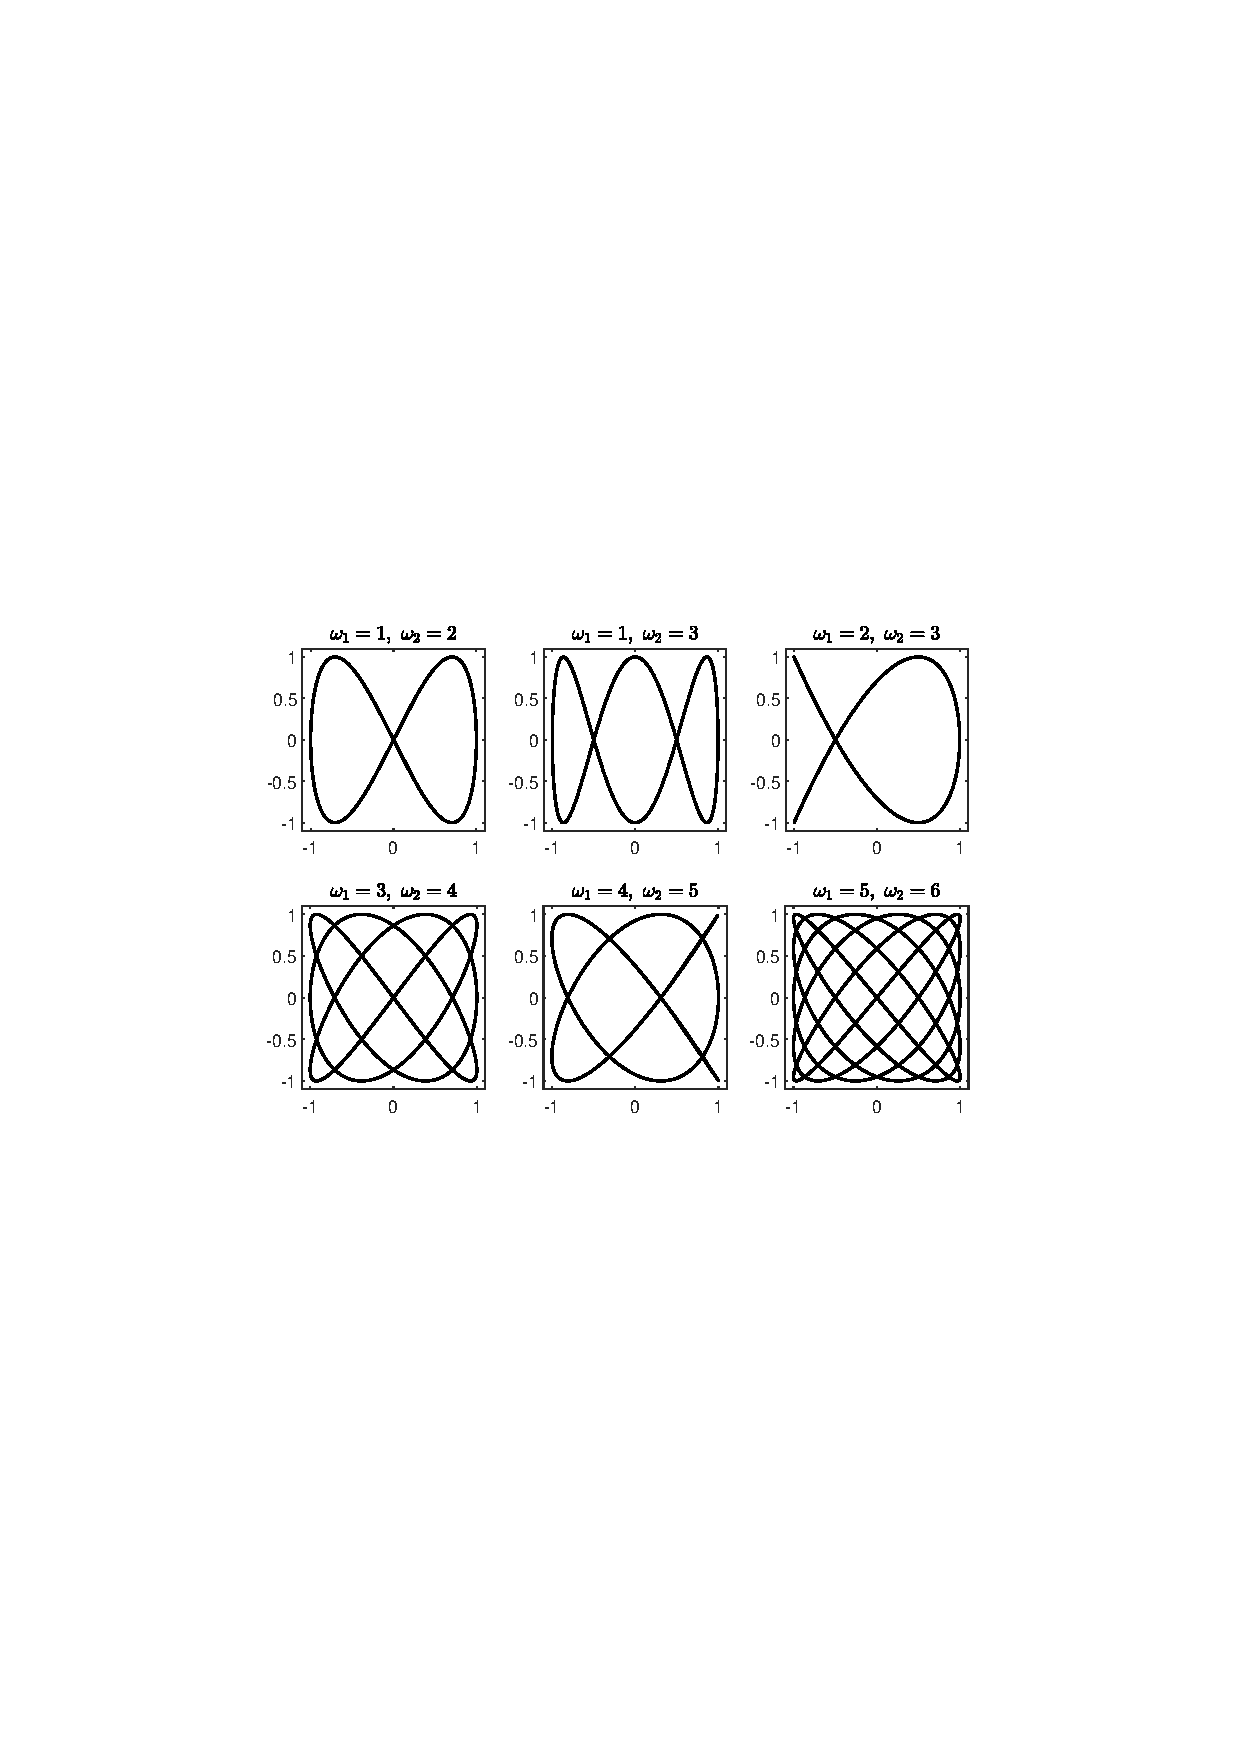
\includegraphics[width=0.95\linewidth]{李萨如图形}
\end{figure}

% ShangHai_2021GaoKao.m
\item 
(2021,上海高考)已知参数方程$ \begin{cases}
    & x=3t-4t^3 \\
    & y=2t\sqrt{1-t^2}
\end{cases} ,\ t\in [-1,1] $,下列选项的图中,符合该方程的是哪一个?
\begin{figure}[!htbp]
    \centering
    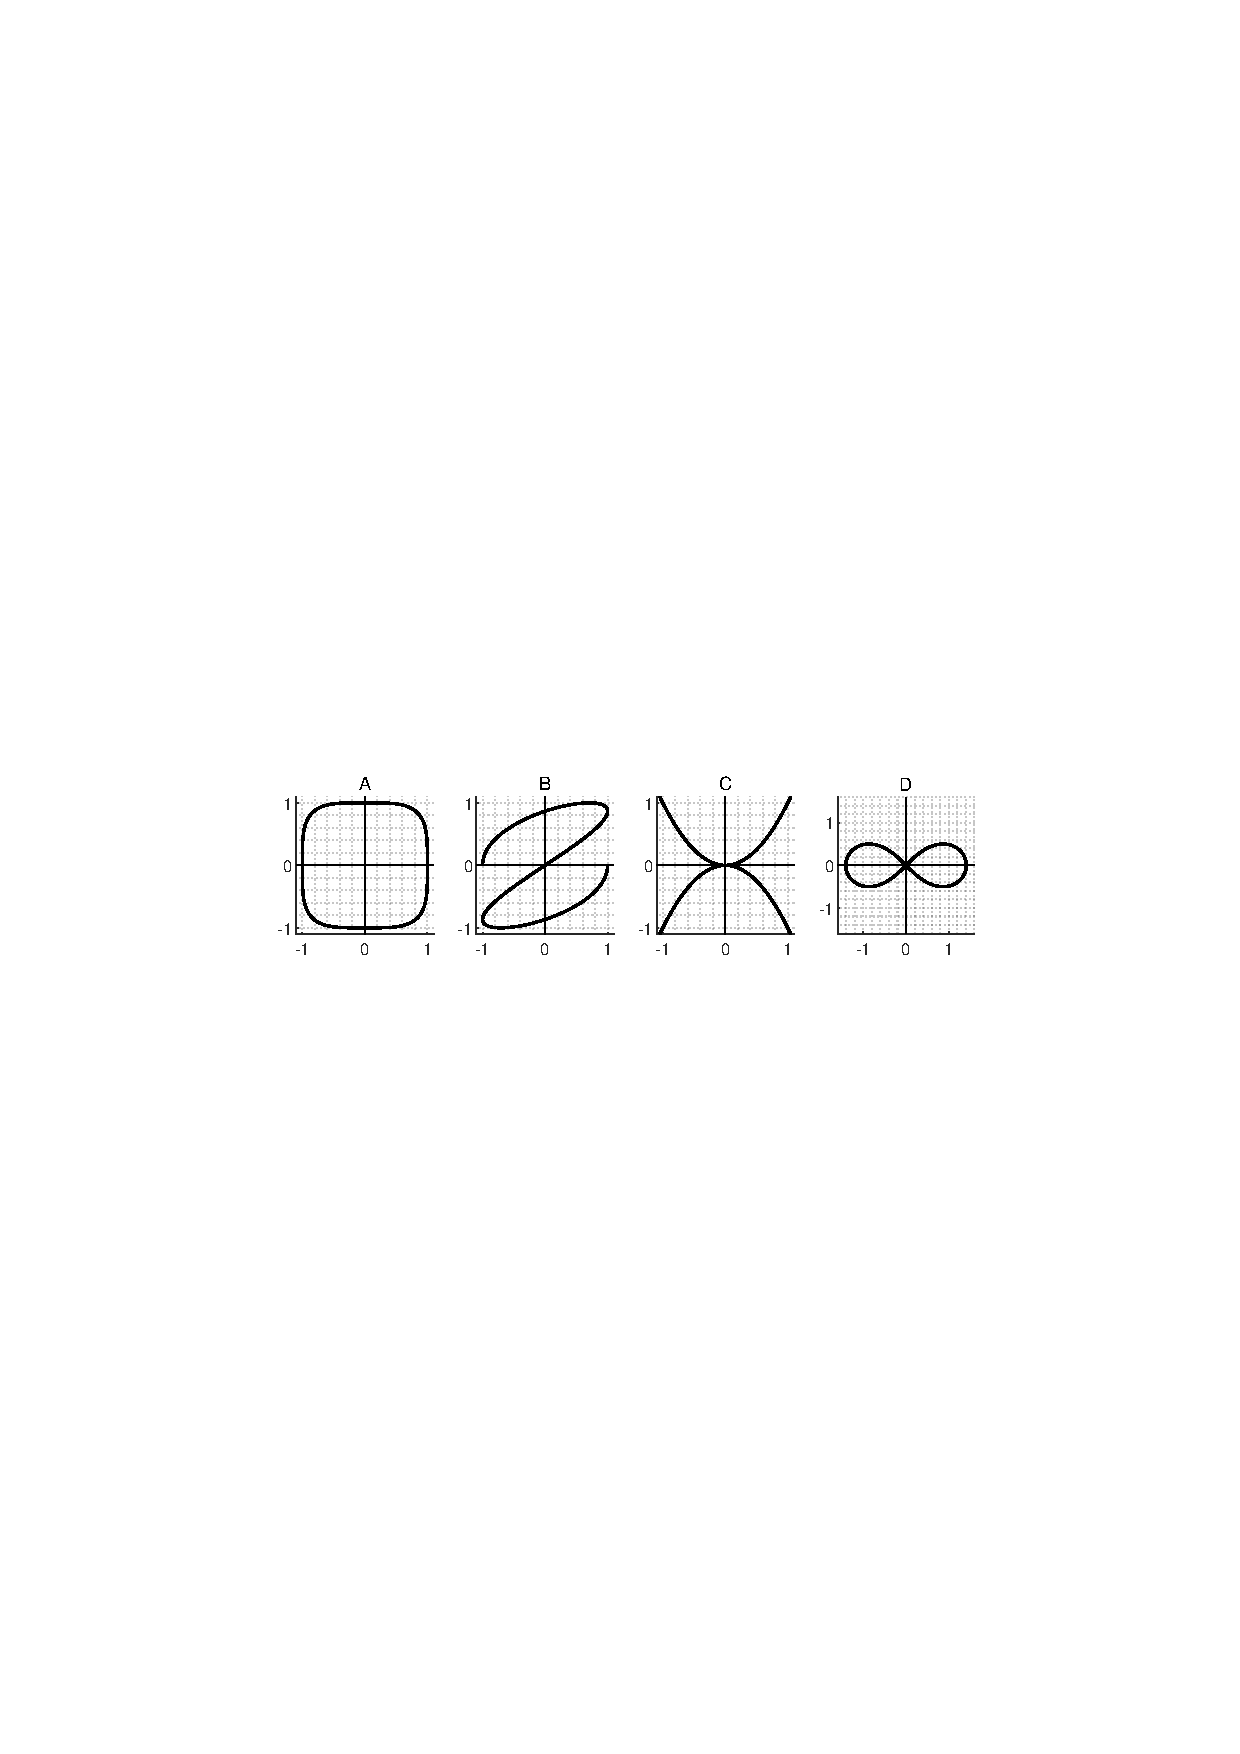
\includegraphics[width=1\linewidth]{2021上海高考参数曲线-李萨如}
\end{figure} \\
\textbf{解}\ 在参数方程中,如果把$ t $换成$ -t $,
那么$ (x,y) $会变成$ (-x,-y) $,
说明这条曲线是关于原点中心对称的,不过,4个选项的图形都是中心对称图形,
所以靠这一点无法排除。再考虑$ t $取特殊值,当$ t=0 $时,$ x=y=0 $,
所以可以排除A. 而当$ t=1 $时,$ x=-1,\ y=0 $,所以排除C、D,最终答案选B。

事实上,A对应的曲线大致是$ x^4+y^4=1 $. B对应的曲线是
\begin{align*}
    \begin{cases}
        & x=3t-4t^3=3\sin\theta-4\sin^3\theta=\sin3\theta \\
        & y=2t\sqrt{1-t^2}=2\sin\theta\cos\theta=\sin2\theta
    \end{cases},\ t=\sin\theta\in [-1,1],\ 
    \theta\in[-\dfrac{\pi}{2},\dfrac{\pi}{2}]
\end{align*}
这正是李萨如图形。如果让$ \theta $取值的区间长度达到$ 2\pi $,使曲线首尾相连变得完整,
那么它的形状如下
\begin{figure}[!htbp]
    \centering
    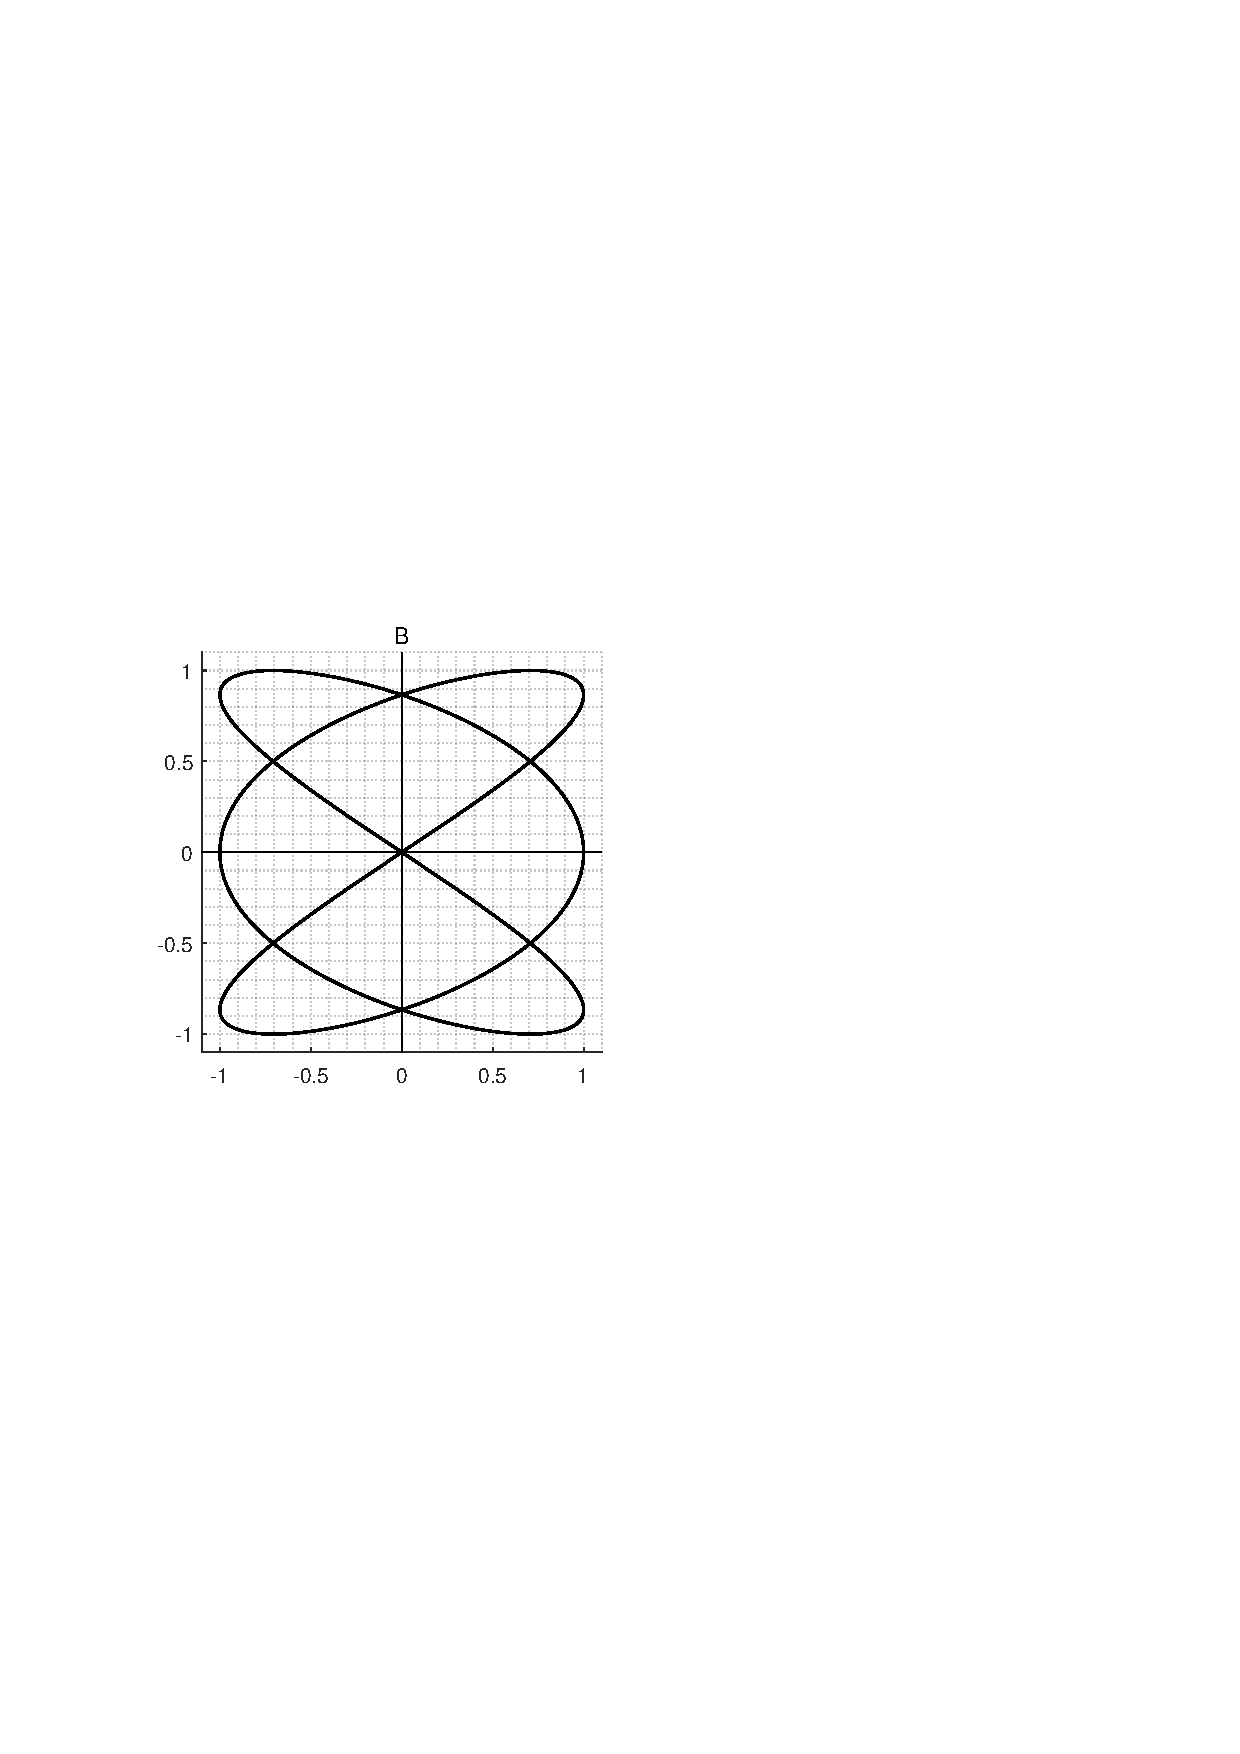
\includegraphics[width=0.3\linewidth]{2021上海高考参数曲线-李萨如B选项单独}
\end{figure} 

C对应的曲线是$ (y-x^2)(y+x^2)=0 $,D对应的曲线的极坐标方程是$ r^2=2\cos2\theta=
2(\cos^2\theta-\sin^2\theta) $,直角坐标方程是$ (x^2+y^2)^2=2(x^2-y^2) $,
这种曲线被称为双纽线。

\item (2021,新高考I卷)若$ \tan\theta=-2 $,求$ \dfrac{\sin\theta(1+\sin2\theta)}{
    \sin\theta+\cos\theta} $. \\
\textbf{方法一}\ 因为$ (\sin\theta+\cos\theta)^2=1+\sin2\theta $,所以
$ \dfrac{\sin\theta(1+\sin2\theta)}{\sin\theta+\cos\theta}=
\sin\theta(\sin\theta+\cos\theta) $. \\
假设$ \theta $为第二象限角,则$ \sin\theta=\dfrac{2\sqrt{5}}{5} $,
$ \cos\theta=-\dfrac{\sqrt{5}}{5} $,原式=$ \dfrac{2\sqrt{5}}{5}\Big(
\dfrac{2\sqrt{5}}{5}-\dfrac{\sqrt{5}}{5}\Big)=\dfrac{2}{5} $.\\
\textbf{方法二}\ 
\begin{gather*}
    \sin\theta(\sin\theta+\cos\theta)=\dfrac{\sin\theta(\sin\theta+\cos\theta)}
    {\sin^2\theta+\cos^2\theta}=\dfrac{\tan^2\theta+\tan\theta}{\tan^2\theta+1}
    =\dfrac{4-2}{4+1}=\dfrac{2}{5}
\end{gather*}
\textbf{方法三}\ 
\begin{align*}
    &\ \dfrac{\sin\theta(1+\sin2\theta)}{\sin\theta+\cos\theta} =
    \dfrac{\tan\theta(1+\sin2\theta)}{\tan\theta+1}=2(1+\sin2\theta) \\
    =&\ 2\left(1+\dfrac{2\sin\theta\cos\theta}{\sin^2\theta+
        \cos^2\theta}\right)=
    2\left(1+\dfrac{2\tan\theta}{\tan^2\theta+1}\right)=\dfrac{2}{5}
\end{align*}

\item \label{求tan2a例题}已知$ \sin\alpha+2\cos\alpha=\dfrac{\sqrt{10}}{2} $,
求$ \tan2\alpha $. \\
\textbf{方法一}\ 
\begin{gather*}
    (\sin\alpha+2\cos\alpha)^2=\left(\dfrac{\sqrt{10}}{2} \right)^2(\sin^2\alpha+\cos^2\alpha)  \\
    -\dfrac{3}{2}\sin^2\alpha+\dfrac{3}{2}\cos^2\alpha+4\sin\alpha \cos\alpha=0  
\end{gather*}
除以$ -\cos^2\alpha $以后可得$ 3\tan^2\alpha-8\tan\alpha-3=0 $,
解得$ \tan\alpha=3,-\dfrac{1}{3} $,两根之积为$ -1 $意味着两个$ \alpha $ 
角的终边相互垂直, $\tan2\alpha=\dfrac{2\tan \alpha}{1-\tan^2\alpha}=-\dfrac{3}{4} $. \\
\textbf{方法二}\ 二倍角公式:
\begin{gather*}
    -\dfrac{3}{2}\cdot\dfrac{1-\cos2\alpha}{2}+\dfrac{3}{2}\cdot\dfrac{1+\cos2\alpha}{2}
    +2\sin2\alpha=0  \\
    \dfrac{3}{2}\cos2\alpha+2\sin2\alpha=0 
\end{gather*}
\textbf{方法三}\ 解二次方程:$ 1-\cos^2\alpha=\sin^2\alpha=
\left(\dfrac{\sqrt{10}}{2}-2\cos\alpha \right)^2 $,
得到$ \cos\alpha=\dfrac{3}{\sqrt{10}} $,$ \sin\alpha=-\dfrac{1}{\sqrt{10}} $, $\tan\alpha=-\dfrac{1}{3} $,或者$ \cos\alpha=\dfrac{1}{\sqrt{10}}$, $\sin\alpha=\dfrac{3}{\sqrt{10}}$, $\tan\alpha=3 $,两种情况下都有$ \tan2\alpha=-\dfrac{3}{4} $. 

\item 对于已知$ \lambda_1\sin\alpha+\lambda_2\cos\alpha=\lambda_3 $的题目,
可设$ \lambda_1\cos\alpha-\lambda_2\sin\alpha=\lambda_4 $,
(注意不是$ \lambda_1\sin\alpha-\lambda_2\cos\alpha=\lambda_4 $),
将两式$ \begin{cases}
    \lambda_1\sin\alpha+\lambda_2\cos\alpha=\lambda_3 \\
    \lambda_1\cos\alpha-\lambda_2\sin\alpha=\lambda_4
\end{cases} $平方后相加可得:
\begin{gather*}
    \lambda_1^2+\lambda_2^2=\lambda_3^2+\lambda_4^2 
\end{gather*}
于是$ \lambda_4=\pm \sqrt{\lambda_1^2+\lambda_2^2-\lambda_3^2} $. 
在得到$ \lambda_4 $之后,可使用加减消元法解出$ \cos\alpha$ 和 $\sin\alpha $. \\
%利用 $ \dfrac{ \lambda_1\sin\alpha+\lambda_2\cos\alpha}{\lambda_1\cos\alpha-\lambda_2\sin\alpha} 
%    =\dfrac{\lambda_1\tan\alpha+\lambda_2}{\lambda_1-\lambda_2\tan\alpha} =\dfrac{\lambda_3}{\lambda_4}$,
%    可得到$ \tan\alpha $的值,也
% 这样更加方便,能避免解二次方程。

\item \label{分式三角求值域} 求$ k=\dfrac{4-\sin x}{3-\cos x} $的最值。\\
\textbf{方法一}\ 直接求导,令$ \left(\dfrac{4-\sin x}{3-\cos x}\right)'
=\dfrac{1-3\cos x-4\sin x}{(3-\cos x)^2}=0 $,把$ (\cos x,\sin x) $
看作是单位圆上的一点,那么$ 3\cos x+4\sin x=1 $正是单位圆的过点$ (3,4) $的切线,
($ k $可以看成是点$ (3,4) $与单位圆上一点的连线的斜率,在连线变成切线时,斜率有极值。)
解得$ \cos x=\dfrac{3\pm 8\sqrt{6}}{25},\sin x=\dfrac{4\mp 6\sqrt{6}}{25} $. 
于是最小值为$ \dfrac{6-\sqrt{6}}{4} $,最大值为$ \dfrac{6+\sqrt{6}}{4} $. \\
\textbf{方法二}\ $ k(3-\cos x)=4-\sin x,\ \underbrace{-k\cos x +\sin x=
    \sqrt{1+k^2}\sin(x+\varphi)}_{\text{辅助角公式}}=4-3k $,所以$ |4-3k|\leq\sqrt{1+k^2} $,
解得$ \dfrac{6-\sqrt{6}}{4}\leq k \leq \dfrac{6+\sqrt{6}}{4}  $. \\
$ |4-3k|\leq\sqrt{1+y^2} $可以变形为$ \dfrac{|4-3k|}{\sqrt{1+k^2}}
\leq 1 $,这个式子的含义就是圆心$ (0,0) $到直线$ y-4=k(x-3) $的距离小于等于半径1。\\
\textbf{方法三}\ 万能代换,令$ t=\tan\dfrac{x}{2}\in \textbf{R} $,则$ \sin x=
\dfrac{2\tan\frac{x}{2}}{1+\tan^2\frac{x}{2}}=\dfrac{2t}{1+t^2},\ \cos x=\dfrac{1-\tan^2\frac{x}{2}}{1+\tan^2\frac{x}{2}}=\dfrac{1-t^2}{1+t^2} $,
于是$ k=1+\dfrac{1-t}{2t^2+1} $,使用判别式法或者换元法(令$ 1-t=u $),可得
\begin{gather*}
    k\in \left[1+\dfrac{1}{-2\sqrt{6}-4}, 
    1+\dfrac{1}{2\sqrt{6}-4} \right]=\left[\dfrac{6-\sqrt{6}}{4},
    \dfrac{6+\sqrt{6}}{4}\right]
\end{gather*}
\textbf{注}:万能代换是计算含三角函数的积分的常用手段之一,比如求
$ \displaystyle{ \int\dfrac{(4-\sin x)}{3-\cos x}\d x } $
就可以使用万能代换。

\item 定义函数$ y=\dfrac{a+\sin x}{a+\cos x} $,其中$ |a|>1,x\in 
\textbf{R} $,$ y $的最大值记为$ M $,最小值记为$ m $,求$ M\cdot m $是多少。\\
\textbf{解}\ $ y=\dfrac{-a-\sin x}{-a-\cos x} $可看作点$ (-a,-a) $
与单位圆上一点的连线的斜率,在连线变成切线时,斜率有极值。本题中的两条切线是关于
直线$ y=x $对称的,所以$ M\cdot m=1 $. 还可以考虑极端情况,令$ |a|\to\infty $,
那么$ y\equiv 1,M=m=1 $,也能得到$ M\cdot m=1 $. 

\item 证明:$ \dfrac{\sin \mu\cos\mu-\sin\theta \cos\theta}
{\sin^2 \mu-\cos^2\theta}=\tan(\theta-\mu) $. \\
\textbf{证}\ 
\begin{align*}
    &\ \dfrac{\sin \mu\cos\mu-\sin\theta \cos\theta}
    {\sin^2 \mu-\cos^2\theta}
    = \dfrac{2\sin \mu\cos\mu-2\sin\theta \cos\theta}
    {2\sin^2 \mu-2\cos^2\theta}\\
    =&\ \dfrac{\sin2\mu-\sin2\theta}{(1-\cos2\mu)-(1+
        \cos2\theta)}
    = \dfrac{\sin2\theta-\sin2\mu}{\cos2\theta+
        \cos2\mu}\\
    =&\ \dfrac{2\cos(\theta+\mu)\sin(\theta-\mu)}{
        2\cos(\theta+\mu)\cos(\theta-\mu)}
    \quad \text{(使用和差化积公式)} \\
    =&\ \tan(\theta-\mu)
\end{align*}
以上运算过程会在使用“特征线”方法研究非线性超声速流动中遇到。

% XieJiBo_ShockWave.m
\item $ ^* $ 
已知$ M_1>1,\ 0<\beta<\dfrac{\pi}{2},\ \gamma>1,\ 0<\theta<\beta $,
又有
\begin{align*}
    \dfrac{\tan(\beta-\theta)}{\tan\beta}=\dfrac{2+(\gamma-1)M_1^2\sin^2\beta
    }{(\gamma+1)M_1^2\sin^2\beta}
\end{align*}
(I)求证:
\begin{align}\label{Q-B-M关系}
    \tan\theta=\dfrac{2(M_1^2\sin^2\beta-1)}{\tan\beta[M_1^2(\gamma+\cos2\beta)+2]}
\end{align} 
(II)\ $ M_{n1}=M_1\sin\beta,\ M_{n2}^2=\dfrac{1+\dfrac{\gamma-1}{2}M_{n1}^2}{
    \gamma M_{n1}^2-\dfrac{\gamma-1}{2}},\ M_2=\dfrac{M_{n2}}{\sin(\beta-
    \theta)} $,求证:
\begin{align}\label{斜激波比值等式}
    \dfrac{1+\dfrac{\gamma-1}{2}M_1^2}{1+\dfrac{\gamma-1}{2}M_2^2}=
    \dfrac{1+\dfrac{\gamma-1}{2}M_{n1}^2}{1+\dfrac{\gamma-1}{2}M_{n2}^2}
\end{align}
\textbf{证}\ (I)
\begin{align}\label{tanB_Q等式}
    \tan(\beta-\theta)=\dfrac{\tan\beta-\tan\theta}{1+\tan\beta\tan\theta}=
    \dfrac{[2+(\gamma-1)M_1^2\sin^2\beta]
        \tan\beta}{(\gamma+1)M_1^2\sin^2\beta}
\end{align}
\begin{align*}
    \tan\theta
    =&\ \dfrac{\tan\beta-\dfrac{[2+(\gamma-1)M_1^2\sin^2\beta]
            \tan\beta}{(\gamma+1)M_1^2\sin^2\beta}}
    {1+\dfrac{[2+(\gamma-1)M_1^2\sin^2\beta]
            \tan^2\beta}{(\gamma+1)M_1^2\sin^2\beta}} \\
    =&\ \dfrac{[(\gamma+1)M_1^2\sin^2\beta-2-(\gamma-1)M_1^2\sin^2\beta]\tan\beta}
    {(\gamma+1)M_1^2\sin^2\beta+2\tan^2\beta+(\gamma-1)M_1^2\sin^2\beta\tan^2\beta} \\
    =&\ \dfrac{2(M_1^2\sin^2\beta-1)\tan\beta}{\gamma M_1^2\sin^2\beta(1+\tan^2\beta)+
        M_1^2\sin^2\beta(1-\tan^2\beta)+2\tan^2\beta } \\
    =&\ \dfrac{2(M_1^2\sin^2\beta-1)}{\tan\beta[M_1^2(\gamma+\cos2\beta)+2]}
\end{align*}
(II) 先取一些具体的数字,让读者有直观的感受。令$ M_1=2,\ \beta=0.6,\ \gamma=1.4 $,
利用\eqref{tanB_Q等式}式,$ \tan(\beta-\theta)\approx 0.561071,\ 
\sin^2(\beta-\theta)=\dfrac{\tan^2(\beta-\theta)}{1+\tan^2(\beta-
    \theta)}\approx 0.239428 $,
$ M_{n1}=M_1\sin\beta\approx 1.129284 $,$ M_{n2}^2=\dfrac{
    1+\dfrac{\gamma-1}{2}M_{n1}^2}{\gamma M_{n1}^2
    -\dfrac{\gamma-1}{2}}\approx 0.791635 $,
$ M_2^2=\dfrac{M_{n2}^2}{\sin^2(\beta-\theta)}\approx 3.306351 $,那么
\begin{align*}
    \dfrac{1+\dfrac{\gamma-1}{2}M_1^2}{1+\dfrac{\gamma-1}{2}M_2^2}
    =1.083508\cdots=
    \dfrac{1+\dfrac{\gamma-1}{2}M_{n1}^2}{1+\dfrac{\gamma-1}{2}M_{n2}^2}
\end{align*}
下面给出严格证明,
将\eqref{斜激波比值等式}式左右交叉相乘,两边消去1,再约掉$ \dfrac{\gamma-1}{2} $,有
\begin{gather*}
    M_1^2+M_{n2}^2+\dfrac{\gamma-1}{2}M_1^2M_{n2}^2=
    M_2^2+M_{n1}^2+\dfrac{\gamma-1}{2}M_2^2M_{n1}^2   \\
    \left(1+\dfrac{\gamma-1}{2}M_1^2\right)M_{n2}^2-
    \left(1+\dfrac{\gamma-1}{2}M_{n1}^2\right)M_{2}^2=M_{n1}^2-M_1^2
    =-M_1^2\cos^2\beta \\
    \left[2+(\gamma-1)M_1^2-\dfrac{2+(\gamma-1) M_{n1}^2}{\sin^2(\beta-\theta)}
    \right]M_{n2}^2=-2M_1^2\cos^2\beta \\
    \left\{2+(\gamma-1)M_1^2-\dfrac{[2+(\gamma-1) M_{n1}^2][1+
        \tan^2(\beta-\theta)]}{\tan^2(\beta-\theta)}
    \right\}\dfrac{1+\dfrac{\gamma-1}{2}M_{n1}^2}{\gamma M_{n1}^2
        -\dfrac{\gamma-1}{2}}=-2M_1^2\cos^2\beta
\end{gather*}
将$ \tan(\beta-\theta) $用\eqref{tanB_Q等式}式右侧替换以后,只需验证下式成立:
\begin{gather*}
    \left[2+(\gamma-1)M_1^2\right]\left[2+(\gamma-1)M_{n1}^2\right]\sin^2\beta-
    \Big\{(\gamma+1)^2M_{n1}^4\cos^2\beta+\\ [2+(\gamma-1) M_{n1}^2]^2
    \sin^2\beta \Big\}=-4\left(\gamma M_{n1}^2-\dfrac{\gamma-1}{2}\right)
    M_1^2\sin^2\beta\cos^2\beta
\end{gather*}
(上式化简似乎没有特别的技巧,就是纯粹地去括号。) 证毕。 \\
\textbf{注}:(\ref{Q-B-M关系})式是空气动力学中用于研究激波的重要公式,
被称为$ \theta$-$\beta$-$M$关系
\footnote{ Anderson, John David. Fundamentals of Aerodynamics. McGraw-Hill(2005).Chapter 9, Oblique shock and expansion waves. \quad  或者参考 http://web.mit.edu/16.unified/www/SPRING/fluids/Spring2008/LectureNotes/f17.pdf}。$ M_1,\ M_2 $分别是斜激波前后的气流的马赫数。当$ M_1\to +\infty $时,$ \tan\theta=\dfrac{2\sin^2\beta}{\tan\beta(\gamma+\cos2\beta)}=\dfrac{\sin2\beta}{\gamma+\cos2\beta} $. 其中$ \gamma $是气体的绝热指数,与气体的成分、压强、温度有关,对于常温的空气,可以取$ \gamma=1.4 $. 利用\ref{分式三角求值域}的方法,可求出当$ \cos2\beta=-\dfrac{5}{7},\ \sin2\beta=\dfrac{\sqrt{24}}{7},\ \beta\approx 67.79^{\circ} $时,$ \dfrac{\sin2\beta}{\gamma+\cos2\beta} $取得最大值$ \dfrac{5\sqrt{6}}{12}=1.020620\cdots $,此时$ \theta_{\max}\approx\arctan1.02=45.5^{\circ} $\footnote{当$ \theta $超过$ \theta_{\max}=45.5^{\circ} $后,便无法在转角处产生附着的斜激波,而是产生脱体激波。在设计超声速飞行器(比如火箭、洲际弹道导弹、超声速战斗机等)的时候,不可避免地要研究激波。}. \\

%~\newpage
\end{enumerate}

\section{习题}
\begin{enumerate}[label={\textbf{\arabic*.}},leftmargin=
    \inteval{\myenumleftmargin}pt]
\item $ y=\cos(x^2) $与$ y=\cos(x^2+1) $,将其中一个函数的图像进行平移,
能否得到另外一个函数图像?

\item 用数学归纳法证明(\ref{余弦等差连加})和(\ref{正弦等差连加}).   

\item $ ^* $对(\ref{余弦等差连加})和(\ref{正弦等差连加})求导,计算
$ \sum\limits_{k=1}^{n}k\sin kx $和$ \sum\limits_{k=1}^{n}k\cos kx $. 
然后再利用数学归纳法证明。

\item 证明恒等式(\ref{三角恒等式2})$ \sim $ (\ref{三角恒等式-最后}).

\item 已知$ 2\sin\alpha+3\cos\alpha=\dfrac{\sqrt{26}}{2} $,求$ \tan2\alpha $.
(要求使用三种方法。)

\item 求三次函数$ f(x)=x^3+3x^2+6x-4 $的对称中心的坐标,
再用求根公式计算$ f(x)=0 $的实根,并写出韦达定理的三个式子。

\item 求复系数二次方程$ (2-4\i)x^2+2\i x+1=0 $的两个根。

\item 用尽可能多的方法求值域。\\
(1)\ $ y=\dfrac{3-\sin x}{2-\cos x} $ ;\quad 
(2)\ $ y=\dfrac{4-3\sin x}{3-2\cos x} $;\\
(3)\ $ y=\dfrac{4-3\sin x}{3-5\cos x} $;\quad
(4)\ $ y=\dfrac{4-6\sin x}{3-5\cos x} $.

\item 用二倍角公式和辅助角公式求$ y=2\sin^2 x+3\cos^2 x+4\sin x\cos x $
的最值和单调递增区间。感兴趣的还可尝试用万能代换求最值。

\item 求值: \\
(1) $ \cos\dfrac{\pi}{17}\cos\dfrac{2\pi}{17}\cos\dfrac{4\pi}{17}
\cos\dfrac{8\pi}{17} $. \\
(2) $ \cos\dfrac{\pi}{5}\cos\dfrac{2\pi}{5}\cos\dfrac{3\pi}{5}
\cos\dfrac{4\pi}{5} $. \\
(3) $ \sin\dfrac{\pi}{5}\sin\dfrac{2\pi}{5}\sin\dfrac{3\pi}{5}
\sin\dfrac{4\pi}{5} $. \\
(4) $ \cos\dfrac{\pi}{7}+\cos\dfrac{3\pi}{7}+\cos\dfrac{5\pi}{7} $. \\
(5) $ \cos\dfrac{\pi}{9}+\cos\dfrac{3\pi}{9}+\cos\dfrac{5\pi}{9}+\cos\dfrac{7\pi}{9} $. 

\item 求$ 15^{\circ},18^{\circ},22.5^{\circ},36^{\circ} $
的正弦、余弦、正切的根式表达式,如果结果包含二重根式,请尝试去掉外层根式。


\item 求证:在锐角$ \Delta ABC $中,\\
(I) $ \sin A +\sin B +\sin C > \dfrac{4}{3} (\cos A +\cos B +\cos C) $. \\
(II) $ \tan^2 A+\tan^2 B +\tan^2 C \geq 9 $.


\item 求证:在$ \Delta ABC $中,\\ $ \sin (nA) +\sin (nB) +\sin (nC)=
\begin{cases}
    -& 4\sin(\dfrac{nA}{2})\sin(\dfrac{nB}{2})\sin(\dfrac{nC}{2}),\quad 
    n=4k \\
    & 4\cos(\dfrac{nA}{2})\cos(\dfrac{nB}{2})\cos(\dfrac{nC}{2}),\quad 
    n=4k+1 \\
    & 4\sin(\dfrac{nA}{2})\sin(\dfrac{nB}{2})\sin(\dfrac{nC}{2}),\quad 
    n=4k+2 \\
    -& 4\cos(\dfrac{nA}{2})\cos(\dfrac{nB}{2})\cos(\dfrac{nC}{2}),\quad 
    n=4k+3
\end{cases} $

\item $ \i $是虚数单位,求$ 1+3\i+5\i^2+7\i^3+\cdots +4039\i^{2019} $的值。


\item 找出以下列数值为根的整系数方程(要求方程的次数尽量低)。\\
(1)\ $ \sqrt{2}+\sqrt{5} $ \quad (2) $ 1+\sqrt{3}+\sqrt{5} $ \quad (3) 
$ \sqrt{3}+\sqrt[3]{3} $ 

\item$^*$  用只含$ \cos x $或$ \cos x $的幂的式子表达
$ \cos 7x,\cos 8x,\cos 9x $. 

\item$ ^* $ 用软件绘制$ \sin(x^2)+\sin(y^2)=1 $的图像。\\
$\diamond$ GeoGebra、Desmos、MathStudio:直接输入
\verb|sin(x^2)+sin(y^2)=1|即可。\\
$\diamond$ MATLAB语法:
\begin{lstlisting}
syms x y
fimplicit(sin(x.^2) + sin(y.^2) == 1,'meshdensity',2000)
axis([-10 10 -10 10])    
\end{lstlisting} 
$\diamond$ Maple语法:
\begin{lstlisting}
with(plots, implicitplot)
implicitplot(sin(x^2) + sin(y^2) = 1, x = -10 .. 10, 
y = -10 .. 10, gridrefine = 9, resolution = 1000)    
\end{lstlisting} 
$\diamond$ Mathematica语法:
\begin{lstlisting}
ContourPlot[Sin[x^2]+Sin[y^2]==1, {x, -10, 10}, {y, -10, 10}]    
\end{lstlisting} 

感兴趣的读者可进一步探索$ \sin(x^{\alpha})+\sin(y^{\alpha})=1,\ 
\sin\left(x^{2}+y^{2}\right)=\cos\left(x\cdot y\right) $的图像,
以及把$ \sin $换成$ \cos,\tan $后的图像。

\end{enumerate}

\section{习题答案}
\begin{enumerate}[label={\textbf{\arabic*.}},leftmargin=
    \inteval{\myenumleftmargin}pt]

% cos_x2_PingYi.m
\item 不能。两者图像如下:
\begin{figure}[h]
    \centering
    \includegraphics[width=0.9\linewidth]{cos(x2)与cos(x2+1)}
\end{figure} \\
两者都是偶函数,所以只需考虑$ x>0 $的部分。可以这样思考:
两个函数从左到右第$ k $个极大值点的横坐标之差不是常数,即
\begin{gather*}
    \sqrt{2k\pi}-\sqrt{2k\pi-1}=\dfrac{1}{\sqrt{2k\pi}+\sqrt{2k\pi-1}}\to 0
\end{gather*}

\item 略

\item \begin{align*}
    &\sum_{k=1}^{n}k\sin kx=\dfrac{-n\cos(n+\dfrac{1}{2})x\sin\dfrac{x}{2}+
        \dfrac{1}{2}\sin nx}{2\sin^2 \dfrac{x}{2}} \\
    &\sum_{k=1}^{n}k\cos kx=\dfrac{n\sin(n+\dfrac{1}{2})x\sin\dfrac{x}{2}+
        \dfrac{1}{2}\cos nx - \dfrac{1}{2}}{2\sin^2 \dfrac{x}{2}} 
\end{align*}
数学归纳法过程略。

\item 略

\item 模仿\ref{求tan2a例题}即可,
$ \tan\alpha=-\dfrac{1}{5},5,\ \tan2\alpha=-\dfrac{5}{12} $.  

\item 对称中心$ (-1,-8) $. 作变换$ x=t-1 $,则原方程变为
$ t^3+3t-8=0 $,$ p=3,\ q=-8 $,
$ \Delta=\dfrac{q^2}{4}+\dfrac{p^3}{27}=17 $,原方程实根为:
\begin{align*}
    x =\sqrt[3]{4+\sqrt{17}}+\sqrt[3]{4-\sqrt{17}}-1=0.512745\cdots
\end{align*}
韦达定理:$ x_1+x_2+x_3=-3,\ x_1x_2+x_1x_3+x_2x_3=6,\ x_1x_2x_3=-4 $. 

\item $ -\dfrac{1}{10}+\dfrac{3}{10}\i,\ 
\dfrac{1}{2}-\dfrac{1}{2}\i $. 

\item
(1)$ |2y-3|\leq \sqrt{y^2+1},\ \dfrac{6-2\sqrt{3}}{3}\leq y\leq \dfrac{6+2\sqrt{3}}{3} $. \\
(2)$ |3y-4|\leq \sqrt{4y^2+9},\ \dfrac{12-\sqrt{109}}{5}\leq y\leq \dfrac{12+\sqrt{109}}{5} $. \\
(3)$ |3y-4|\leq \sqrt{25y^2+9},\ y\leq -\dfrac{7}{4},\ y\geq\dfrac{1}{4} $. \\
(4) \textbf{R}.

\item
$ y=\dfrac{1}{2}\cos 2x+2\sin2x+\dfrac{5}{2}=
\dfrac{\sqrt{17}}{2}\sin(2x+\varphi)+\dfrac{5}{2} $,
其中,$ \cos\varphi=\dfrac{4}{\sqrt{17}} $, $ \sin\varphi=\dfrac{1}{\sqrt{17}} $. 
最值为$ \dfrac{5\pm \sqrt{17}}{2} $,单调递增区间为$ [k\pi-\dfrac{\pi}{4}-\dfrac{\varphi}{2},k\pi+\dfrac{\pi}{4}-\dfrac{\varphi}{2}],\ k\in \textbf{Z} $. \\
万能代换后,$ y=\dfrac{3t^4-8t^3+2t^2+8t+3}{(t^2+1)^2}=3-\dfrac{4(2t^3+t^2-2t)}
{(t^2+1)^2} $,令$ f(t)=\dfrac{2t^3+t^2-2t}{(t^2+1)^2} $,则$ f'(t)=
\dfrac{-2(t^4+t^3-6t^2-t+1)}{(t^2+1)^3} $,分子中的四次多项式$ t^4+t^3-6t^2-t+1 $在有理数域内无法因式分解,所以万能代换会遇到困难。

\item
(1)根据(\ref{余弦等比连乘})式,
$ \dfrac{\sin\dfrac{16\pi}{17}}{16\sin\dfrac{\pi}{17}}=\dfrac{1}{16} $. \\
(2)根据(\ref{余弦等差连乘})式,$ \dfrac{1}{16} $. \\
(3)根据(\ref{正弦等差连乘})式,$ \dfrac{5}{16} $. \\
(4)根据(\ref{余弦等差连加})式,$ \cos\dfrac{\pi}{7}+\cos\dfrac{3\pi}{7}+\cos\dfrac{5\pi}{7}=
-\left(\cos\dfrac{6\pi}{7}+\cos\dfrac{4\pi}{7}+\cos\dfrac{2\pi}{7}\right)= \\
-\dfrac{\sin(3+\dfrac{1}{2})\dfrac{2\pi}{7}-\sin\dfrac{\pi}{7}}{2\sin\dfrac{\pi}{7}}=\dfrac{1}{2} $. \\
(5) $ \dfrac{1}{2} $. 

\item 如下表:
\begin{table}[h]
    \centering
    \begin{tabular}{l|l|l}
        $ \sin(15^{\circ})=\dfrac{\sqrt{6}-\sqrt{2}}{4} $ & 
        $ \cos(15^{\circ})=\dfrac{\sqrt{6}+\sqrt{2}}{4} $ & 
        $ \tan(15^{\circ})=2-\sqrt{3}$ \\ [9pt]
        $ \sin(22.5^{\circ})=\dfrac{\sqrt{2-\sqrt{2}}}{2} $ & 
        $\cos(22.5^{\circ})=\dfrac{\sqrt{2+\sqrt{2}}}{2}$ & 
        $ \tan(22.5^{\circ})=\sqrt{2}-1 $ \\ 
        [9pt]		
        $ \sin(18^{\circ})=\dfrac{\sqrt{5}-1}{4} $ & 
        $\cos(18^{\circ})=\dfrac{\sqrt{10+2\sqrt{5}}}{4} $ &
        $ \tan(18^{\circ})=\dfrac{\left(5-\sqrt{5}\right)
            \sqrt{10-2\sqrt{5}}}{20} $ \\ [9pt]	
        $ \sin(36^{\circ})=\dfrac{\sqrt{10-2\sqrt{5}}}{4} $ & $\cos(36^{\circ})=\dfrac{\sqrt{5}+1}{4} $ &
        $ \tan(36^{\circ})=\dfrac{\left(\sqrt{5}-1\right)
            \sqrt{10-2\sqrt{5}}}{4} $ \\ [9pt]
    \end{tabular} 
\end{table}

\item (1) 当$ x\in\Big(0,\dfrac{\pi}{2}\Big) $时,
$ \sin x>\dfrac{2}{\pi}x $,所以
\begin{gather*}
    \sin A +\sin B +\sin C>\dfrac{2}{\pi}(A+B+C)=2
\end{gather*}
根据(\ref{三个余弦和不等式-小于})式,$ \cos A +\cos B +\cos C\leq \dfrac{3}{2} $,
所以,
\begin{gather*}
    \sin A +\sin B +\sin C>2 \geq \dfrac{4}{3} (\cos A +\cos B +\cos C)
\end{gather*}
事实上有更强的不等式:
\begin{gather*}
    \sin A +\sin B +\sin C>\Big(1+\dfrac{\sqrt{2}}{2}\Big)(\cos A +\cos B +\cos C)
\end{gather*}
只有当三角形为等腰直角三角形时,上面的不等号才能变成等号;对于钝角三角形,上式不成立。\\
(2)
\begin{align*}
    &\ \tan^2 A+\tan^2 B +\tan^2 C \\
    \geq &\ \dfrac{1}{3}(\tan A+\tan B +\tan C)^2\q (\text{柯西不等式}) \\
    \geq &\ \dfrac{1}{3}\Big(3\tan\dfrac{A+B+C}{3}\Big)^2\q 
    (\text{正切函数的凹凸性}) \\
    = &\ 9
\end{align*}
$ A=B=C=\dfrac{\pi}{3} $时,等号成立。

\item 略

\item $ (-4-4\i)\times \dfrac{2020}{4}=-2020-2020\i $. 

\item (1)$ x^4-14x^2+9 $\quad (2) $ x^4-4x^3-10x^2+28x-11 $ \\
(3) $ x^6-9x^4-6x^3+27x^2-54x-18 $

\item
\begin{align*}
    & 64\cos^7x-112\cos^5x+56\cos^3x-7\cos x \\
    & 128\cos^8x-256\cos^6x+160\cos^4x-32\cos^2x+1 \\
    & 256\cos^9x-576\cos^7x+432\cos^5x-120\cos^3x+9\cos x
\end{align*}

\end{enumerate}

\myfootnote{\CopyrightStatementChap}
% {\footnotesize (可在以下空白区域自行增补知识点。)}  
\cleardoublepage

